\section{Physics Requirements for {\tt CLAS12} Tracking}

The {\tt CLAS} detector in Hall B is being upgraded to take advantage of 
the increase of the CEBAF beam energy from 6 to 12~GeV, thus the new name,  
{\tt CLAS12}.  There are several broad areas of physics enquiry that drive 
these changes: spectroscopic studies of excited baryons, investigations of 
the influence of nuclear matter on propagating quarks, studies of polarized 
and unpolarized quark distributions, and a comprehensive measurement of 
generalized parton distributions (GPDs).  Many of the reactions of interest 
are electroproduction of exclusive and semi-inclusive final states.  The 
cross sections for these processes are small, necessitating high-luminosity 
experiments.  A variety of simulated experiments rely on luminosities of 
10$^{35}$~cm$^{-2}$s$^{-1}$ to achieve the desired statistical accuracy in 
runs of a few months duration.  The new kinematic range to be explored is 
characterized not only by smaller cross sections, but also by more outgoing 
particles per event, with those particles being emitted with higher values 
of momentum and at smaller laboratory angles.  These basic physics criteria 
drive the design. 

The deep exclusive reactions, in which an electron scattering at moderate to 
high values of $Q^2$ results in a meson-baryon final state, provide the most 
stringent requirements for the {\tt CLAS12} tracking system.  A final state 
of a few high-momentum, forward-going particles (the electron as well as one 
or more mesons), combined with a moderate-momentum baryon emitted at large 
angles, is the typical event type that determines the specifications of the 
tracking system.

The higher momentum and more forward angles of most hadrons leads us to 
split the design into a ``forward'' detector, which covers lab angles between 
5$^\circ$ and 40$^\circ$, and a ``central'' detector for hadrons with angles 
greater than 35$^\circ$.  The higher luminosity goal necessitates the use of 
a solenoidal magnet to shield the detector from M{\o}ller electrons.  To 
reduce interactions between this solenoidal field and the main {\tt CLAS12} 
toroidal field, and to facilitate construction and installation of new 
detector elements, the torus has been re-designed.  It is more compact than 
the present {\tt CLAS} torus, while providing equivalent bending power.  This 
smaller torus design provides several advantages in the overall detector 
design: it decouples the design of the central solenoid and detector from 
that of the torus and forward tracking system, and it makes detector 
installation and removal easier.  

In broad strokes, the detector must provide tracking for laboratory angles as 
small as 5$^\circ$ and as large as 125$^\circ$ in order to cover as much of 
the hadronic center-of-mass region as possible.  We require very good momentum 
and angular resolution for the scattered electron in order to determine the 
virtual photon flux factor, $\Gamma_v$, to an accuracy of a few percent.
Because the average particle momenta will be higher, the resolution of the 
tracking system must be better than the current {\tt CLAS} values; the goal 
for the fractional momentum resolution is 0.5\% to 1\% at a track momentum 
of 5~GeV.  Angular resolutions of about 1~mrad are required for the electron 
in order to know the virtual photon flux factor, and hence, the cross section, 
to a few percent. Finally, good vertex resolution will allow detection of 
secondary decay vertices and serve as a good marker for strangeness production.

Because only about 20\% of the total charged particle momenta is carried by 
tracks in the central region, the fractional momentum resolution requirement
for the central tracking system at a momentum of 1~GeV is 5\% in order to 
match the absolute momentum resolution of the forward tracking system.  This 
momentum resolution of about 50~MeV is necessary in order to positively 
identify a missing pion in these exclusive reactions.  Similarly, to keep our 
knowledge of the individual vector components of the momentum at the 25~MeV 
level, the central trackers angular resolution should be of the order of 
1.5$^\circ$.  Our present design has an expected performance about a factor 
of two better than these simple limits.  

A tracking system capable of achieving these standards was described in the 
PCDR~\cite{pcdr} and quantitatively parameterized in a ``fast'' Monte Carlo 
program~\cite{fastmc}.  A number of {\tt CLAS} collaborators used the model 
of the detector as described in FASTMC in proposals presented at JLab 
PAC30 and PAC32~\cite{PAC30,PAC32}.

%%%%%%%%%%%%%%%%%%%%%%%%%%%%%%%%%%%%%%%%%%%%%%%%%%%%%%%%%%%%%%%%%%%%%%%
\begin{figure}[ht]
\centering
\includegraphics[width=0.60\textwidth]{clas12_system}
\caption{\small{A three-dimensional view of the proposed {\tt CLAS12} 
detector highlighting the various subsystems.}}
\label{clas12}
\end{figure}
%%%%%%%%%%%%%%%%%%%%%%%%%%%%%%%%%%%%%%%%%%%%%%%%%%%%%%%%%%%%%%%%%%%%%%%

\section{Tracking System Design}

As noted above, the {\tt CLAS12} detector is divided into a forward and a 
central detector.  Fig~\ref{clas12} shows a perspective view of the 
{\tt CLAS12} detector.  A solenoid magnet surrounds the target,  followed 
by a M{\o}ller absorber on the beam-line and a high-threshold {\v C}erenkov 
counter for electron identification.  Besides curling background M{\o}ller 
electrons into the absorber, the solenoid provides a nearly constant magnetic 
field that allows charged particle momentum determination by a set of 
``central tracking chambers'' consisting of 8 layers of silicon strip sensors.
This central tracking region covers polar angles from 35$^\circ$ to 
125$^\circ$.  Just downstream of the cylindrical central tracker are the 
``forward vertex chambers'': 6 layers of silicon strip chambers.  Downstream 
of the high-threshold {\v C}erenkov counter is the torus magnet that supports 
three ``regions'' of ``forward drift chambers'', designated as Regions~1, 2, 
and 3.  Surrounding and downstream of the torus/drift chamber assembly are 
the forward time-of-flight counters, a low-threshold {\v C}erenkov counter 
for hadron identification, and two sets of electromagnetic shower counters.  
This document describes each of the elements of the {\tt CLAS12} tracking 
system, the central tracker, the forward vertex tracker, and the forward 
drift chambers.

We have designed the tracking detectors with these external constraints: a 
solenoid of 5~T central field value and a radius available for tracking 
detectors of 25~cm, a new torus with a different aspect ratio but with the 
same number of amp-turns as the present {\tt CLAS} torus, an expected
background rate consistent with a luminosity of 10$^{35}$~cm$^{-2}$s$^{-1}$, 
and a separation between the ``forward'' and ``central'' regions defined to 
be at about 40$^\circ$; specifically the forward tracking chambers are 
designed to cover scattering angles between 5$^\circ$ and 40$^\circ$ and the 
central tracker will cover 35$^\circ$ to 125$^\circ$.  Although the torus 
cryostat will limit the azimuthal coverage to about 50\% at 5$^\circ$, our 
goal is that the inactive portion of the drift chambers not further intrude 
into the active volume; i.e. the dead areas of the drift chambers (endplates, 
electronics, etc.) will be located in the ``shadow'' of the coil as viewed 
from the target.  For Region~2, this is not possible; but we shall try to 
minimize this dead area.  To summarize, we are designing the {\tt CLAS12} 
tracking system with the requirements shown in Table~\ref{tracker-specs}.

%%%%%%%%%%%%%%%%%%%%%%%%%%%%%%%%%%%%%%%%%%%%%%%%%%%%%%%%%%%%%%%%%%%%%%%%%
\begin{table}[htbp]
\begin{center}
\begin{tabular} {||l|c|c||} \hline \hline
                    & {\bf Fwd. Tracker }    & {\bf Central Tracker} \\ \hline
Angular coverage    & 5$^\circ$ - 40$^\circ$ & 35$^\circ$ - 125$^\circ$  \\ \hline
Momentum resolution & $dp/p < 1$$\%$         & $dp/p < 5$$\%$            \\ \hline
$\theta$ resolution & 1~mrad                 & 1~mrad                    \\ \hline
$\theta$ resolution & 1~mrad                 & 5 - 10~mrad               \\ \hline
$\phi$ resolution   & 1~mrad/$\sin \theta$   & 5~mrad/$\sin \theta$      \\ \hline
Luminosity          & 10$^{35}$~cm$^{-2}$s$^{-1}$ & 10$^{35}$~cm$^{-2}$s$^{-1}$ \\ \hline \hline
\end{tabular}
\caption{\small{General specifications for {\tt CLAS12} tracking.}}
\label{tracker-specs}
\end{center}
\end{table}
%%%%%%%%%%%%%%%%%%%%%%%%%%%%%%%%%%%%%%%%%%%%%%%%%%%%%%%%%%%%%%%%%%%%%%%%%

\subsection{Forward Tracking Design}

The higher beam energies available to {\tt CLAS12} mean that tracks will go 
more forward and have higher momenta than for the present {\tt CLAS} 
experiments.  We thus require better resolution from the forward drift 
chambers.  Our design should give better spatial resolution than the present 
{\tt CLAS} chambers for several reasons: the use of thicker (30-$\mu$m 
diameter) sense wires will result in a more linear drift velocity, all cells 
in a superlayer will be identical, easing the calibration, and the simpler 
mechanical structure should make these chambers easier to survey.  The other 
feature of higher energy and associated smaller cross sections, requires the 
use of higher intensity beams.  The resultant higher backgrounds represent 
the primary motivation for the central solenoidal magnet and M{\o}ller 
absorber.  The higher background can also be mitigated by cells that cover a 
smaller angular range and have a smaller active time window.

Forward tracks (angles between 5$^\circ$ and 40$^\circ$) will be 
momentum-analyzed by passing through the magnetic field of the torus.  The 
magnet provides an integral $Bdl$ of almost 3 T-m at 10$^\circ$, falling
to about 1 T-m at 30$^\circ$ (see Fig.~\ref{bdl}).

%%%%%%%%%%%%%%%%%%%%%%%%%%%%%%%%%%%%%%%%%%%%%%%%%%%%%%%%%%%%%%%%%%%%%%%%%%%
\begin{figure}[htbp]
\vspace{6.8cm}
\special{psfile=btoro1.ps hscale=55 vscale=40 hoffset=90 voffset=-10}
\caption{\small{The integral of the $B$ field times path length along rays 
from the target at various angles.}}
\label{bdl}
\end{figure}
%%%%%%%%%%%%%%%%%%%%%%%%%%%%%%%%%%%%%%%%%%%%%%%%%%%%%%%%%%%%%%%%%%%%%%%%%%%

Such forward tracks will first pass through six layers of the forward silicon 
vertex tracker (FST); a silicon strip tracker with a strip pitch of 
150~$\mu$m arranged with alternating $V$-$W$ stereo layers with a stereo angle 
of $\pm$12$^\circ$, located about 27~cm from the target.  These tracks will 
then traverse the high-threshold {\v C}erenkov counter (HTCC) before 
entering the Region~1 drift chamber at a distance of 2.1~m from the target.  
The track continues through the magnetic field region and its trajectory is 
measured in two more drift chambers, denoted Regions~2 and 3, respectively.  
The Region~2 and 3 chambers are located at 3.3 and 4.5~m from the target,
respectively.  The FST should localize hits with an estimated accuracy of 
about 50~$\mu$m perpendicular to the strip direction, while the three regions 
of drift chambers are expected to have spatial resolutions of about
250~$\mu$m per layer.  The expected momentum resolution from such an assembly 
is a function of angle, ranging from about 0.3\% at 5$^\circ$ to about 1.0\% 
at 30$^\circ$, and nearly constant as a function of momentum.  The angular 
resolution falls rapidly with increasing momentum, but should be better than 
2~mrad at a momentum of 1~GeV.

\subsection{Central Tracking Design}

The momentum and angular resolution goals for the central tracker are set by 
the requirement that we be able to positively identify a single missing pion; 
roughly a 50~MeV momentum resolution is needed, i.e. a fractional momentum 
resolution of 5\% or better at a track momentum of 1~GeV.  Our design consists 
of 8 layers of silicon strips with alternating plus and minus stereo angle 
strips.  Each detector plane is formed as a polygonal shell with the silicon
strips running along the $z$-direction.  Each single-sided layer is comprised 
of 300-$\mu$m thick silicon.  This detector has good intrinsic resolution in 
the $r$-$\phi$ coordinate due to the small strip pitch (150~$\mu$m readout and 
75~$\mu$m implant pitch). It relies on a small stereo angle to determine the 
$r$-$z$ position of tracks.  

A solenoidal magnet contains the target, the silicon vertex tracker, the 
central time-of-flight system (CTOF), and the M{\o}ller absorber.  Charged 
particles with emission angles greater than 35$^\circ$ follow helical paths 
through the 8 layers of the BST, which are arranged into four $V$-$W$ modules 
with ``$V$'' and ``$W$'' referring to strip orientations.  The time resolution 
of the CTOF ($\sim$60~ps) will enable particle identification of the charged 
tracks, as well as allowing for a very efficient rejection of out-of-time 
accidentals.

\section{Silicon Vertex Tracker for {\tt CLAS12}}

\subsection{Overview}

The Silicon Vertex Tracker (SVT), anticipated to have $\sim$65,000 channels, 
will consist of a forward silicon tracker (FST) and a barrel silicon tracker 
(BST).  The $\theta$-coverage  of the forward part is from 5$^\circ$ to 
35$^\circ$ and that of the barrel part is from 35$^\circ$ to 125$^\circ$.  
Conceptual design studies started in 2004~\cite{CN2004-42}.  For both the 
forward and barrel parts, the $\phi$ coverage is nearly $2\pi$.  The SVT will 
be centered inside the 1800-mm long solenoid, that has an outer and inner 
diameter of 2040~mm and 780~mm, respectively
.
%%%%%%%%%%%%%%%%%%%%%%%%%%%%%%%%%%%%%%%%%%%%%%%%%%%%%%%%%%%%%%%%%%%%%%%
\begin{figure}[htbp]
\centering
\includegraphics[width=0.65\textwidth]{solenoid}
\caption{\small{Side view of the solenoid magnet (units in inches -- with mm 
in parentheses).}}
\label{fig:solenoid}
\end{figure}
%%%%%%%%%%%%%%%%%%%%%%%%%%%%%%%%%%%%%%%%%%%%%%%%%%%%%%%%%%%%%%%%%%%%%%%

\subsection{Configuration}

Several configurations of the BST and the FST were studied~\cite{CN2006-21} 
with the aim to optimize the layout with respect to operability, performance 
and cost.  The BST is designed to have four regions and the FST is designed 
to have three regions.  The BST and FST form two independent detectors (see
Fig.~\ref{side-svt-layout}), providing operational flexibility in that either 
or both detectors could be used in a given experiment. There are only three 
FST regions because the FST will be used in conjunction with the three drift 
chambers in the forward region.   

%%%%%%%%%%%%%%%%%%%%%%%%%%%%%%%%%%%%%%%%%%%%%%%%%%%%%%%%%%%%%%%%%%%%%%%
\begin{figure}[htbp]
\centering
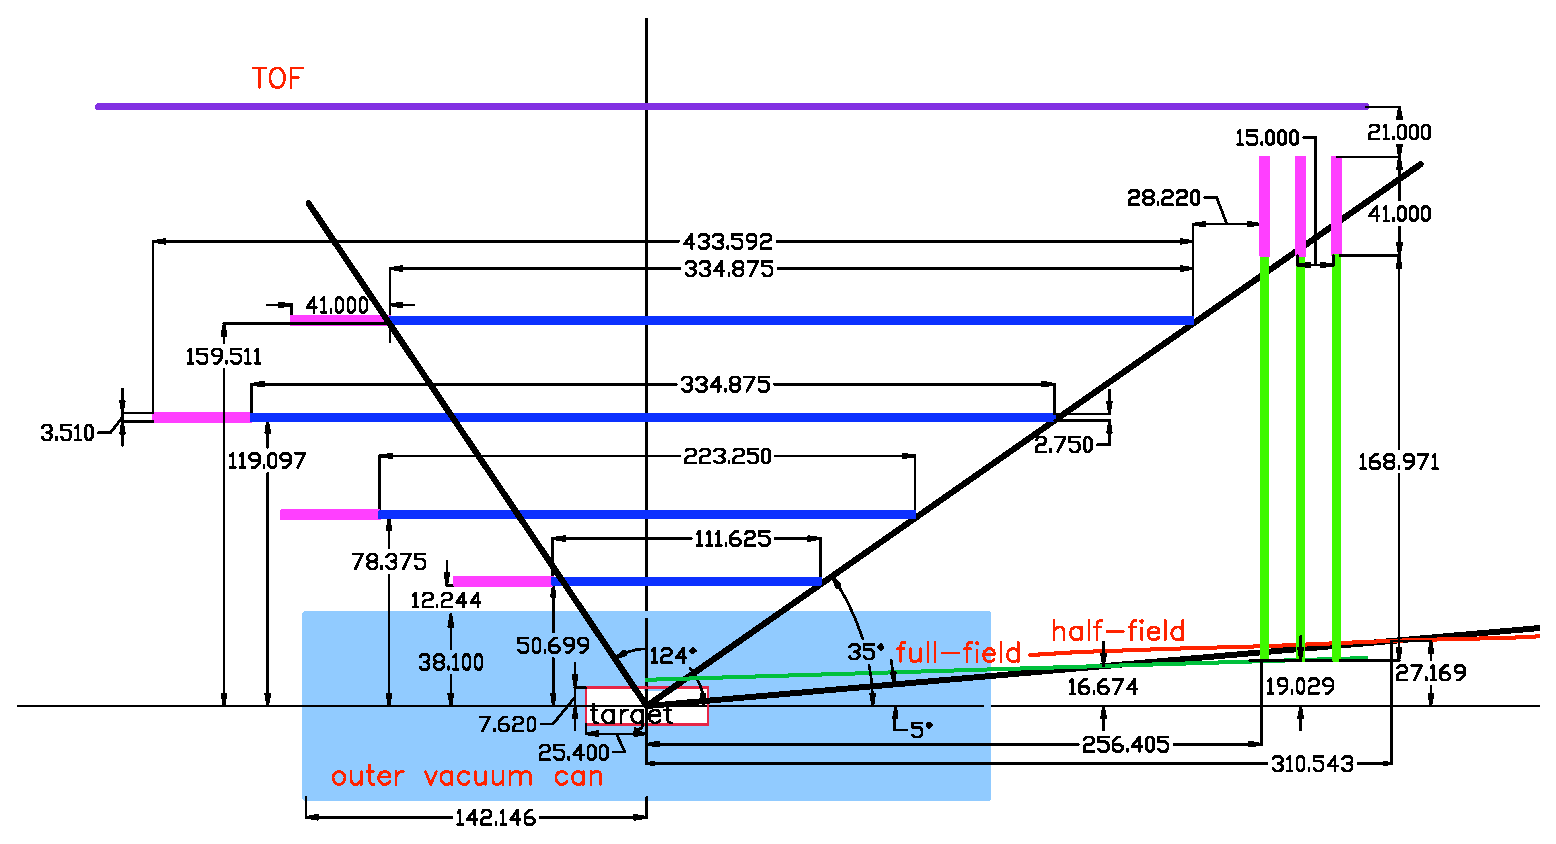
\includegraphics[width=0.9\textwidth]{side-view2a}
\caption{\small{Side view of the SVT showing the layout of the barrel and 
forward regions (all dimensions in mm).}}
\label{side-svt-layout}
\end{figure}
%%%%%%%%%%%%%%%%%%%%%%%%%%%%%%%%%%%%%%%%%%%%%%%%%%%%%%%%%%%%%%%%%%%%%%%

%%%%%%%%%%%%%%%%%%%%%%%%%%%%%%%%%%%%%%%%%%%%%%%%%%%%%%%%%%%%%%%%%%%%%%%
\begin{figure}[htbp]
\centering
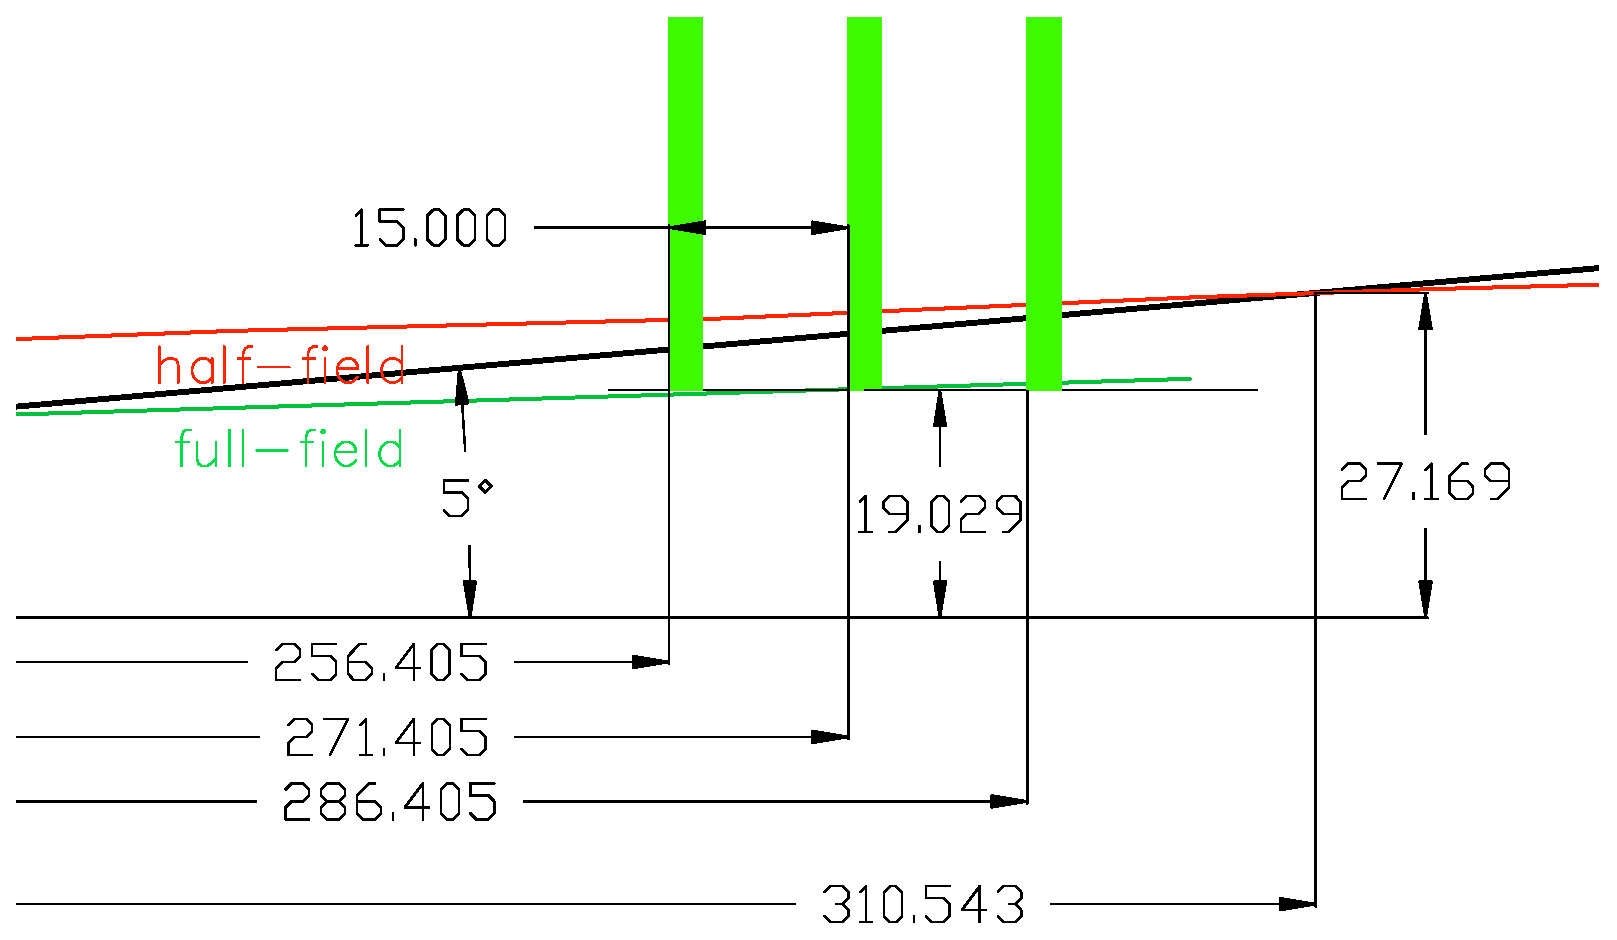
\includegraphics[width=0.9\textwidth]{cone_beam}
\caption{\small{Close up view of the three forward SVT regions near the beam 
line and the M{\o}ller absorber.}}
\label{cone_beam}
\end{figure}
%%%%%%%%%%%%%%%%%%%%%%%%%%%%%%%%%%%%%%%%%%%%%%%%%%%%%%%%%%%%%%%%%%%%%%%

\subsection{Rate Estimates}

Event and background rates were estimated using a GEANT simulation
\cite{CN2004-13,CN2006-20}.  These studies indicate that the maximum rate, 
including electromagnetic background for a full-field setting of the solenoid 
(5~T) is $\sim$40~MHz in the FST and $\sim$60~MHz in the BST.  In 
Fig.~\ref{side-svt-layout}, the green and red curve (full and half-field 
settings of the solenoid) along the beam axis is the M{\o}ller electron 
envelope, on the surface of which the rate is $\sim$1~MHz. The rate drops 
rapidly with increasing scattering angle~\cite{CN2006-20}.

To keep M{\o}ller electron rates on the FST sensors less than 1~MHz, the first 
region of the FST is placed at $z$=256.405~mm (see Figs.~\ref{side-svt-layout} 
and \ref{cone_beam}), past the intersection of the M{\o}ller electron envelope 
for the full-field setting with the keep-out zone, defined to be a cone with 
a half opening angle of 5$^\circ$.  The second and third regions of the FST 
are at $z$=271.405~mm and $z$=286.405~mm, respectively.

\subsection{Forward Silicon Tracker (FST)}

The trapezoidal sensors of the FST are designed to be identical.  Such a 
design requires that the regions be parallel to the beam axis, rather than 
ride the 5$^\circ$ keep-out cone.  In $\phi$, each FST region consists of 15 
sectors as shown in Fig.~\ref{fig:front-cone}.  

%%%%%%%%%%%%%%%%%%%%%%%%%%%%%%%%%%%%%%%%%%%%%%%%%%%%%%%%%%%%%%%%%%%%%%%
\begin{figure}[htbp]
\centering
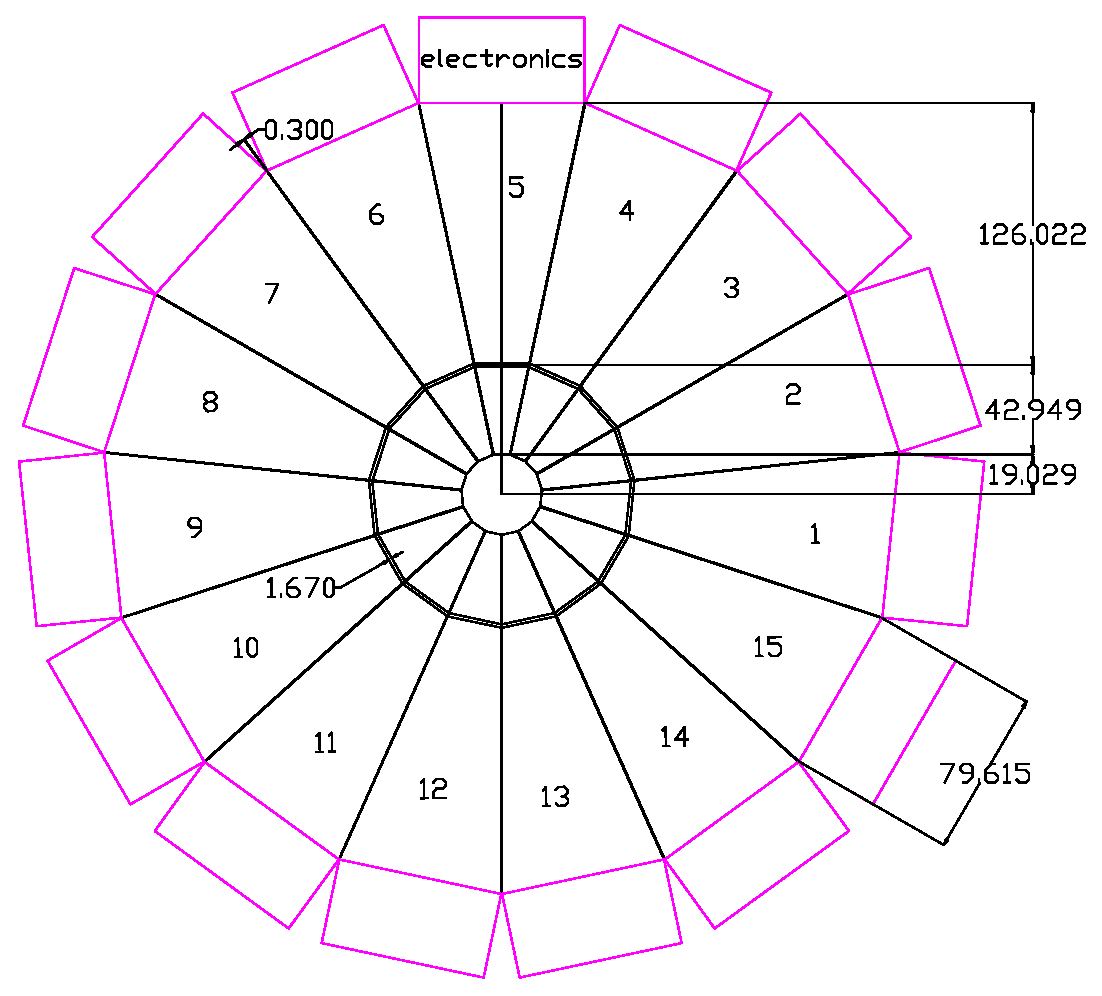
\includegraphics[width=0.5\textwidth]{front-cone}
\caption{\small{Front view of the first region of the FST showing the
layout and positioning of the trapezoidal sensors.}}
\label{fig:front-cone}
\end{figure}
%%%%%%%%%%%%%%%%%%%%%%%%%%%%%%%%%%%%%%%%%%%%%%%%%%%%%%%%%%%%%%%%%%%%%%%

In the critical region around the beam axis at $r\sim$19~mm, because the 
sensors are trapezoidal, the $V$ and the $W$ layers of a region each have 
$\sim$40 strips per sector, distributed over 2$\pi$, a total of $\sim$600 
strips per layer.  The rate near the beam axis has to be handled by these 
600 strips.  Though 600 strips per layer around the beam axis appears to be 
a small number, the readout electronics associated with these strips will 
on average have a rate-load of $\sim$10~kHz that can be handled by the 
readout electronics.

%%%%%%%%%%%%%%%%%%%%%%%%%%%%%%%%%%%%%%%%%%%%%%%%%%%%%%%%%%%%%%%%%%%%%%%
\begin{figure}[htbp]
\centering
\includegraphics[width=0.8\textwidth]{rear-barrel}
\caption{\small{Rear view of the barrel section of the SVT showing the
sensor partitioning in each region.}}
\label{fig:rear-barrel}
\end{figure}
%%%%%%%%%%%%%%%%%%%%%%%%%%%%%%%%%%%%%%%%%%%%%%%%%%%%%%%%%%%%%%%%%%%%%%%

\subsection{Barrel Silicon Tracker (BST)}

The four BST regions have $\sim$240~mm of radial space available for tracking.
Having four regions instead of the minimum three needed for track 
reconstruction provides a redundant tracking region that mitigates the risk of 
tracking inefficiencies due to layer problems such as malfunctioning strips, 
electronics, or noise.  Further, tracking simulations indicate that with four 
regions instead of three, the probability of reconstructing fake tracks for a 
given number of correlated background hits per region (that are randomly 
distributed over the four BST regions) is reduced by a factor of three.  Our 
simulations indicate that four regions should be able to handle about forty 
background hits in the time window.  The first BST region has a diameter of 
$\sim$101~mm.  The second, third, and fourth BST regions have diameters of 
$\sim$157~mm, $\sim$239~mm, and $\sim$320~mm, respectively.  The radial 
distance, $\Delta r$, between region four and region one of the BST has been 
chosen to maximize momentum resolution, which has an inverse square dependence 
on $\Delta r$.  In $\phi$, the BST regions, from the innermost to the 
outermost, are partitioned in 8, 12, 18, and 24 sectors, as shown in 
Fig.~\ref{fig:rear-barrel}.  Studies indicate that track loss due to the 
cracks between adjacent sectors in the BST is less than 5\% for a half-field 
setting of the solenoid, as long as the cracks are no wider than 2~mm.

\subsection{Dicing Layout}

The dicing layout for a trapezoidal sensor from a 6-in diameter wafer is 
shown in Fig.~\ref{fig:trap-dicing}.  The dicing process demands a 
keep-out zone of 0.25~in around the edge of the wafer.

%%%%%%%%%%%%%%%%%%%%%%%%%%%%%%%%%%%%%%%%%%%%%%%%%%%%%%%%%%%%%%%%%%%%%%%
\begin{figure}[htbp]
\centering
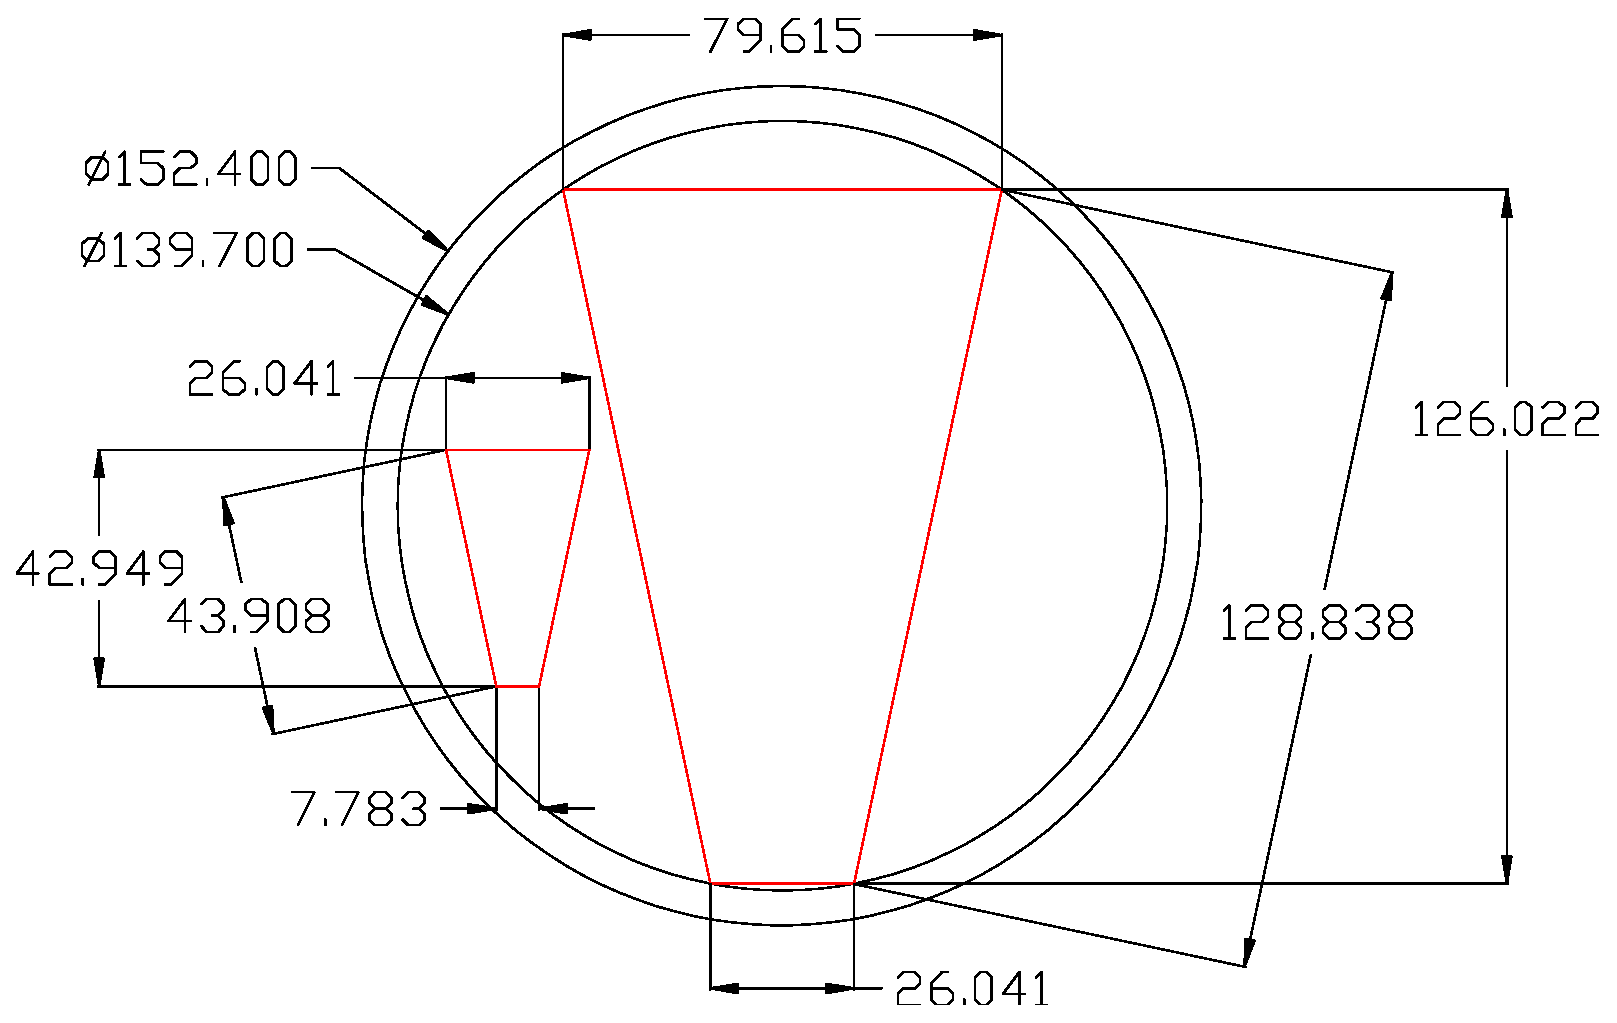
\includegraphics[width=0.6\textwidth]{trap-dicing}
\caption{\small{Trapezoidal sensor dicing from a standard 6-in wafer. All 
units in mm.}}
\label{fig:trap-dicing}
\end{figure}
%%%%%%%%%%%%%%%%%%%%%%%%%%%%%%%%%%%%%%%%%%%%%%%%%%%%%%%%%%%%%%%%%%%%%%%


The BST dicing layout of a 6-in wafer, as shown in 
Fig.~\ref{fig:barrel-dicing}, is such that it provides the longest sensors 
possible.  Such a layout reduces the number of sensors needed for the BST 
modules.  Further, cost is reduced by maximizing the yield of sensors from a 
single wafer -- minimizing the total number of wafers required for the BST.  
All BST regions use sensors with a cut size of 111.62~mm $\times$ 42.00~mm 
$\times$ 0.300~mm.

%%%%%%%%%%%%%%%%%%%%%%%%%%%%%%%%%%%%%%%%%%%%%%%%%%%%%%%%%%%%%%%%%%%%%%%
\begin{figure}[htbp]
\centering
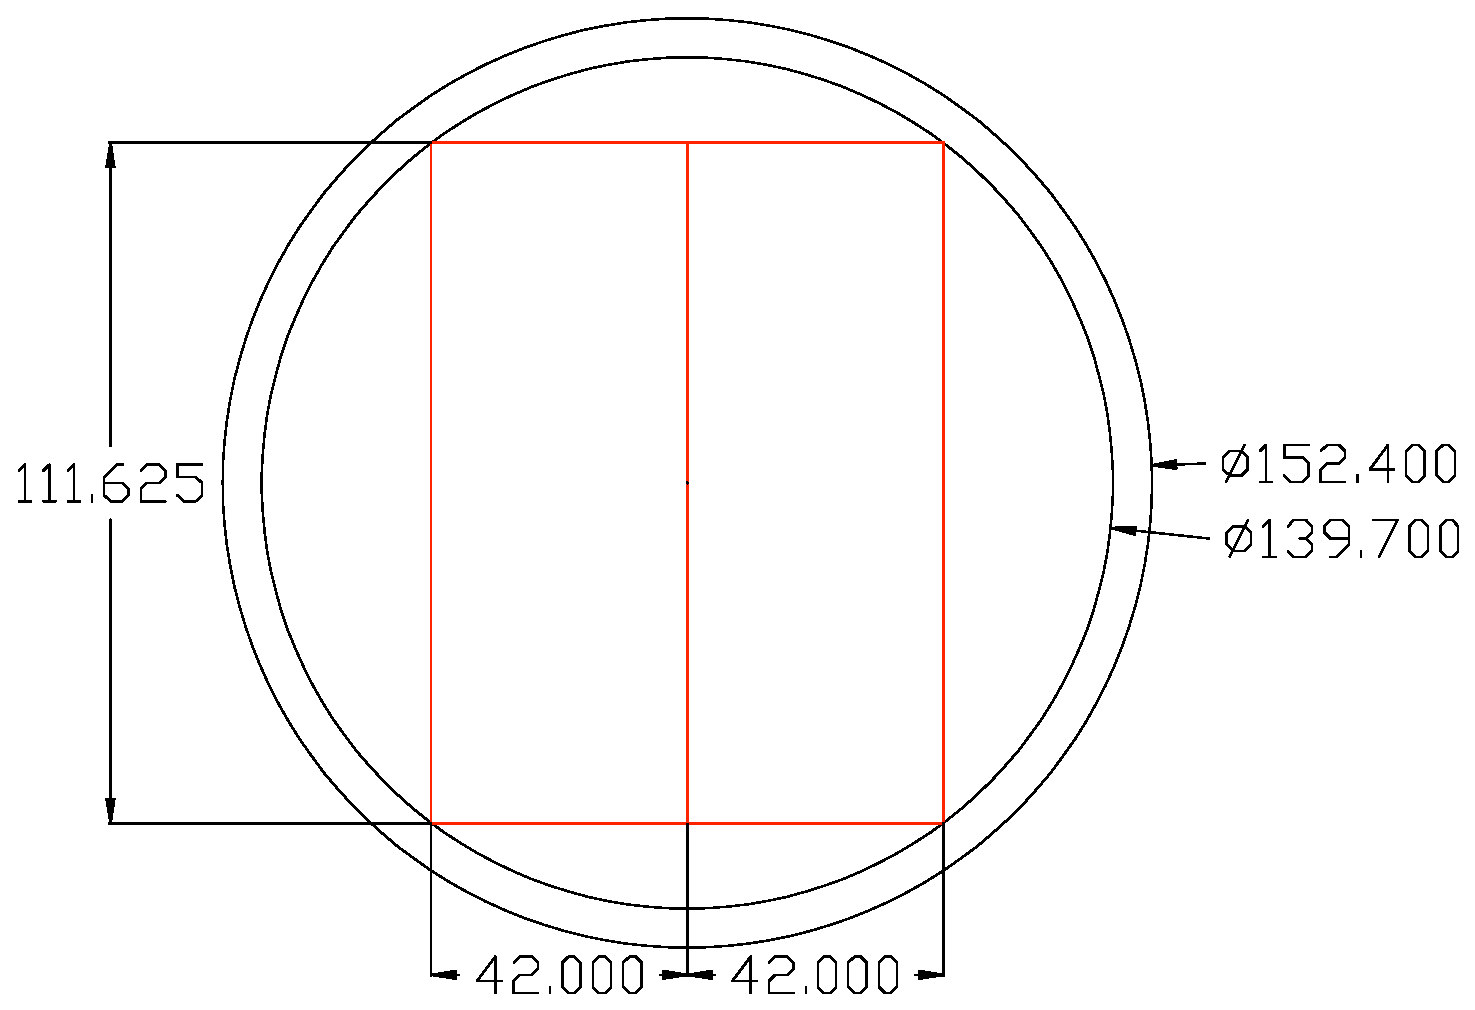
\includegraphics[width=0.6\textwidth]{barrel-dicing}
\caption{\small{Barrel sensor dicing from a standard 6-in wafer. All units 
in mm.}}
\label{fig:barrel-dicing}
\end{figure}
%%%%%%%%%%%%%%%%%%%%%%%%%%%%%%%%%%%%%%%%%%%%%%%%%%%%%%%%%%%%%%%%%%%%%%%

\subsection{Module and Strip Layout}

Fig.~\ref{fig:sensor-detail} shows the cross sectional view of the sensor.  
The lengths of the readout strips of the SVT vary from 0.5~cm to 33~cm.  The 
strip width is $\sim$8~$\mu$m and the implant depth $\sim$1.2~$\mu$m.

%%%%%%%%%%%%%%%%%%%%%%%%%%%%%%%%%%%%%%%%%%%%%%%%%%%%%%%%%%%%%%%%%%%%%%%
\begin{figure}[htbp]
\centering
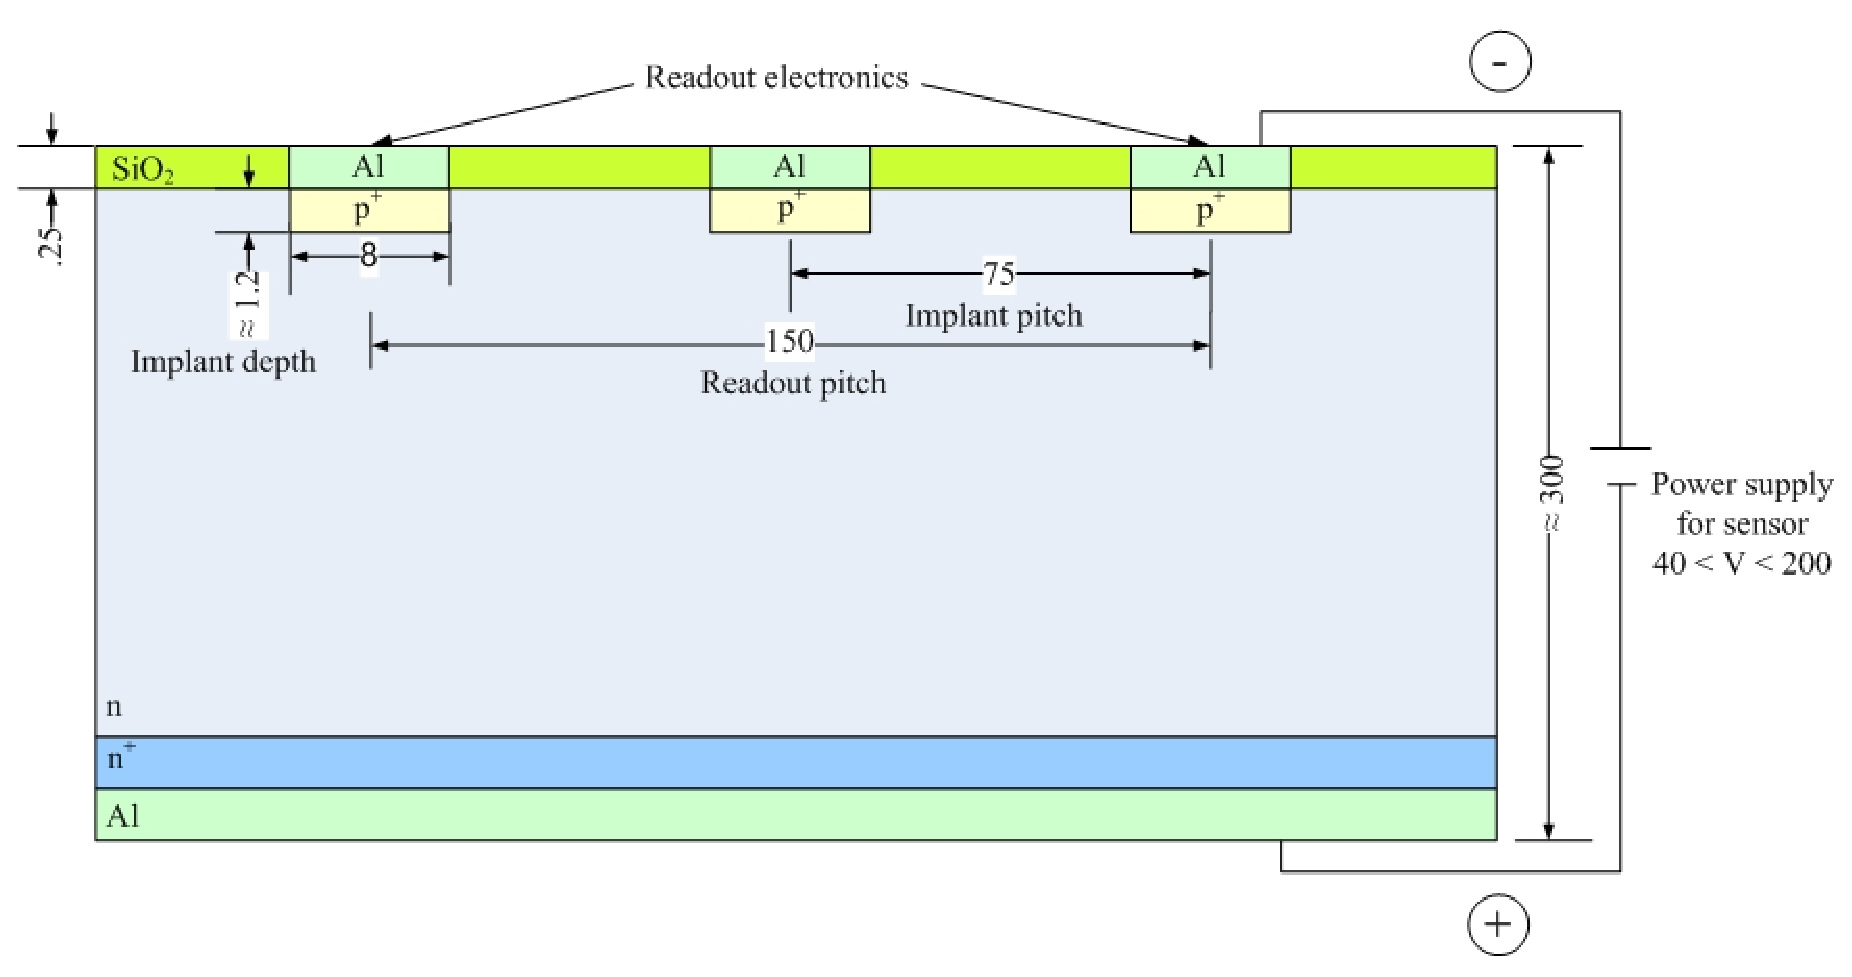
\includegraphics[width=0.7\textwidth]{sensor-detail}
\caption{\small{Cross sectional view of a sensor showing the different
layers and the spacing of the strips (all units in $\mu$m).}}
\label{fig:sensor-detail}
\end{figure}
%%%%%%%%%%%%%%%%%%%%%%%%%%%%%%%%%%%%%%%%%%%%%%%%%%%%%%%%%%%%%%%%%%%%%%%

A completed module in the BST has 256 readout channels per layer -- 512 
channels in all per module.  The modules of the FST have 512 channels per 
layer -- 1024 channels total per module.  Each FST sector consists of a 
module -- a single trapezoidal unit as shown in Fig.~\ref{fig:trap-dicing} 
that consists of a $V$ and a $W$ silicon layer that sandwich a 2-mm-thick 
Rohacell~71 carbon fiber composite.   

To reduce costs, the $V$ and $W$ layers for the modules of the different 
BST regions are made of one or more fundamental rectangular sensors.  If 
more than one sensor is needed for a module, the sensors are wire-bonded 
together.  Modules of the BST Regions 1, 2, 3, and 4 have 1, 2, 3, and 3 
sensors, respectively (see Fig.~\ref{side-svt-layout}).  Fig.~\ref{svt_views}
shows 3D renderings of how the complete SVT system is expected to look.  

%%%%%%%%%%%%%%%%%%%%%%%%%%%%%%%%%%%%%%%%%%%%%%%%%%%%%%%%%%%%%%%%%%%%%%%
\begin{figure}[htbp]
\vspace{6.7cm}
\special{psfile=overall-rear.eps hscale=33 vscale=33 hoffset=0 
voffset=0}
\special{psfile=overall-side.eps hscale=33 vscale=33 hoffset=245 
voffset=0}
\caption{\small{Overall conceptual renderings for the SVT showing a rear
view (left) and a side view (right).}}
\label{svt_views}
\end{figure}
%%%%%%%%%%%%%%%%%%%%%%%%%%%%%%%%%%%%%%%%%%%%%%%%%%%%%%%%%%%%%%%%%%%%%%%

Table~\ref{matprop} gives the radiation length of the materials used for 
the sensor structure.  Because of the large variety of commercial graphite 
fibers available for GFRP (glass fiber reinforced polymer) composites, they 
have an added bonus of being easily obtainable at an acceptable cost.  The 
preferred structural materials are GFRP and Rohacell.  The total anticipated 
radiation length for the BST is $\sim$3.5\% and for the FST $\sim$2.7\%. 

%%%%%%%%%%%%%%%%%%%%%%%%%%%%%%%%%%%%%%%%%%%%%%%%%%%%%%%%%%%%%%%%%%%%%%%
\begin{table}[htbp]
\begin{center}
\begin{tabular}{|c|c|c|c|} \hline
Material & Radiation Length (mm) & Thickness (mm) & Radiation Length [\%X0] 
\\ \hline
Silicon    &   93.7 & 0.300 & 0.320 \\ \hline
Epoxy      &  443.7 & 0.025 & 0.007 \\ \hline
GFRP       &  250.0 & 0.250 & 0.100 \\ \hline
Rohacell71 & 5450.0 & 2.000 & 0.040 \\ \hline
GFRP       &  250.0 & 0.250 & 0.100 \\ \hline
Epoxy      &  443.7 & 0.025 & 0.007 \\ \hline
Silicon    &   93.7 & 0.300 & 0.320 \\ \hline 
\end{tabular}
\end{center}
\caption{\small{Material thickness with radiation lengths for the different
layers that make up the sensors of the BST and FST.}}
\label{matprop}
\end{table}
%%%%%%%%%%%%%%%%%%%%%%%%%%%%%%%%%%%%%%%%%%%%%%%%%%%%%%%%%%%%%%%%%%%%%%%

The readout pitch for the strips, which is twice the implant pitch, is 
determined by the minimization, as far as affordable, of spatial resolution.  
Based on this criterion, the strips are designed to have an implant pitch of 
0.075~mm and a readout pitch of 0.150~mm.  The expected spatial resolution 
for this pitch spacing is about 0.050~mm and the occupancy in a layer of an 
FST region, for half-field operation of the solenoid, is less than $\sim$1.5\%.
The $V$ and $W$ layer strips for the FST sensors run parallel to the edges of 
the trapezoid (see Fig.~\ref{fig:trap-strip}), with the strips intersecting at 
an angle of 12$^\circ$.

For the BST, the 42-mm width of the sensor accommodates 256 input 
channels, at a readout strip pitch of 0.150~mm, to the two SVX4 ASICs, and 
the required keep-out zones around the sensor (see Fig.~\ref{barrel_strip}).  
The $V$ and $W$ strips are designed such that strip 1 is at an 
angle of 0$^\circ$ with respect to the length axis of the rectangular BST 
sensors and strip 256 is at an angle of 3$^\circ$.  This was done to minimize
sensor dead area.  Details are shown in Fig.~\ref{barrel_strip}.  

%%%%%%%%%%%%%%%%%%%%%%%%%%%%%%%%%%%%%%%%%%%%%%%%%%%%%%%%%%%%%%%%%%%%%%%
\begin{figure}[htbp]
\centering
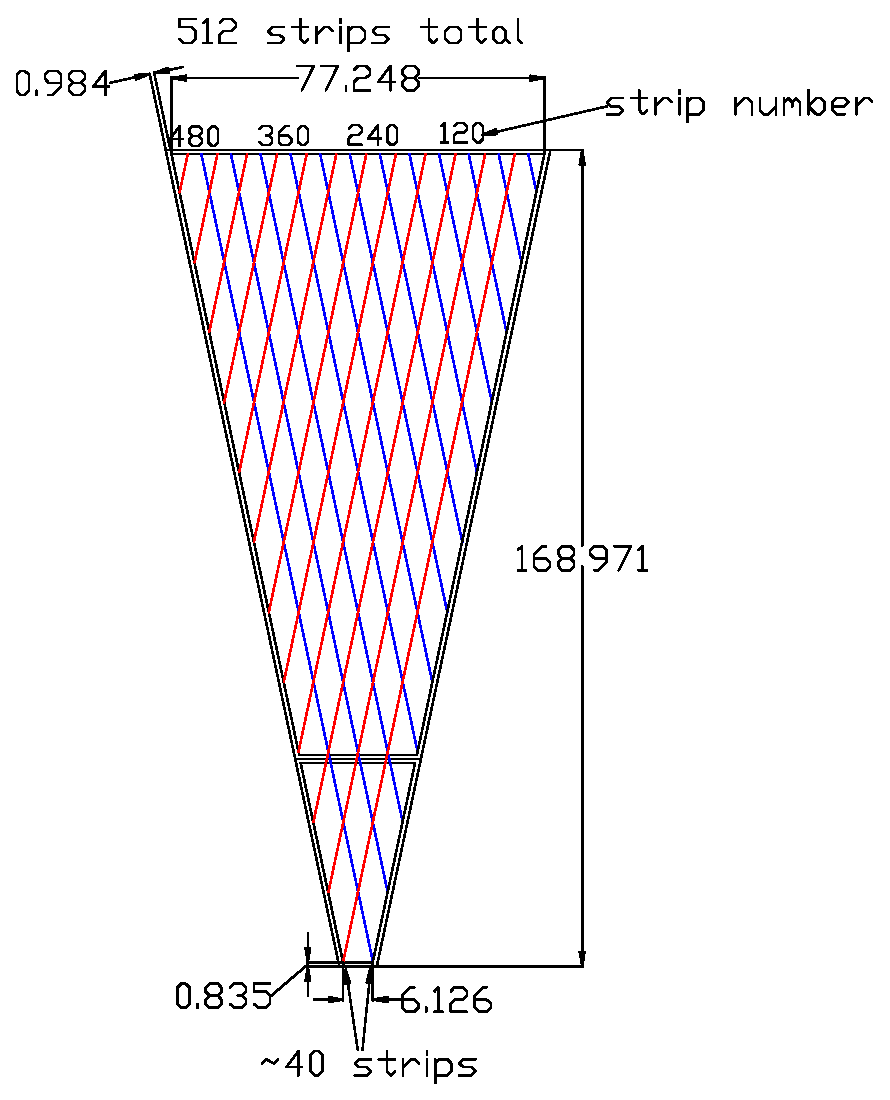
\includegraphics[width=0.6\textwidth]{trap-strip}
\caption{\small{Strip layout for the trapezoidal sensors. All units 
in mm.}}
\label{fig:trap-strip}
\end{figure}
%%%%%%%%%%%%%%%%%%%%%%%%%%%%%%%%%%%%%%%%%%%%%%%%%%%%%%%%%%%%%%%%%%%%%%%

%%%%%%%%%%%%%%%%%%%%%%%%%%%%%%%%%%%%%%%%%%%%%%%%%%%%%%%%%%%%%%%%%%%%%%%
\begin{figure}[htbp]
\centering
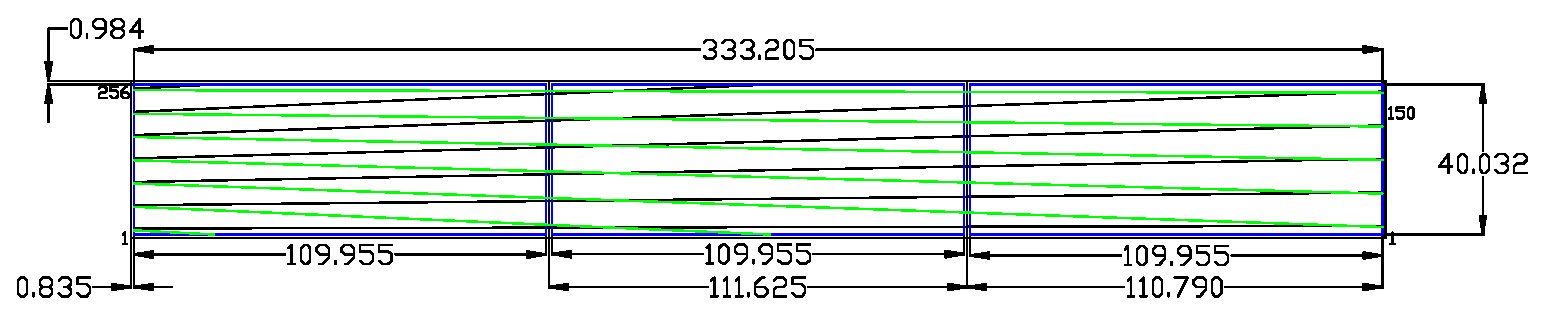
\includegraphics[width=\textwidth]{barrel-strip}
\caption{\small{A standard BST module showing the $V$ and $W$ strips.
All units in mm.}}
\label{barrel_strip}
\end{figure}
%%%%%%%%%%%%%%%%%%%%%%%%%%%%%%%%%%%%%%%%%%%%%%%%%%%%%%%%%%%%%%%%%%%%%%%

\section{Mechanical}

\subsection{Support Structure}

Fig.~\ref{svt_support} shows a view of the complete SVT, including its 
support structure.  A large stainless-steel tube is used to support the BST, 
and the FST is supported off of the BST.   The size and stiffness of the 
support tube seems extreme, but it is a simple system that has been used to 
support other detectors in high magnetic fields in {\tt CLAS} experiments, 
such as the light-weight BONUS detector.   It is expected that the total 
weight of the SVT is less than 10~kg. The calculated deflection of the 
support pipe is 0.033~mm.

%%%%%%%%%%%%%%%%%%%%%%%%%%%%%%%%%%%%%%%%%%%%%%%%%%%%%%%%%%%%%%%%%%%%%%%
\begin{figure}[htbp]
\centering
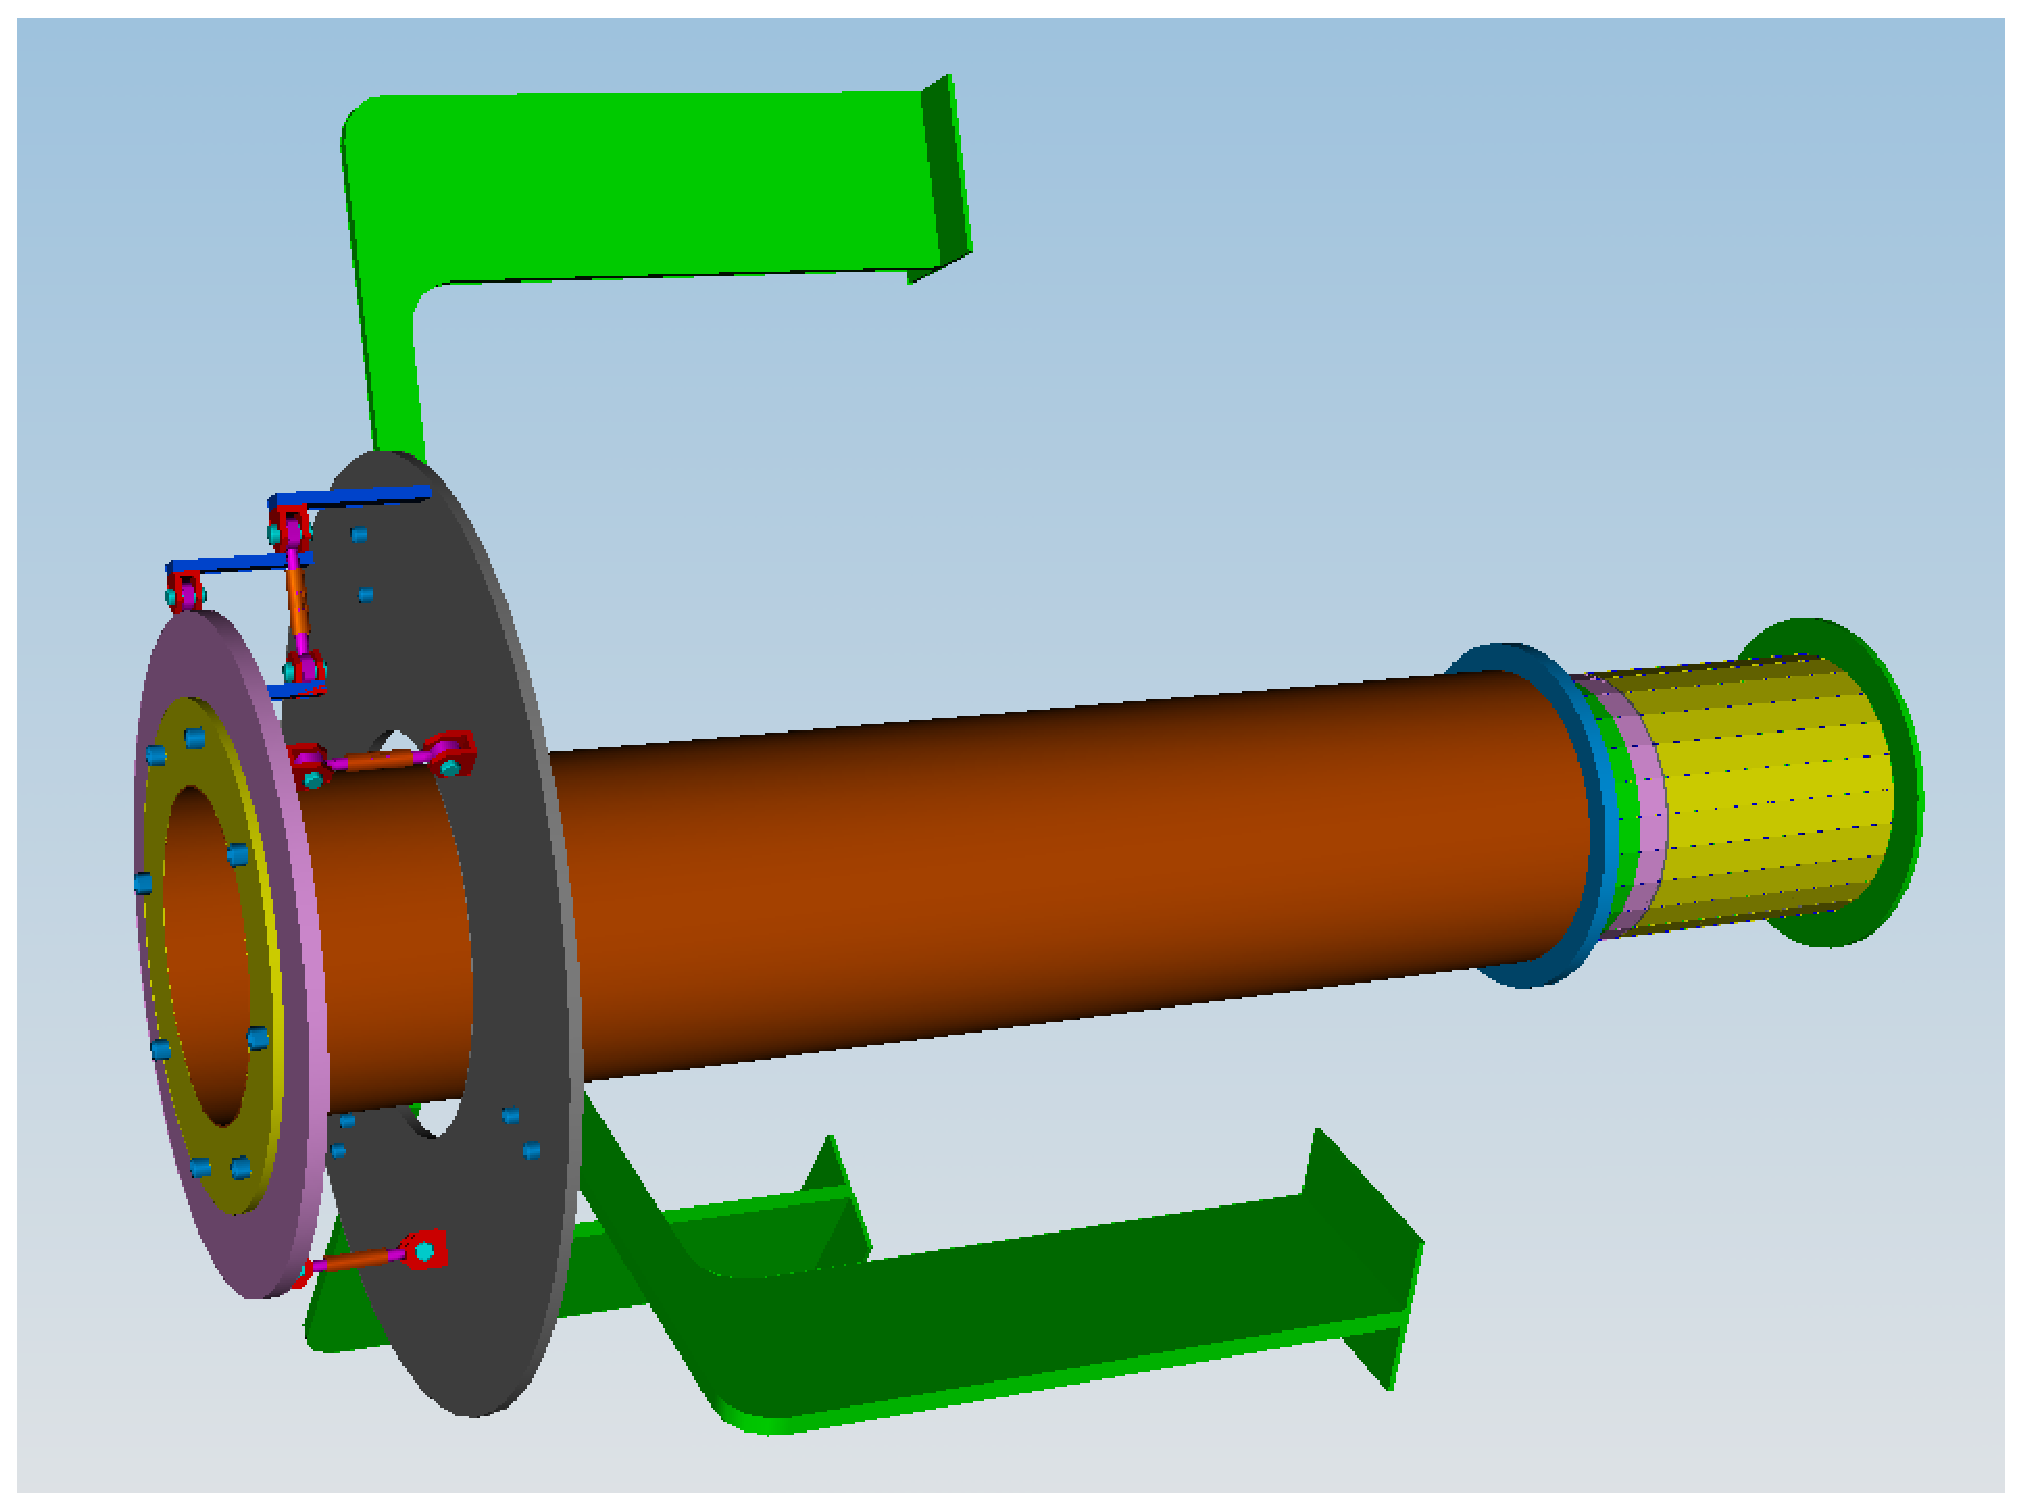
\includegraphics[width=0.60\textwidth]{dave_fig5}
\caption{\small{SVT on support arm with mounting/alignment hardware to
{\tt CLAS12} solenoid.}}
\label{svt_support}
\end{figure}
%%%%%%%%%%%%%%%%%%%%%%%%%%%%%%%%%%%%%%%%%%%%%%%%%%%%%%%%%%%%%%%%%%%%%%%

The relative mass of the support structure is more than 5 times the mass of 
the detector, and it is mounted to the solenoid, which has a mass on the order 
of 20 metric tons, thus vibration will not be an issue.

\subsection{Detector Element Deflection}

Individual staves of the barrel section have been analyzed using ANSYS 
finite element modeling software.  The worst case is Region~1, where its 
deflection is shown in Fig.~\ref{r1_deflect}.  In this modeling, all elements 
of the stave were given both density and stiffness properties, as well as the
dead weight of the electronics (10~g). Deflection of the wafer material can 
be seen to be less than 0.03~mm, which is much less than the required 0.1~mm 
that can cause self induced noise.

%%%%%%%%%%%%%%%%%%%%%%%%%%%%%%%%%%%%%%%%%%%%%%%%%%%%%%%%%%%%%%%%%%%%%%%
\begin{figure}[htbp]
\centering
\includegraphics[width=0.55\textwidth]{dave_ansys1}
\caption{\small{BST Region~1 stave deflection analysis results (units
in mm).}}
\label{r1_deflect}
\end{figure}
%%%%%%%%%%%%%%%%%%%%%%%%%%%%%%%%%%%%%%%%%%%%%%%%%%%%%%%%%%%%%%%%%%%%%%%

\subsection{Detector Element Heat Removal}

Heat removal from the SVT is a significant design issue. The design heat 
load for the SVT is to remove all the on-board electronics heat using 
chilled-water cooling. The total power to be removed is shown in 
Table~\ref{svt_power}.

%%%%%%%%%%%%%%%%%%%%%%%%%%%%%%%%%%%%%%%%%%%%%%%%%%%%%%%%%%%%%%%%%%%%%%%%%
\begin{table}[htbp]
\begin{center}
\begin{tabular} {||l|c|c||} \hline \hline
\multicolumn{3} {|c|} {Heat Load for SVX4}  \\ \hline \hline
Item                       & Barrel & Disk  \\ \hline
No. of modules             & 62     & 45    \\ \hline
Chips/module               & 4      & 8     \\ \hline 
Total chips                & 248    & 360   \\ \hline
Idle power (W)             & 47.6   & 69.1  \\ \hline
Max power/ch (mW/ch)       & 3      & 3     \\ \hline
Max power (W)              & 95.2   & 138.2 \\ \hline
Transceiver power (W)      & 0.5    & 0.5   \\ \hline
No. of transceivers/module & 4      & 4     \\ \hline
Total transceiver power (W)& 124.0  & 90    \\ \hline
Total idle power (W)       & 171.6  & 159.1 \\
(with transceiver)         &        &       \\ \hline
Total max. power (W)       & 219.2  & 228.2 \\
(with transceiver)         &        &       \\ \hline
\end{tabular}
\caption{\small{Heat load on the SVT,}}
\label{svt_power}
\end{center}
\end{table}
%%%%%%%%%%%%%%%%%%%%%%%%%%%%%%%%%%%%%%%%%%%%%%%%%%%%%%%%%%%%%%%%%%%%%%%%%

The primary mode of heat transfer will be conduction heat transfer to a 
water-cooled heat sink.  We have chosen aluminum nitride because it is a 
non-magnetic and electrically non-conductive ceramic material with good 
thermal conductivity.  Two millimeter thick aluminum nitride has been put 
into the core of the staves, replacing the Rohacell core material where 
its mass is not in the acceptance.  Finite element analysis of a Region~4 
module shows that most of the heat can be conducted away, keeping the 
electronics maximum temperature to approximately 40$^\circ$C with the heat 
sink temperature at 15$^\circ$C.  A very small amount of heat (much less 
than 1~W) must be removed from the surface of the wafers to keep them from 
warming to the maximum temperature of the chips.  This can easily be done 
by flushing the detector with a small purge of dry nitrogen.  The temperature 
distribution of a stave in Region~4 is shown in Fig.~\ref{heat_r4}. 

%%%%%%%%%%%%%%%%%%%%%%%%%%%%%%%%%%%%%%%%%%%%%%%%%%%%%%%%%%%%%%%%%%%%%%%
\begin{figure}[htbp]
\centering
\includegraphics[width=0.55\textwidth]{dave_ansys2}
\caption{\small{BST Region~4 stave heat transfer analysis results (units
in $^\circ$C).}}
\label{heat_r4}
\end{figure}
%%%%%%%%%%%%%%%%%%%%%%%%%%%%%%%%%%%%%%%%%%%%%%%%%%%%%%%%%%%%%%%%%%%%%%%

Notice that the temperature along the wafer portion of the stave is around 
23$^\circ$C.  This is because the dry nitrogen that will be purging the 
detector is assumed to be 22$^\circ$C.   Region~1 has a longer conduction 
length, and therefore, higher temperatures are expected.  Two potential 
solutions are being considered.  The first is to use a material with higher 
thermal conductivity (such as a high thermally conductive carbon composite).
The second is to locate the electronics on Region~1 closer to the cooling 
plate.
 
\section{Electronics}

\subsection{Readout}

Both the BST and FST  will be made of single-sided sensors, as single-sided
sensors avoid manufacturing problems and the higher costs associated with
double-sided sensors.  Further, the SVX4 ASIC, a candidate for the readout
electronics, supports single-sided sensors only.  The single-sided sensors
to be used are n-type, AC-coupled, and poly-biased.  After an evaluation of 
the readout ASICs that are available (see Table~\ref{tab:chips}), the 
128-channel SVX4 ASIC that is fabricated on standard 0.25-$\mu$m CMOS 
technology, is considered to be a potential candidate.  SVX4 implements a 
complete readout system and is a low-power device (at 3~mW/channel).  Further, 
the SVX4 ASIC has a good track record and is presently the readout system of 
choice for several single-sided micro-strip detectors.

%%%%%%%%%%%%%%%%%%%%%%%%%%%%%%%%%%%%%%%%%%%%%%%%%%%%%%%%%%%%%%%%%%%%%%%
\begin{table}[htbp]
\begin{center}
\begin{tabular}{|c|c|c|c|c|} \hline
Institution & Experiment & Chip & Manufacturer & Process \\ \hline
CERN & ALICE  & HAL25  & IBM       & 0.25 \\ \hline
CERN & ATLAS  & ABCD   & Honeywell & 0.8  \\ \hline
CERN & CMS    & APV25  & IBM       & 0.25 \\ \hline
CERN & LHCb   & BEETLE & IBM       & 0.25 \\ \hline
FNAL & CDF    & SVX4   & TSMC      & 0.25 \\ \hline
FNAL & D0,CDF & SVX3D  & Honeywell & 0.8  \\ \hline
KEK  & Belle  & VA1TA  & IDEAS     & 0.35 \\ \hline
SLAC & BaBar  & AToM   & Honeywell & 0.8  \\ \hline
\end{tabular}
\end{center}
\caption{\small{Available ASICs that were evaluated for use in {\tt CLAS12}.}}
\label{tab:chips}
\end{table}
%%%%%%%%%%%%%%%%%%%%%%%%%%%%%%%%%%%%%%%%%%%%%%%%%%%%%%%%%%%%%%%%%%%%%%%

As an example of the on-board electronics, a photo-composite of a BST Region~2 
module is shown in Fig.~\ref{fig:module-assembly}.  This assembly is called 
a stave.  Table~\ref{tab:onboard-electronics} lists the significant components 
of the on-detector electronics.  The operating bias voltage is expected to be 
$\sim$200~V.  For low thermal noise and production uniformity, the 
poly-silicon bias resistor is required to be $\sim$2.5~M$\Omega$.  The 
inter-strip resistance is expected to be $\sim$1~G$\Omega$.  To minimize 
signal dispersion, a strip resistance of less than 30~$\Omega$/cm is desirable.

%%%%%%%%%%%%%%%%%%%%%%%%%%%%%%%%%%%%%%%%%%%%%%%%%%%%%%%%%%%%%%%%%%%%%%%
\begin{figure}[htbp]
\centering
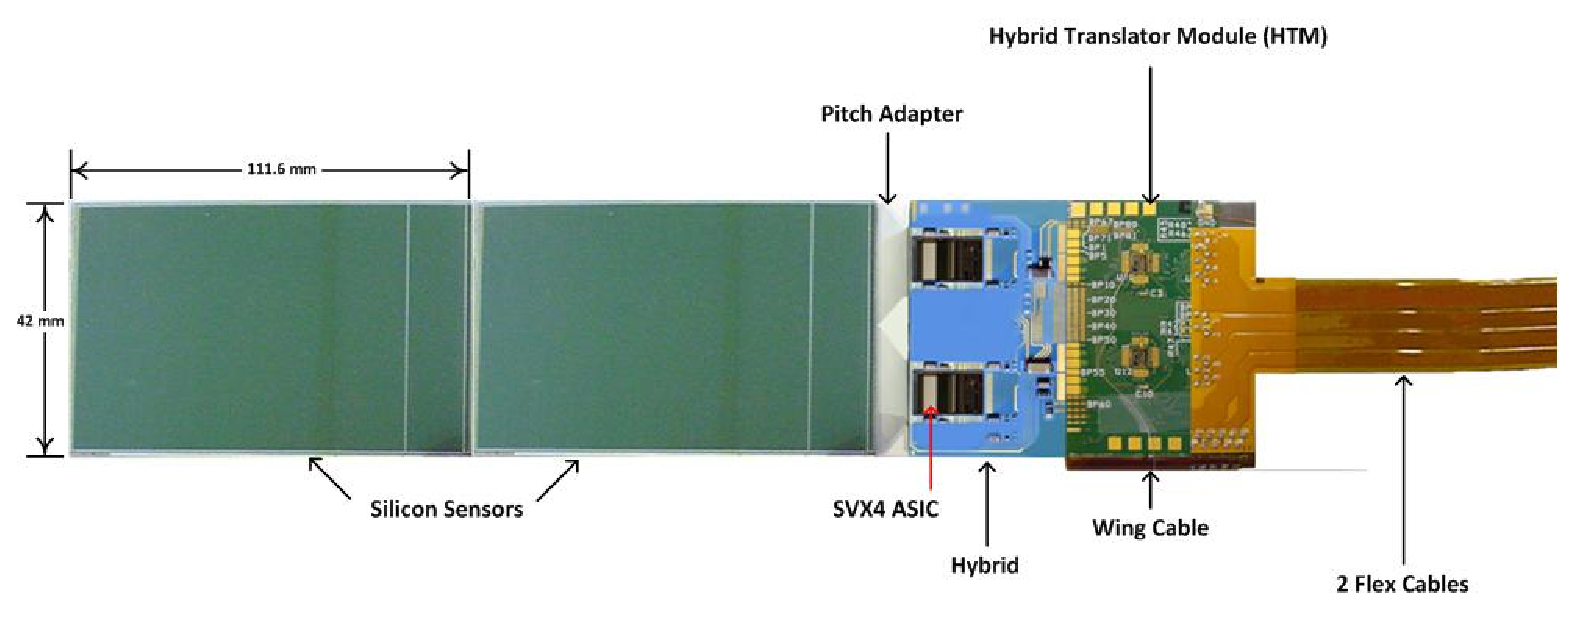
\includegraphics[width=0.85\textwidth]{module-assembly}
\caption{\small{Photo-composite of a Region~2 barrel module stave assembly.}}
\label{fig:module-assembly}
\end{figure}
%%%%%%%%%%%%%%%%%%%%%%%%%%%%%%%%%%%%%%%%%%%%%%%%%%%%%%%%%%%%%%%%%%%%%%%

%%%%%%%%%%%%%%%%%%%%%%%%%%%%%%%%%%%%%%%%%%%%%%%%%%%%%%%%%%%%%%%%%%%%%%%
\begin{table}[htbp]
\begin{center}
\begin{small}
\begin{tabular}{|l|l|l|} \hline
Component       & Basic Specifications & Function \\ \hline
Silicon sensors & Single sided, 300-$\mu$m thick, 42~mm$\times$111.62~mm (cut),
 &   \\
                & 75~$\mu$m implant pitch, 150~$\mu$m readout pitch, $V/W$ & Charge collection \\
                & layers $\pm$1.5$^\circ$, $n$-type, 2 sensors from a 6-in wafer &  \\ \hline
Pitch adapters  & Adapts SVX4 48-$\mu$m pitch to sensor 150-$\mu$m readout 
 & Hybrid to sensor \\
                & pitch       & Connection \\ \hline
Hybrids         & BeO substrate, $\sim$38~mm$\times$20~mm, bonding pads for 
  & SVX4 ASIC mounting\\
                & 2 SVX4 ASICs &  \\ \hline
Hybrid Translator & LVDS signal transceivers, $\sim$40~mm$\times$40~mm 
(smaller & Translates and repeats \\
Module (HTM)    & if possible)            & module control and \\
                &                         & data signals \\ \hline
Wing cable & Flex cable extension of HTM circuit board, & Connects signals from \\
                & wire-bond pads for bottom hybrid & top to bottom HTM \\ \hline
\end{tabular}
\end{small}
\end{center}
\caption{\small{Significant components of the on-board electronics.}}
\label{tab:onboard-electronics}
\end{table}
%%%%%%%%%%%%%%%%%%%%%%%%%%%%%%%%%%%%%%%%%%%%%%%%%%%%%%%%%%%%%%%%%%%%%%%

The SVX4 design handles sensor capacitances from 10~pF to 35~pF.  For the
FST and the BST, the total inter-strip capacitance is expected to be
$\le$1.2~pF/cm and the coupling capacitance is expected to be
$\ge$10~pF/cm for AC-coupled strips.  The equivalent noise charge (ENC) in 
a channel is given by ENC = $400 e^- + 42 e^-/$~pF.  For a capacitance of 
30~pF, the typical capacitance of a long strip, plus some additional stray 
capacitance due to the wire-bonds connecting the sensor and the chip, ENC 
is estimated to be 1800$e^-$.  This noise level is about a tenth of the 
signal level generated by a minimum ionizing particle.

Fig.~\ref{fig:svx-channel-sch} shows a block diagram of a single SVX4 
channel.  The detector signals are integrated, correlated double samples, 
the difference of which is stored in the analog pipeline.  Up to 42 
measurements can be stored in the pipeline.  Digitization is by means of a 
Wilkinson-type ADC and an 8-bit counter.  Timing control signals govern, 
among other functions, the operation of each channel's preamp reset, the 
double-correlated sampling, and the ADC.  These timing control signals must 
be generated by a trigger generated by other detectors in {\tt CLAS12}.
Once a pipeline cell is marked by the Level-1 accept (L1A) trigger, the 
counter value is stored in a FIFO buffer.  An 8-bit output bus transmits 
the data in a sequence of bytes identifying the chip, pipeline cell, the 
channel number, and the content.

%%%%%%%%%%%%%%%%%%%%%%%%%%%%%%%%%%%%%%%%%%%%%%%%%%%%%%%%%%%%%%%%%%%%%%%
\begin{figure}[htbp]
\vspace{5.7cm}
\special{psfile=svx-channel-sch.eps hscale=55 vscale=55 
hoffset=40 voffset=-5}
\caption{\small{Schematic of an SVX4 chip showing the layout for the
preamp, through the pipeline and ADC to the FIFO buffer.}}
\label{fig:svx-channel-sch}
\end{figure}
%%%%%%%%%%%%%%%%%%%%%%%%%%%%%%%%%%%%%%%%%%%%%%%%%%%%%%%%%%%%%%%%%%%%%%%

%%%%%%%%%%%%%%%%%%%%%%%%%%%%%%%%%%%%%%%%%%%%%%%%%%%%%%%%%%%%%%%%%%%%%%%
\begin{figure}[htbp]
\centering
\includegraphics[width=0.5\textwidth]{svx-floorplan}
\caption{\small{SVX4 ASIC floor plan.}}
\label{fig:svx-floorplan}
\end{figure}
%%%%%%%%%%%%%%%%%%%%%%%%%%%%%%%%%%%%%%%%%%%%%%%%%%%%%%%%%%%%%%%%%%%%%%%

Fig.~\ref{fig:svx-floorplan} shows the floor plan of the SVX4 ASIC.
The thickness of the chip is 0.25~mm.  The diced area of the chip is 
6.40~mm $\times$ 9.11~mm.  The channel input pads are 0.096~mm apart, 
center-to-center, and the pad widths are 0.048~mm.  There are two rows 
of input pads to which the outputs of the silicon sensors have to be 
wire-bonded.  Pitch adapters connect the sensor and the hybrid.  Wire-bond 
pads are located on both ends of the pitch adapter for connections to the 
SVX4 ASICs and to the sensor.  The wire-bonding pads will be compatible 
with the aluminum-wire ultrasonic wedge-bonding method.  A separate ceramic
pitch adapter will be glued onto the module support assembly.
Fig.~\ref{fig:pitch-adapter} shows the pitch adapter connections to the 
sensor and SVX4 ASICs.  Fiducial marks will be made on the pitch adapter
for assembly and alignment.  In addition to routing the sensor signals and 
the guard ground, the high voltage will be routed across the pitch adapter 
from the hybrid to the sensor bias ring.  Adequate spacing between the pitch 
adapter, high voltage trace, sensor guard, and ground will be provided.

%%%%%%%%%%%%%%%%%%%%%%%%%%%%%%%%%%%%%%%%%%%%%%%%%%%%%%%%%%%%%%%%%%%%%%%
\begin{figure}[htbp]
\centering
\includegraphics[width=0.65\textwidth]{pitch-adapter}
\caption{\small{Pitch adapter connections to the sensor.}}
\label{fig:pitch-adapter}
\end{figure}
%%%%%%%%%%%%%%%%%%%%%%%%%%%%%%%%%%%%%%%%%%%%%%%%%%%%%%%%%%%%%%%%%%%%%%%

Fig.~\ref{fig:hybrid} shows a photo-composite of the proposed hybrid for
mounting the SVX4 chips.  The hybrid will be outside of the active area, 
not on the sensor, and glued directly onto the support structure.  The 
proposed hybrid with approximate dimensions of 38~mm $\times$ 20~mm will 
be used to mount the two SVX4 readout ASICs.  The hybrid substrate uses 
beryllium oxide, which is a good heat conductor and has a long radiation 
length.  The gold bond pads of the hybrid will be aluminum-wedge bondable 
to be compatible with the other components.  The high voltage for the 
sensors will be routed across the hybrid with an adequate wire-bonding 
surface for connections to the pitch adapter and the hybrid translator 
module (HTM).  An RTD (resistance temperature detector) will be mounted 
on the hybrid for temperature measurements.

%%%%%%%%%%%%%%%%%%%%%%%%%%%%%%%%%%%%%%%%%%%%%%%%%%%%%%%%%%%%%%%%%%%%%%%
\begin{figure}[htbp]
\centering
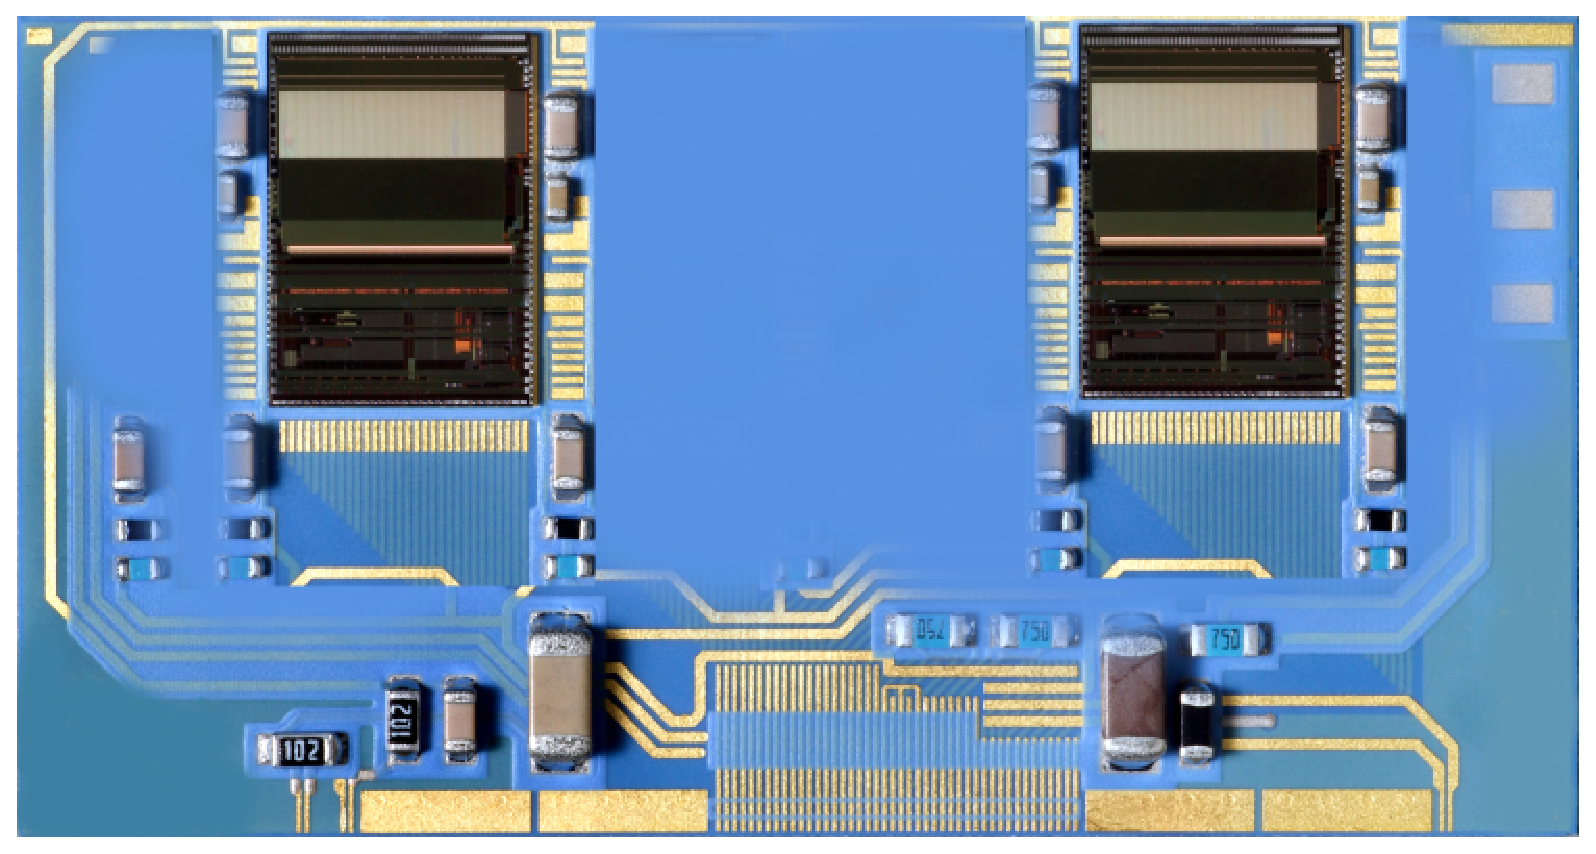
\includegraphics[width=0.5\textwidth]{hybrid}
\caption{\small{Photo-composite of the hybrid board for mounting of the
SVX4 chips.}}
\label{fig:hybrid}
\end{figure}
%%%%%%%%%%%%%%%%%%%%%%%%%%%%%%%%%%%%%%%%%%%%%%%%%%%%%%%%%%%%%%%%%%%%%%%

Separate power supplies and grounds for the analog and digital sections 
will be used.  The dielectric strength of the circuit board will be 
$\geq$650~V/mil.  SVX4 diagnostic signals have external pull-up resistors 
and will be routed to the hybrid test points.  Fig.~\ref{fig:hybrid-sch} 
shows a conceptual schematic of the hybrid based on the FNAL CDF design.

%%%%%%%%%%%%%%%%%%%%%%%%%%%%%%%%%%%%%%%%%%%%%%%%%%%%%%%%%%%%%%%%%%%%%%%
\begin{figure}[htbp]
\centering
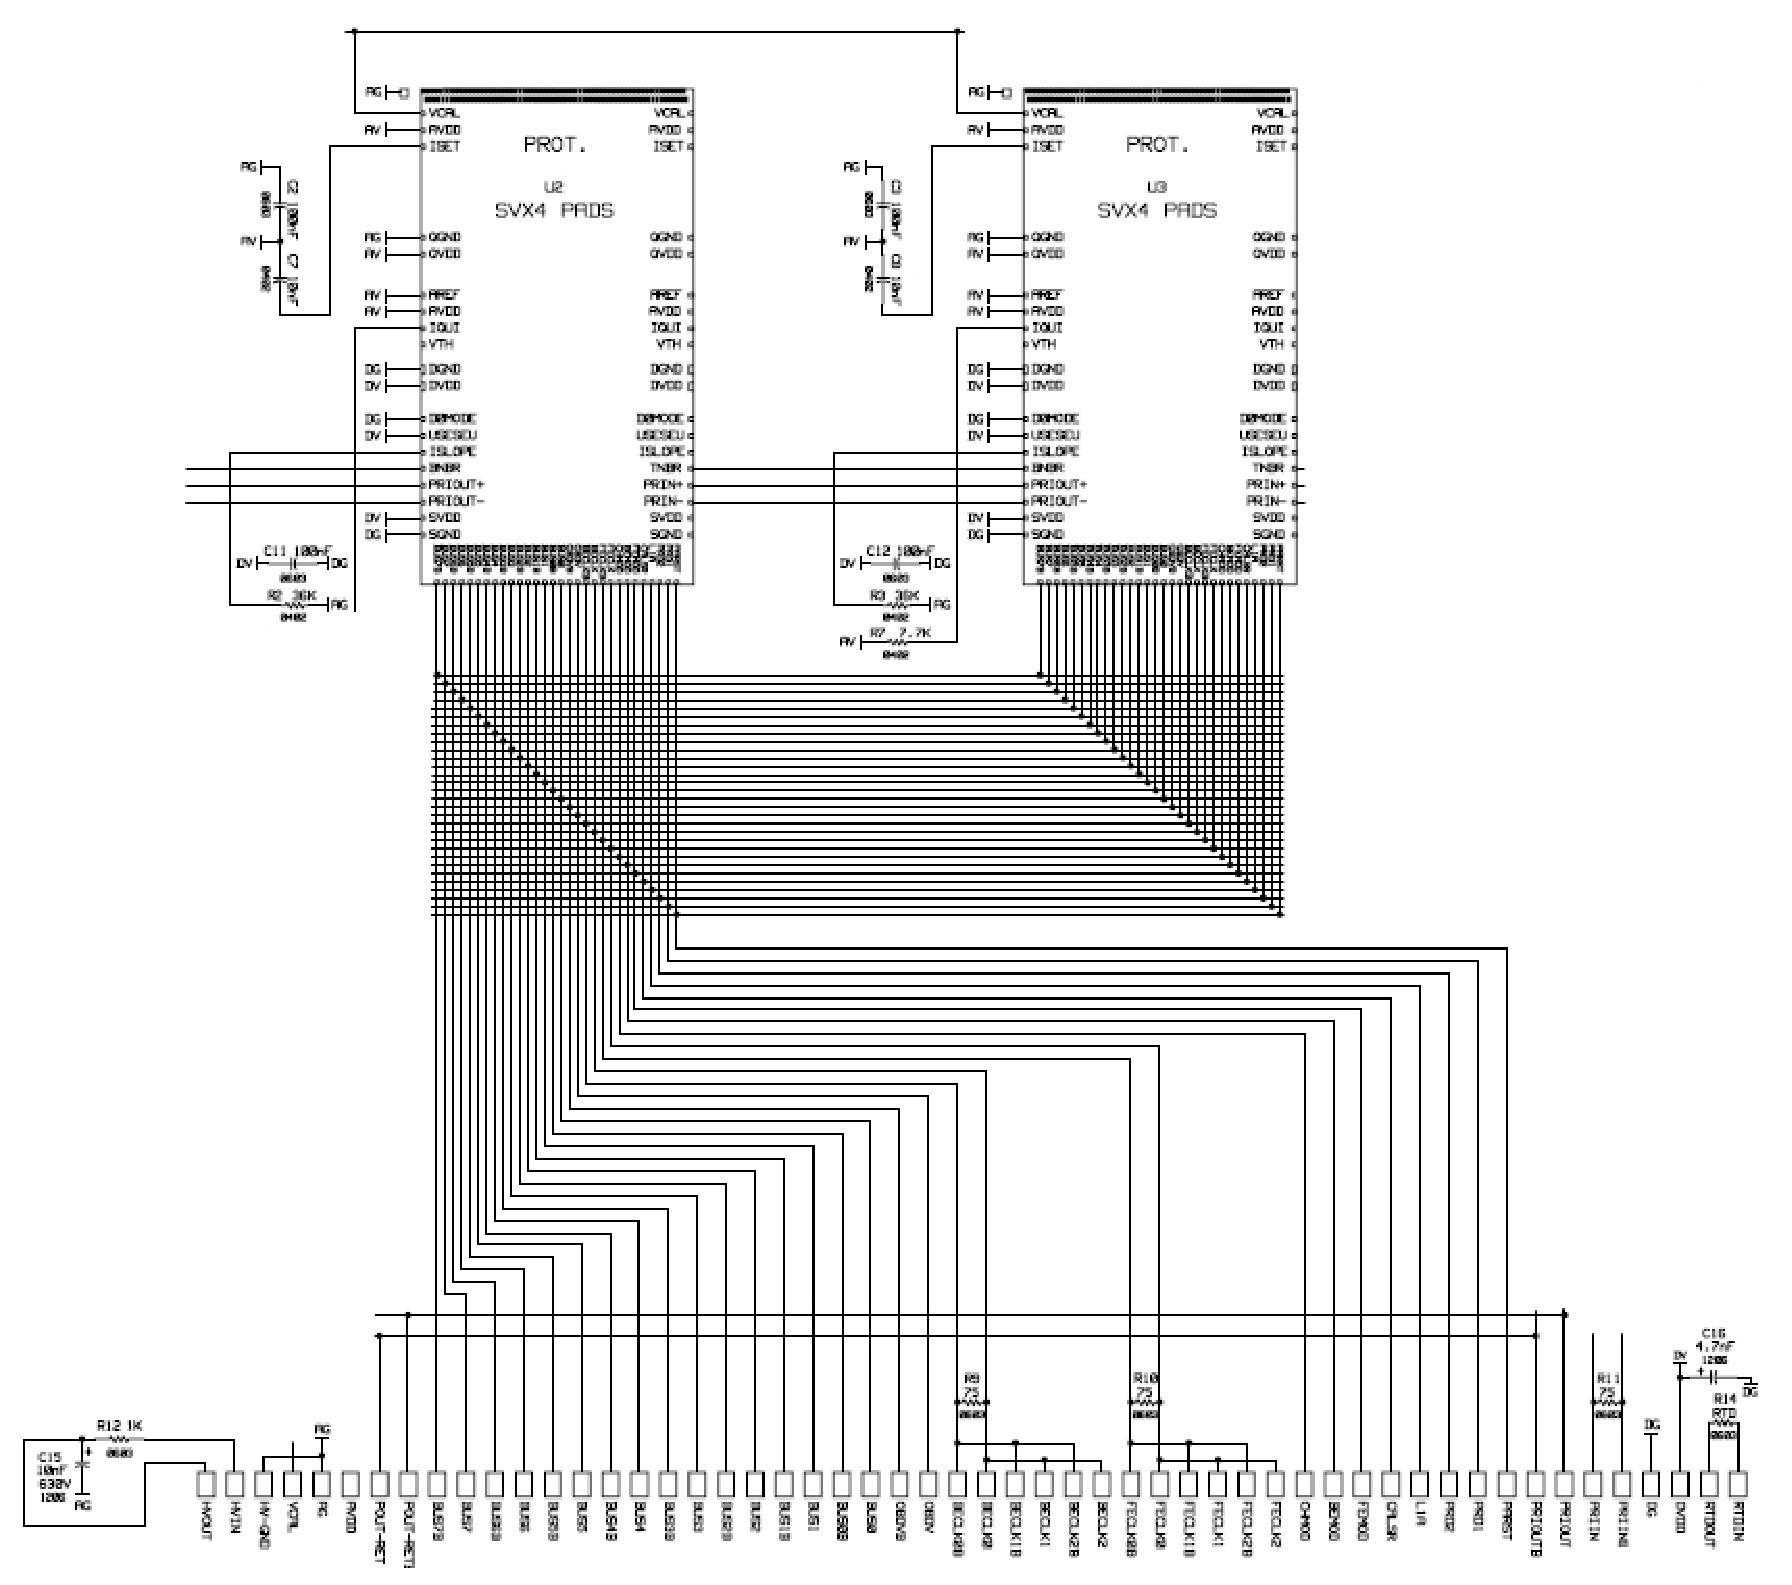
\includegraphics[width=0.9\textwidth]{hybrid-sch}
\caption{\small{Conceptual schematic of the hybrid board layout of the
SVT.}}
\label{fig:hybrid-sch}
\end{figure}
%%%%%%%%%%%%%%%%%%%%%%%%%%%%%%%%%%%%%%%%%%%%%%%%%%%%%%%%%%%%%%%%%%%%%%%

The connections for the priority in - priority out SVX4 readout chain 
allow for reading the top side and then the bottom side of the module.
The input and output for the readout chain are then routed to HTM 
transceivers and then to the external connectors.  The HTM translates and 
repeats control and data signals from the two hybrids on a module to the 
DAQ.  The HTM also routes the low voltage and high voltage supply lines 
from the flex cables to the hybrid.  Fig.~\ref{fig:readout-chain} shows a 
conceptual block diagram of the SVX4 readout chain.  Fig.~\ref{htm} (top) 
shows a FNAL HTM that has the dimensions of 39~mm $\times$ 50~mm; at JLab 
a smaller module ($\sim$40~mm $\times$ 30~mm or less) is being developed 
for {\tt CLAS12}.  Fig.~\ref{htm} (bottom) shows a block diagram of the 
HTM board.  The FNAL 10-bit low voltage differential signal ASIC 
transceiver will be used because of its high density and its good track 
record with silicon-strip detectors.  The transceiver comes in die form 
and is wire-bonded to the HTM board.

%%%%%%%%%%%%%%%%%%%%%%%%%%%%%%%%%%%%%%%%%%%%%%%%%%%%%%%%%%%%%%%%%%%%%%%
\begin{figure}[htbp]
\centering
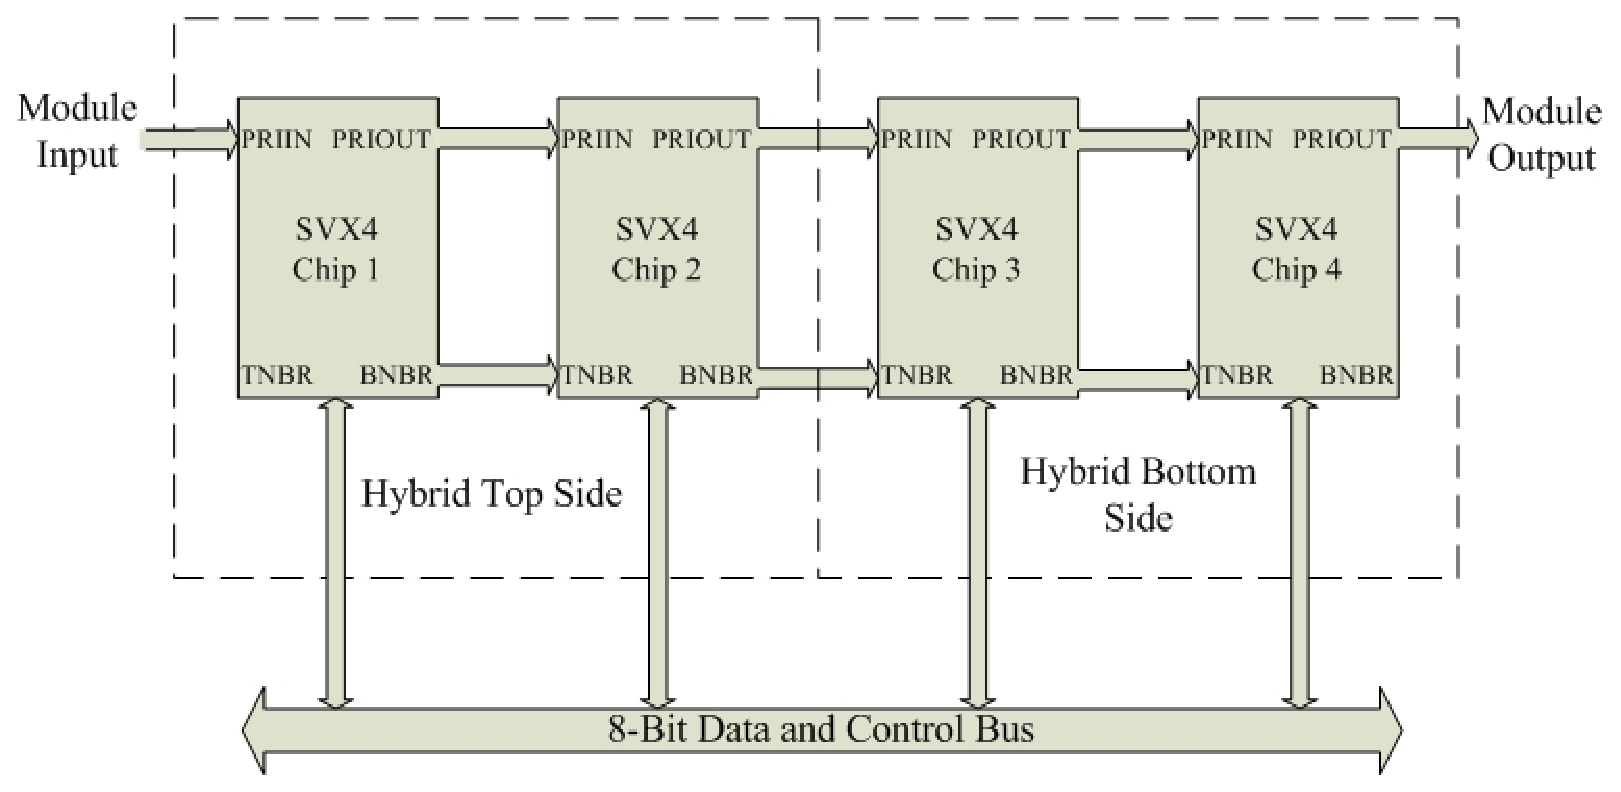
\includegraphics[width=0.75\textwidth]{readout-chain}
\caption{\small{SVX4 readout chain configuration.}}
\label{fig:readout-chain}
\end{figure}
%%%%%%%%%%%%%%%%%%%%%%%%%%%%%%%%%%%%%%%%%%%%%%%%%%%%%%%%%%%%%%%%%%%%%%%

%%%%%%%%%%%%%%%%%%%%%%%%%%%%%%%%%%%%%%%%%%%%%%%%%%%%%%%%%%%%%%%%%%%%%%%
\begin{figure}[htbp]
\vspace{13.5cm}
\special{psfile=htm-top.eps hscale=45 vscale=45 hoffset=20 voffset=235}
\special{psfile=htm-sch.eps hscale=40 vscale=40 hoffset=210 voffset=0}
\caption{\small{(Top) Top side view of the hybrid translator module (HTM).
(Bottom) Corresponding block diagram for the HTM board.}}
\label{htm}
\end{figure}
%%%%%%%%%%%%%%%%%%%%%%%%%%%%%%%%%%%%%%%%%%%%%%%%%%%%%%%%%%%%%%%%%%%%%%%

The ``wing'' cable connects the bottom-side hybrid to the transceiver on 
the HTM board.  The wing cable and the HTM will be combined together into 
a single polyimide rigid (HTM) and flex (wing cable) assembly.  In addition 
to the wing cable, the two flex cables with the data, low voltage, and high 
voltage connectors will be attached to the HTM board.  
Fig.~\ref{fig:wing-cable} shows the wing cable on bottom side of the module.  
Fig.~\ref{fig:htm} shows the HTM board and wing cable before folding.
Fig.~\ref{fig:flex-cable} shows the flex cable assembly.  The length of 
the cable is limited to $\sim$30~cm.  Fig.~\ref{routing} shows the flow of 
the cables.  All cables will be routed to the electronic racks located at 
the rear of the detector.

%%%%%%%%%%%%%%%%%%%%%%%%%%%%%%%%%%%%%%%%%%%%%%%%%%%%%%%%%%%%%%%%%%%%%%%
\begin{figure}[htbp]
\centering
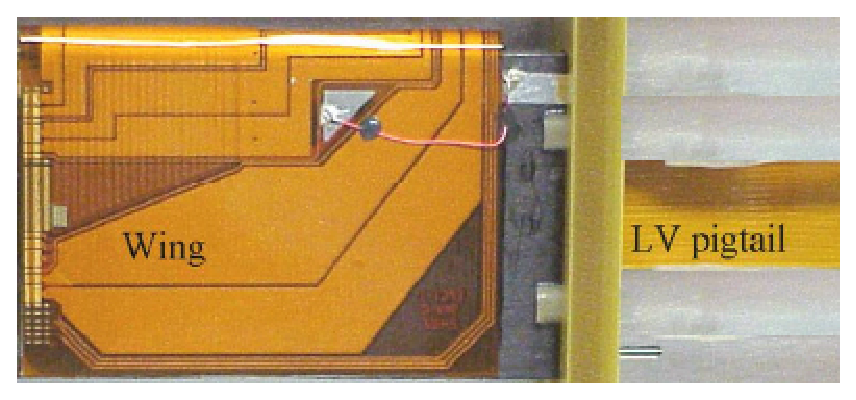
\includegraphics[width=0.65\textwidth]{wing-cable}
\caption{\small{Wing cable on the bottom of the HTM board.}}
\label{fig:wing-cable}
\end{figure}
%%%%%%%%%%%%%%%%%%%%%%%%%%%%%%%%%%%%%%%%%%%%%%%%%%%%%%%%%%%%%%%%%%%%%%%

%%%%%%%%%%%%%%%%%%%%%%%%%%%%%%%%%%%%%%%%%%%%%%%%%%%%%%%%%%%%%%%%%%%%%%%
\begin{figure}[htbp]
\centering
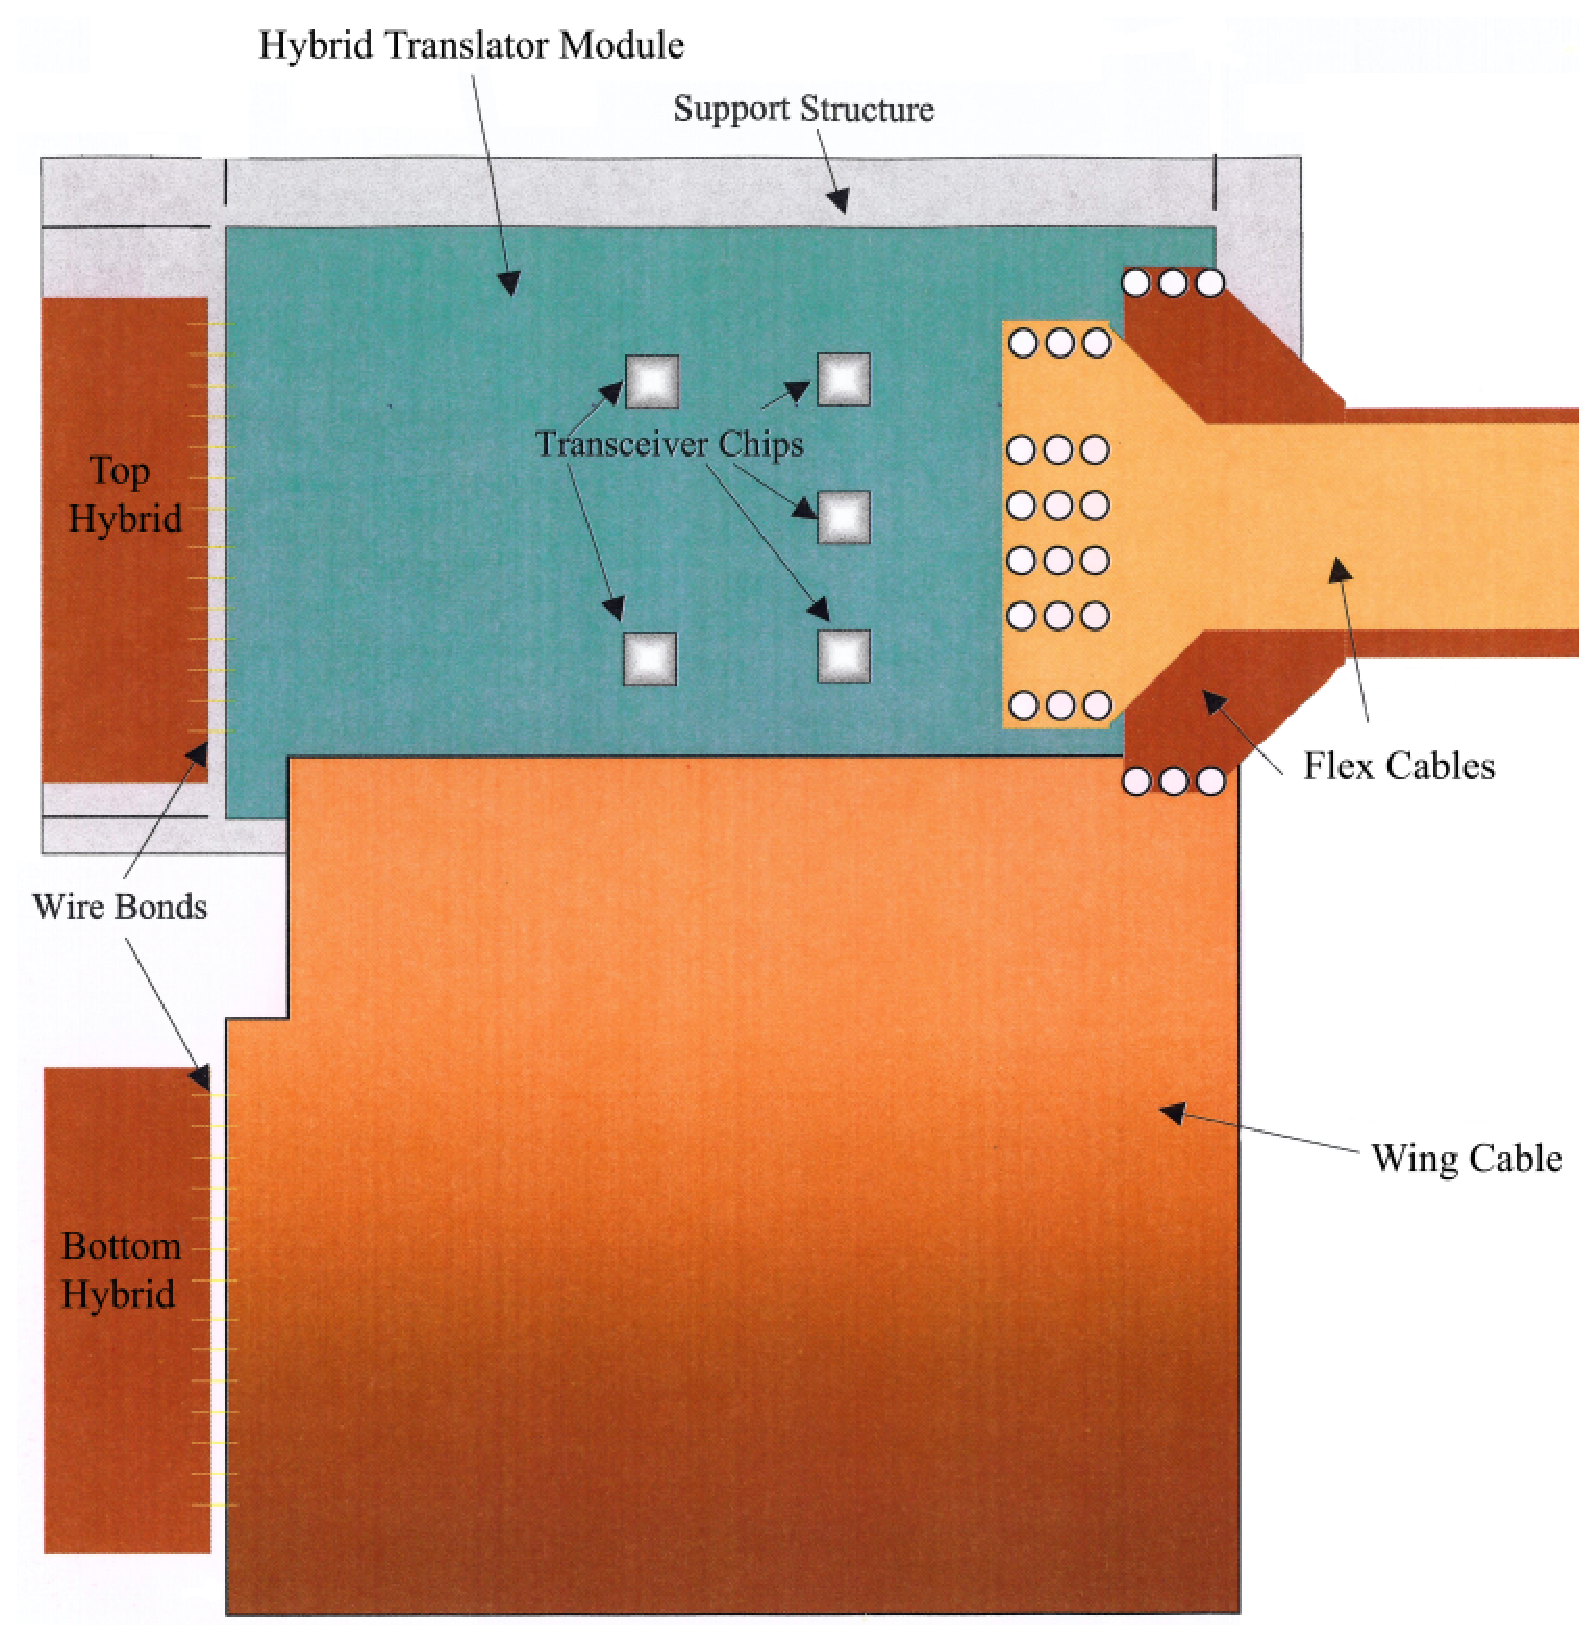
\includegraphics[width=0.5\textwidth]{htm}
\caption{\small{HTM assembly showing the wing cable to connect the top
and bottom side boards and the readout flex cable.}}
\label{fig:htm}
\end{figure}
%%%%%%%%%%%%%%%%%%%%%%%%%%%%%%%%%%%%%%%%%%%%%%%%%%%%%%%%%%%%%%%%%%%%%%%

%%%%%%%%%%%%%%%%%%%%%%%%%%%%%%%%%%%%%%%%%%%%%%%%%%%%%%%%%%%%%%%%%%%%%%%
\begin{figure}[htbp]
\centering
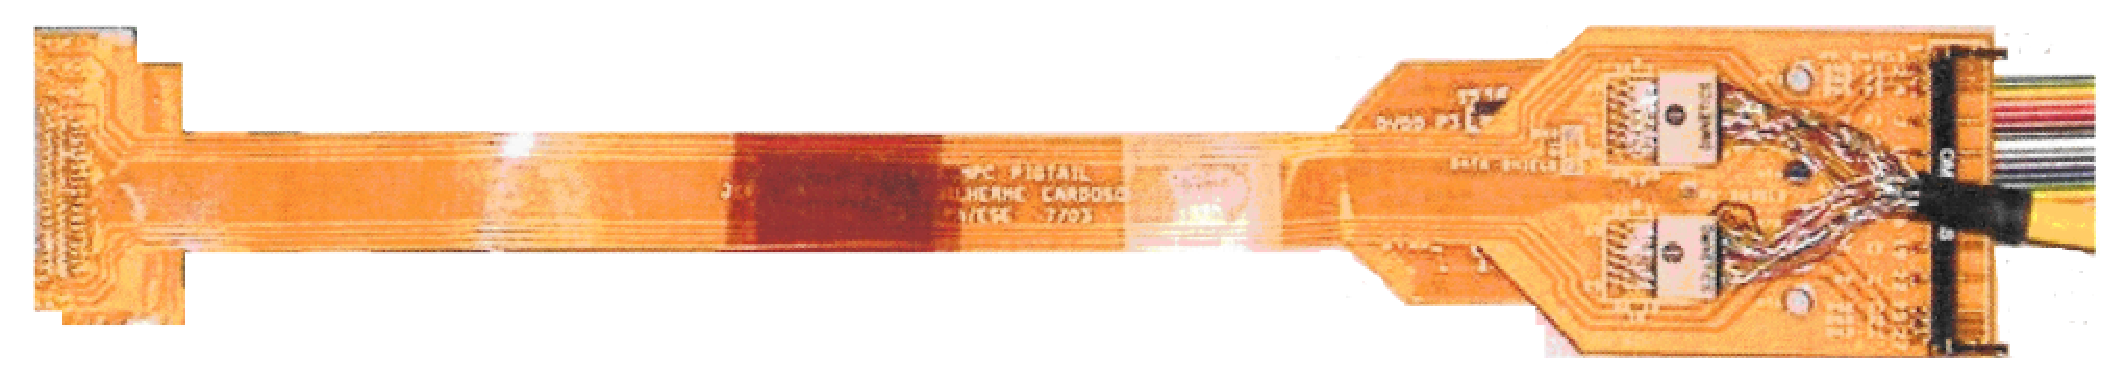
\includegraphics[width=\textwidth]{flex-cable}
\caption{\small{Photograph of the flex cable assembly.}}
\label{fig:flex-cable}
\end{figure}
%%%%%%%%%%%%%%%%%%%%%%%%%%%%%%%%%%%%%%%%%%%%%%%%%%%%%%%%%%%%%%%%%%%%%%%

%%%%%%%%%%%%%%%%%%%%%%%%%%%%%%%%%%%%%%%%%%%%%%%%%%%%%%%%%%%%%%%%%%%%%%%
\begin{figure}[htbp]
\vspace{8.5cm}
\special{psfile=cable-route.eps hscale=22 vscale=22 hoffset=85 
voffset=10}
\caption{\small{Cable routing diagram for the SVT detector.}}
\label{routing}
\end{figure}
%%%%%%%%%%%%%%%%%%%%%%%%%%%%%%%%%%%%%%%%%%%%%%%%%%%%%%%%%%%%%%%%%%%%%%%

\subsection{High and Low Voltage}

The system is designed with the highest low voltage and high voltage 
segmentation affordable, without compromising performance and operability.
Each side of the module has its own high voltage channel, two high voltage 
channels per module.  The five channels of low voltage for the module 
consist of a hybrid analog and a hybrid digital channel for the top and 
for the bottom sides of the sensor module and a digital channel for the HTM.
All of these channels operate at 2.5~V.  In addition to the low voltage and 
high voltage, a calibration voltage for each of the two hybrids connects to 
the flex cable low voltage connector.

The low voltage system consists of $\sim$625 channels in four groups.  The 
high voltage system has $\sim$240 channels.  Fig.~\ref{fig:system-connections}
shows the distribution of voltage and monitoring channels for the SVT.  The 
low voltage and high voltage supplies for the SVT will be modular with 
individual channels provided by a module within a main supply crate.  
Sensors will have a controllable and monitorable high voltage channel with 
over-current and over-voltage trip protection.  A calibration signal and a 
temperature sensor on each hybrid will be instrumented on the detector 
modules.  Table~\ref{tab:voltages} shows the distribution of low and high 
voltage channels needed for the sensors, the HTMs, and the sector collector 
modules (SCM). 

%%%%%%%%%%%%%%%%%%%%%%%%%%%%%%%%%%%%%%%%%%%%%%%%%%%%%%%%%%%%%%%%%%%%%%%
\begin{table}[htbp]
\begin{center}
\begin{small}
\begin{tabular}{|c|c|c|c|c|c|} \hline
Specification & Region 1 & Region 2 & Region 3 & Region 4 & Total \\ \hline
Hybrid 2.5 V digital channels (barrel) & 14 & 24 & 34 & 44 & 116 \\ \hline
Hybrid 2.5 V digital channels (nose cone) & 40 & 42 & 42 & 0 & 124 \\ \hline
Hybrid 2.5 V analog channels (barrel) & 14 & 24 & 34 & 44 & 116 \\ \hline
Hybrid 2.5 V analog channels (nose cone) & 40 & 42 & 42 & 0 & 124 \\ \hline
HTM LV channels (barrel) & 7 & 12 & 17 & 22 & 58 \\ \hline
HTM LV channels (nose cone) & 20 & 21 & 21 & 0 & 62 \\ \hline
SCM LV channels (barrel) & 2 & 3 & 4 & 4 & 13 \\ \hline
SCM LV channels (nose cone) & 4 & 5 & 5 & 0 & 14 \\ \hline
HV channels (barrel) & 14 & 24 & 34 & 44 & 116 \\ \hline
HV channels (nose cone) & 40 & 42 & 42 & 0 & 124 \\ \hline \hline
\end{tabular}
\end{small}
\end{center}
\caption{\small{High and low voltage channel distribution for the SVT.}}
\label{tab:voltages}
\end{table}
%%%%%%%%%%%%%%%%%%%%%%%%%%%%%%%%%%%%%%%%%%%%%%%%%%%%%%%%%%%%%%%%%%%%%%%

The CAEN crate-based high voltage systems, including the 1527 and 1527LC, 
and the WIENER universal multi-channel modular system for both low voltage 
and high voltage supply are being considered.  The WIENER modular system 
has the advantage of a common crate that will support both high voltage 
and low voltage modules.  Fig.~\ref{fig:system-connections} shows an 
overview of the connections of the system.

%%%%%%%%%%%%%%%%%%%%%%%%%%%%%%%%%%%%%%%%%%%%%%%%%%%%%%%%%%%%%%%%%%%%%%%
\begin{figure}[htbp]
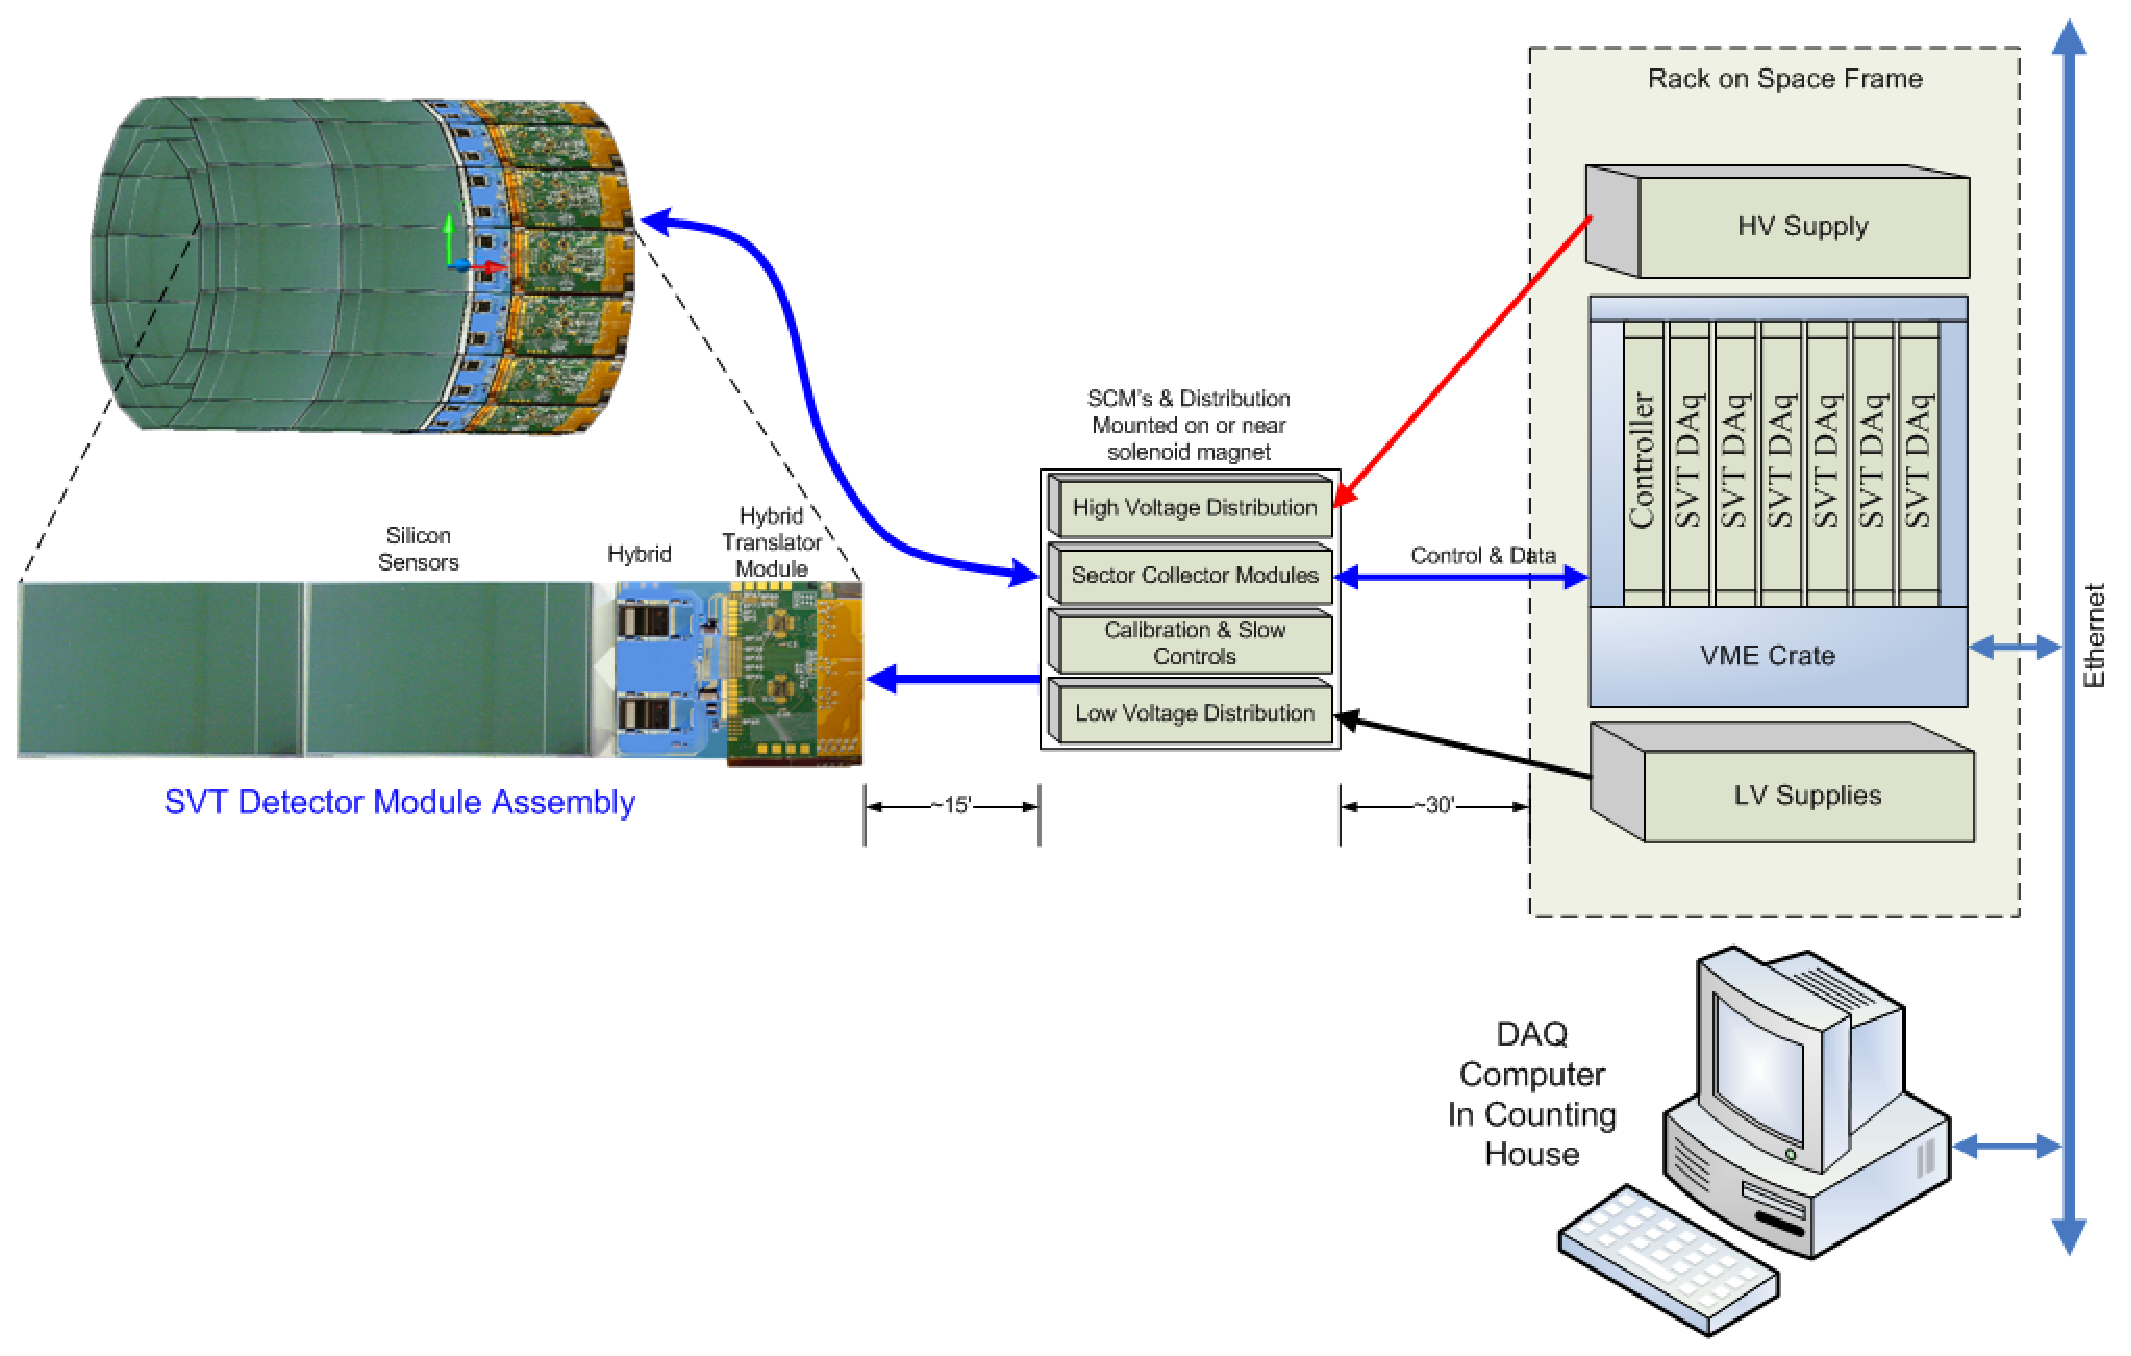
\includegraphics[width=0.9\textwidth]{system-connections}
\caption{\small{System connections overview for the SVT.}}
\label{fig:system-connections}
\end{figure}
%%%%%%%%%%%%%%%%%%%%%%%%%%%%%%%%%%%%%%%%%%%%%%%%%%%%%%%%%%%%%%%%%%%%%%%

\subsection{Slow Controls}

Calibration and testing of the detector modules and readout chain is 
accomplished by a calibration input signal (VCAL).  This external input 
on each SVX4 ASIC has the capability of injecting a small charge via a  
charge injection capacitor (25~fF).  This capacitor can be switched in 
from each preamp input to a common bus line.  A 128-bit programmable 
channel register, downloaded in the initialize mode, can function as a 
mask register and determine whether or not the injection capacitor is 
switched on for each channel.  Fig.~\ref{fig:svx-block} (left) shows the 
preamp stage of the SVX4 ASIC and the VCAL calibration input.

The slow controls system (SCS) will be responsible for controlling all 
essential run-time parameters of the experiment and for monitoring the 
status of various hardware components.  The primary goals are to enhance 
safety by providing early warnings about malfunctioning equipment and check 
the health of the experiment and the integrity of data.  The system will 
also transmit important parameters to the DAQ for insertion in the 
{\tt CLAS12} data stream.  The SCS will have the ability to trigger alarms 
to notify personnel when parameters are detected to be outside pre-defined 
limits and will have the option of automatically disabling DAQ in case of 
a severe malfunction of the equipment.  The implementation of the SCS will 
need a VME crate with an IOC and input/output boards.  Some of the hardware 
will be connected directly to the Ethernet network.  The settings of all 
critical operating parameters will be protected against computer failure.  
The failure of the computer in the system will only result in the loss of 
monitoring.  When a computer reboots, parameters will not reset to 
previous or default values but remain at currently set values.

The SVT computers and vital support hardware will be protected by 
Uninterruptible Power Supplies (UPS) with battery backup and software to 
signal an alarm and notify the operators when external power is lost.
The UPS will have surge protection and line filtering.  Monitoring and 
control of the system will be implemented through the use of a Motorola 
single board computer embedded in a VME crate running VXworks real-time 
operating system.  Sun or Hewlett-Packard workstations will support the 
user interfaces and controls.  The control software will be built using 
the toolkit provided by the Experimental Physics and Industrial Control 
System (EPICS), which is based on the client-server model.

\subsection{Data Acquisition}
\label{svt:daq}

Each channel of the SVX4 ASIC has a 42-cell deep analog pipeline.
Fig.~\ref{fig:svx-block} shows the block diagram of the ASIC.  The 
front-end of the ASIC contains the integrator and storage pipeline, which 
at a front end clock rate (FEClk) of 132~ns, allows a trigger latency of 
$\sim$4~$\mu$s.  The back-end of the ASIC has an ADC for digitization and 
the readout and driver logic.

%%%%%%%%%%%%%%%%%%%%%%%%%%%%%%%%%%%%%%%%%%%%%%%%%%%%%%%%%%%%%%%%%%%%%%%
\begin{figure}[htbp] 
\centering
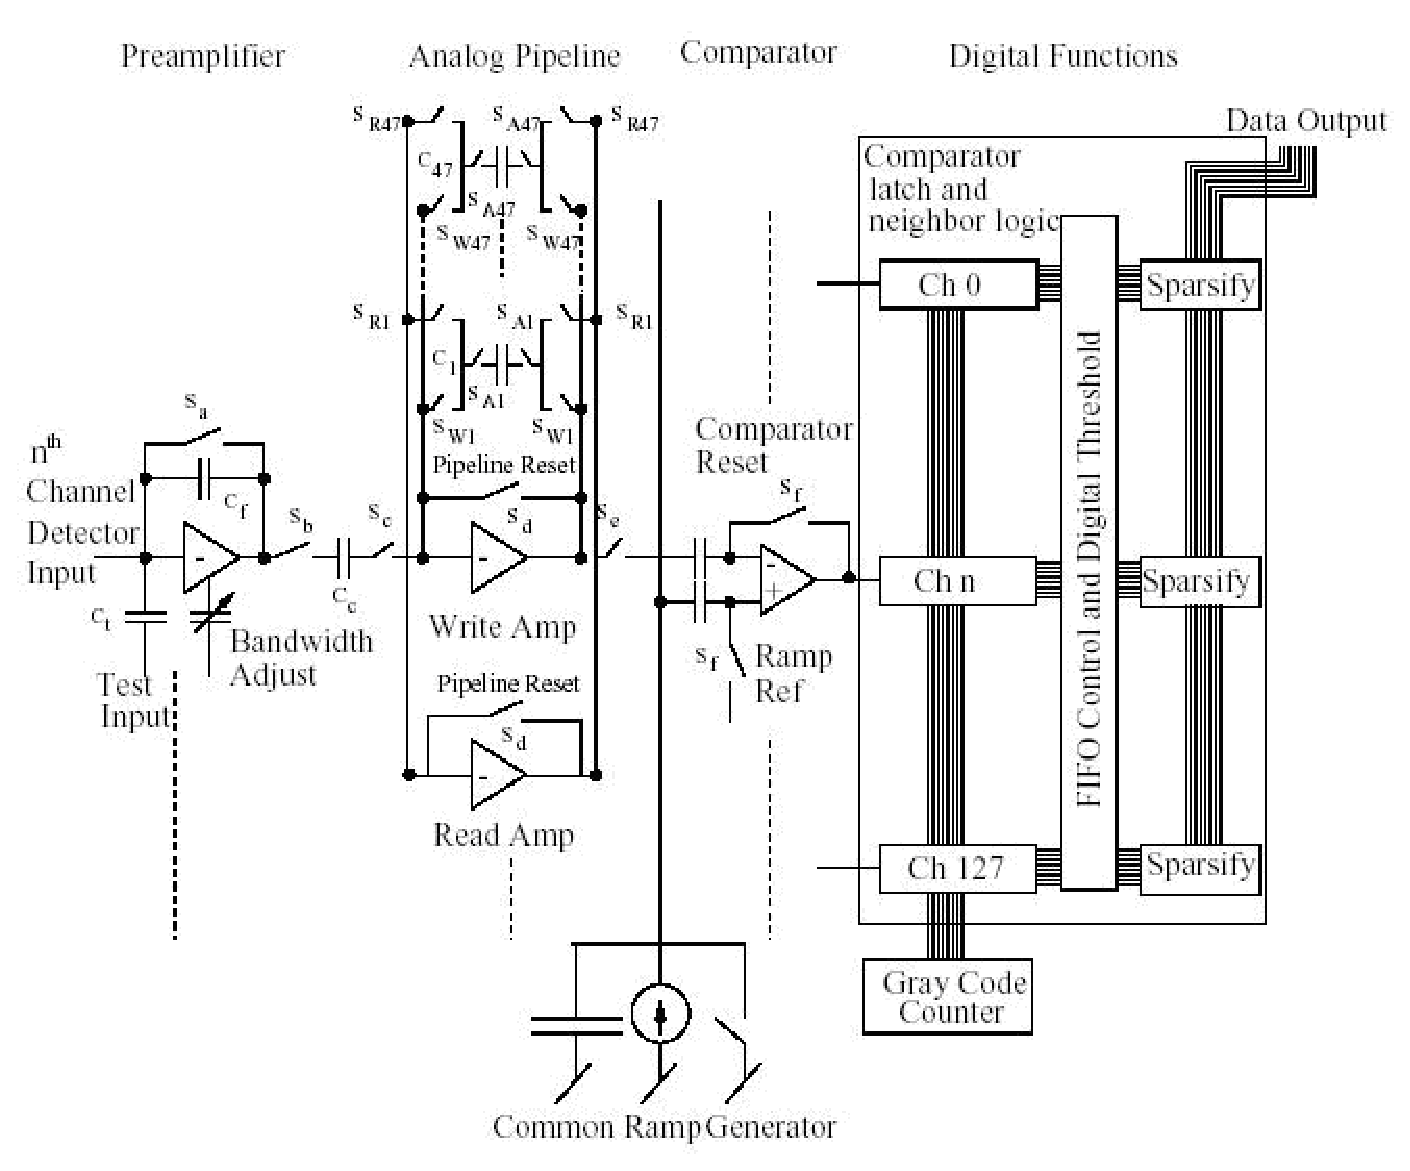
\includegraphics[width=0.75\textwidth]{svx-block}
\caption{\small{Block diagram of the SVX4.}}
\label{fig:svx-block}
\end{figure}
%%%%%%%%%%%%%%%%%%%%%%%%%%%%%%%%%%%%%%%%%%%%%%%%%%%%%%%%%%%%%%%%%%%%%%%

The Level-1 accept (L1A) signal to the ASIC is used to remove a ``hit'' 
cell from the pipeline.  The hit is temporarily stored in a FIFO buffer 
that can store up to four cells, corresponding to four L1As.  These hits 
are queued for readout to the back-end.  Once four cells are stored in 
the FIFO, additional L1As are ignored.  The trigger latency is programmed 
in the shift register during the initialize mode so that the right pipeline 
cell is read out.  L1A is normally high during acquisition and pulsed low 
to store a cell.  L1A must go low and return high between front-end clocks.  

The pedestal pipeline cell is reserved for acquiring only pedestal data.  
This cell is used during readout along with a stored cell.  The back-end 
digitizes the difference between the hit cell and the pedestal cell.  The 
pedestal cell is not part of the round robin ensemble of acquisition cells, 
hence the pedestal cell must be refreshed periodically.  Because of the 
continuous electron beam, L1A arrivals are not synchronized to the 
front-end clock, which implies that the associated detector signals are 
Poisson-distributed with respect to this clock.

SVX4 data acquisition rates at a luminosity of 
$1\times10^{35}$~cm$^{-2}$s$^{-1}$ were simulated to check their performance 
in a continuous electron beam environment.  The first aspect of the SVX4 
that was simulated was the L1A acceptance rate~\cite{CN2006-13}.  The 
triggers generated were Poisson-distributed with respect to the SVX4s FEClk.  
The simulation estimated the number of triggers that had an early arrival 
time and also estimated the number of triggers that were missed.  The results 
of the simulation showed that for half-field operation of the solenoid, 2.5~T, 
with an L1A rate of 10~kHz, $\sim$0.1\% of the triggers arrived early.  No 
triggers were missed.  The simulation was run for an L1A rate of 100~kHz as 
well, over ten times the expected trigger rate.  For these conditions only 
$\sim$1.3\% of the triggers arrived early and $\sim$0.3\% triggers were 
missed.

Another simulation checked the effect of issuing a reset and the associated 
restore operation when the pre-amplifiers on the chip saturate
\cite{CN2006-24}.  In operating the SVX4, charge is accumulated on the 
pre-amplifier and this charge needs to be periodically reset when it reaches 
$\sim$200~fC.  The results of these simulations show that at half-field of
the solenoid, a $\sim$1\% deadtime can be expected; at full-field operation 
the deadtime is $\sim$0.4\%.

SVX4 is designed for daisy-chained operation.  Daisy-chaining minimizes 
the number of bus and control lines required to operate the device.  Fewer 
control lines means less space on the high density interconnect and less 
mass in the system.  All the chips share a common communication bus and a 
common differential and back-end clock.  Each chip has two pads that are 
used for communication between adjoining chips.  After powering up the SVX4, 
the chip parameters must be downloaded before operation of the readout chips 
can begin.  For each SVX4 chip, 198 bits must be downloaded into the 
internal registers.

%%%%%%%%%%%%%%%%%%%%%%%%%%%%%%%%%%%%%%%%%%%%%%%%%%%%%%%%%%%%%%%%%%%%%%%
\begin{figure}[htbp]
\centering
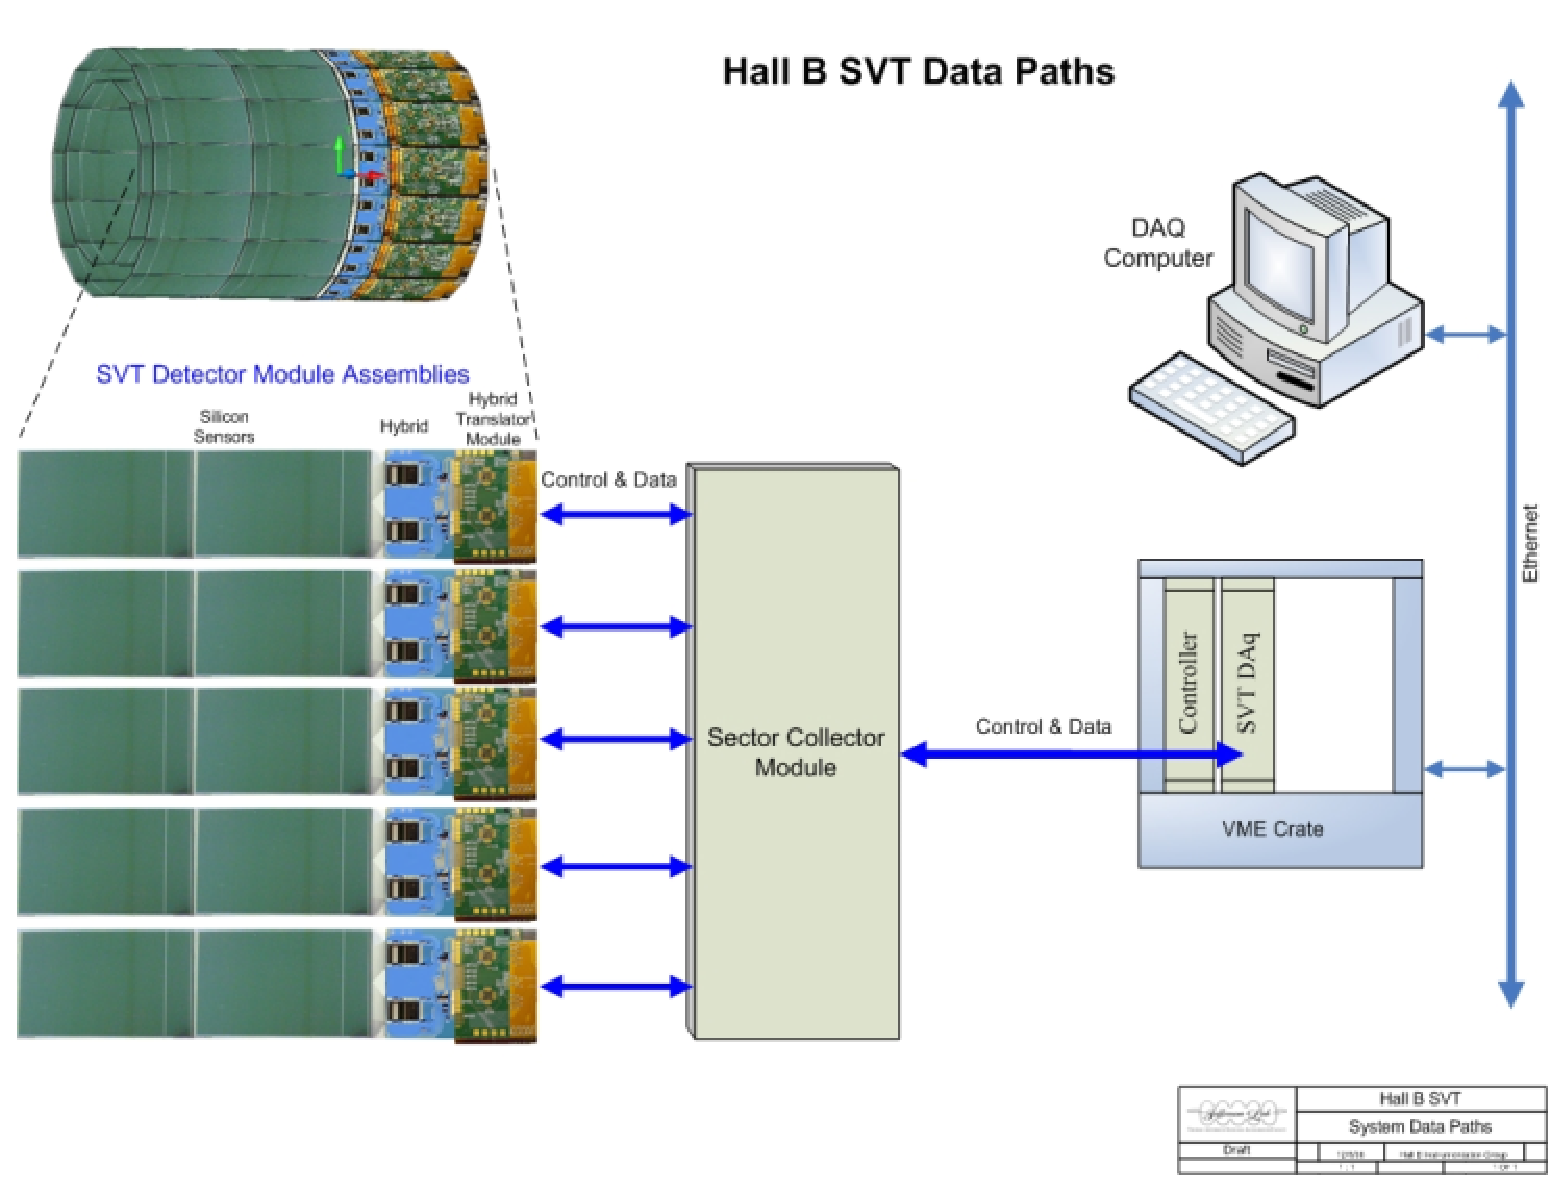
\includegraphics[width=0.70\textwidth]{data-path}
\caption{\small{SVT system data paths.}}
\label{fig:data-path}
\end{figure}
%%%%%%%%%%%%%%%%%%%%%%%%%%%%%%%%%%%%%%%%%%%%%%%%%%%%%%%%%%%%%%%%%%%%%%%

Fig.~\ref{fig:data-path} shows the data path for the Hall B SVT system.
Signals are digitized in the SVX4 ASICs on the hybrids.  The control 
signals and data bus for a module are connected to a sector collector
module (SCM).  Up to five modules are connected to an SCM that buffers 
and passes the data and control signals to the DAQ system.  SCMs may also 
be daisy-chained together to form a longer readout chain.  The readout 
chain requires only one detector module buffered by a single SCM to form 
a valid control and data path.  Unused SCM inputs are bypassed.  Increasing 
the number of SCMs connected together increases the daisy-chain length and 
the DAQ readout time.  The fastest readout is accomplished by a single 
silicon detector module, SCM, and SVT DAQ module chain.  
Fig.~\ref{fig:scm-daisy-chain} shows the daisy chain connections through 
an SCM.

%%%%%%%%%%%%%%%%%%%%%%%%%%%%%%%%%%%%%%%%%%%%%%%%%%%%%%%%%%%%%%%%%%%%%%%
\begin{figure}[htbp]
\centering
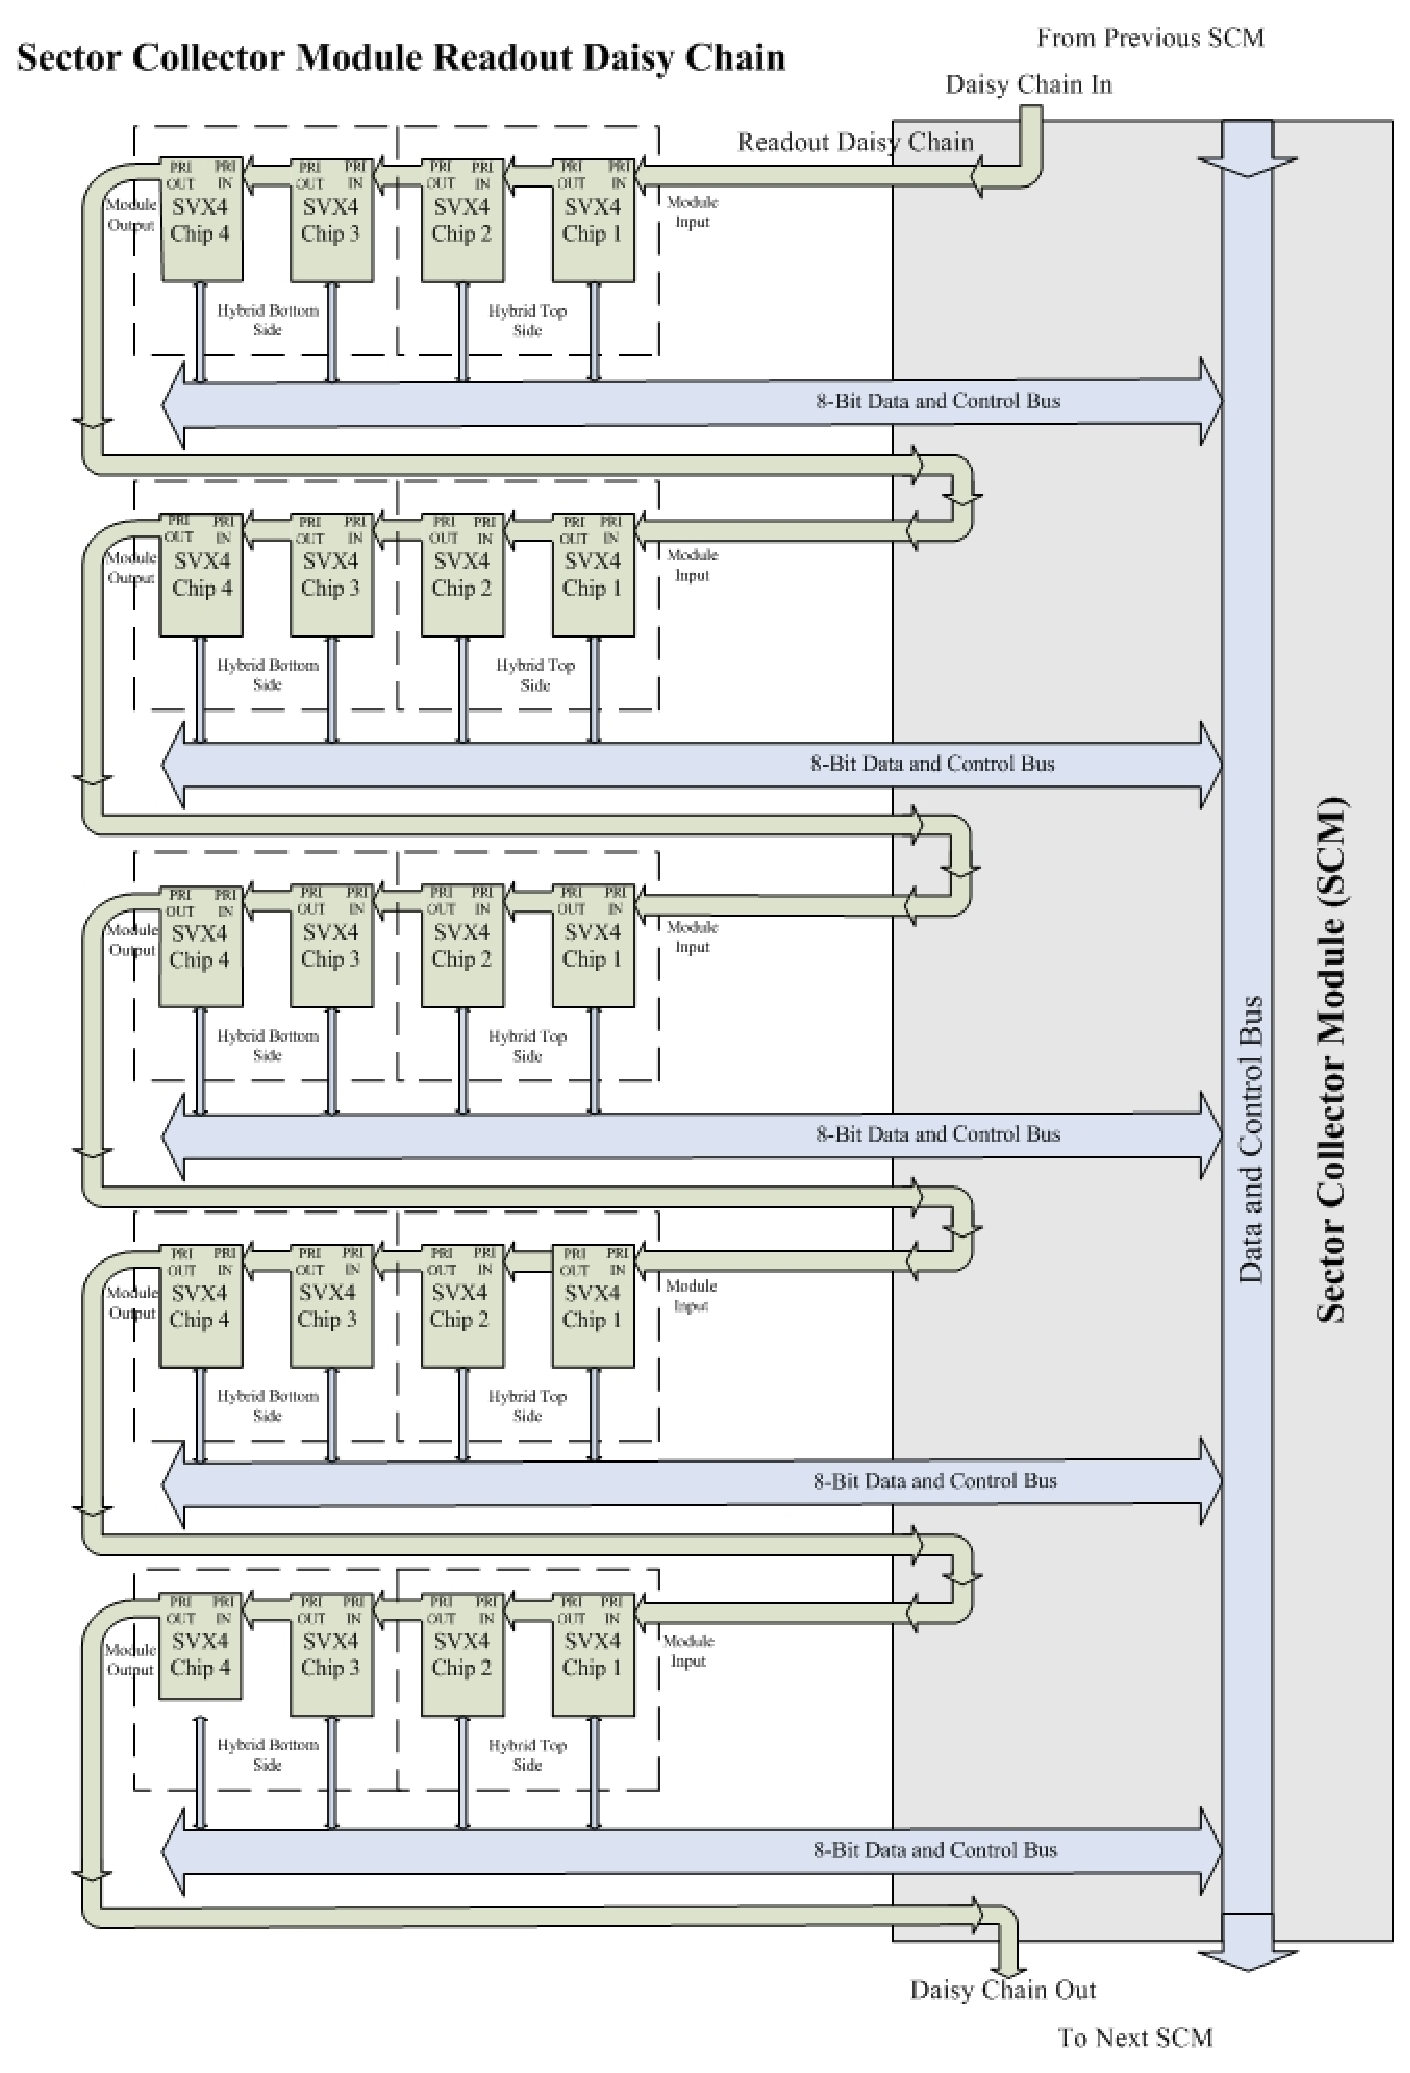
\includegraphics[width=0.6\textwidth]{scm-daisy-chain}
\caption{\small{Sector collector module daisy-chain readout.}}
\label{fig:scm-daisy-chain}
\end{figure}
%%%%%%%%%%%%%%%%%%%%%%%%%%%%%%%%%%%%%%%%%%%%%%%%%%%%%%%%%%%%%%%%%%%%%%%

For the {\tt CLAS} upgrade, VME systems will be used for both DAQ and slow 
controls.  Currently, {\tt CLAS} uses about 30 VME crates and several types 
of modules.  As a standard DAQ framework at JLab, 6U VME single board 
computers (SBCs) running VxWorks RTOS are used.  The Harvard-designed 
Silicon Readout Controller (SRC) used in FNAL-CDF was studied for possible 
implementation in our system.  This controller was originally designed for 
SVX3 readout.  The CDF-SRC printed circuit board is in 9U VME format.  This 
format is incompatible with our 6U-sized systems.  The board has nine FPGAs 
and only controls the SVX3 ASIC.  Separate VME hardware is needed to handle 
and store the data received from the silicon sensors.  In addition, this 
SRC is application specific for the pulsed accelerator at FNAL and designed 
around the triggering system used at CDF.

For control and data acquisition for the SVT, a 6U VME board compatible 
with the {\tt CLAS} data stream format is being developed~\cite{CN2004-04}.
This modular SRC will control and integrate the data received from the SVT 
readout chain into the DAQ system.  Fig.~\ref{fig:src-block} shows the block 
diagram of the prototype SRC.  The heart of the SRC design is 
Field-Programmable Gate Arrays (FPGAs).  The advantage of FPGA technology 
is that it combines the ease of software with the speed of hardware with 
permanent upgrade capabilities via downloaded updates.  FPGAs have already 
provided the lab with versatile VME bus data acquisition and control 
interfaces.  Current JLab FPGA designs provide control and monitoring for 
numerous systems by interfacing sensors and instrumentation with ADCs and
TDCs.  As shown in Fig.~\ref{fig:src-block}, data and control signals from 
the readout chain connect to the SVX4 controller FPGA logic for processing.  
Interface I/O signals are provided by the FPGA for external triggering, 
clock, and phase lock interfaces among others.  The FPGA has a memory 
management unit and PCI interface that connects to the VME interface.  
On-board memory stores the events to be read out.  The VME slave interface 
completes the data and control path to the VME backplane through bus 
transceivers.

%%%%%%%%%%%%%%%%%%%%%%%%%%%%%%%%%%%%%%%%%%%%%%%%%%%%%%%%%%%%%%%%%%%%%%%
\begin{figure}[htbp]
\centering
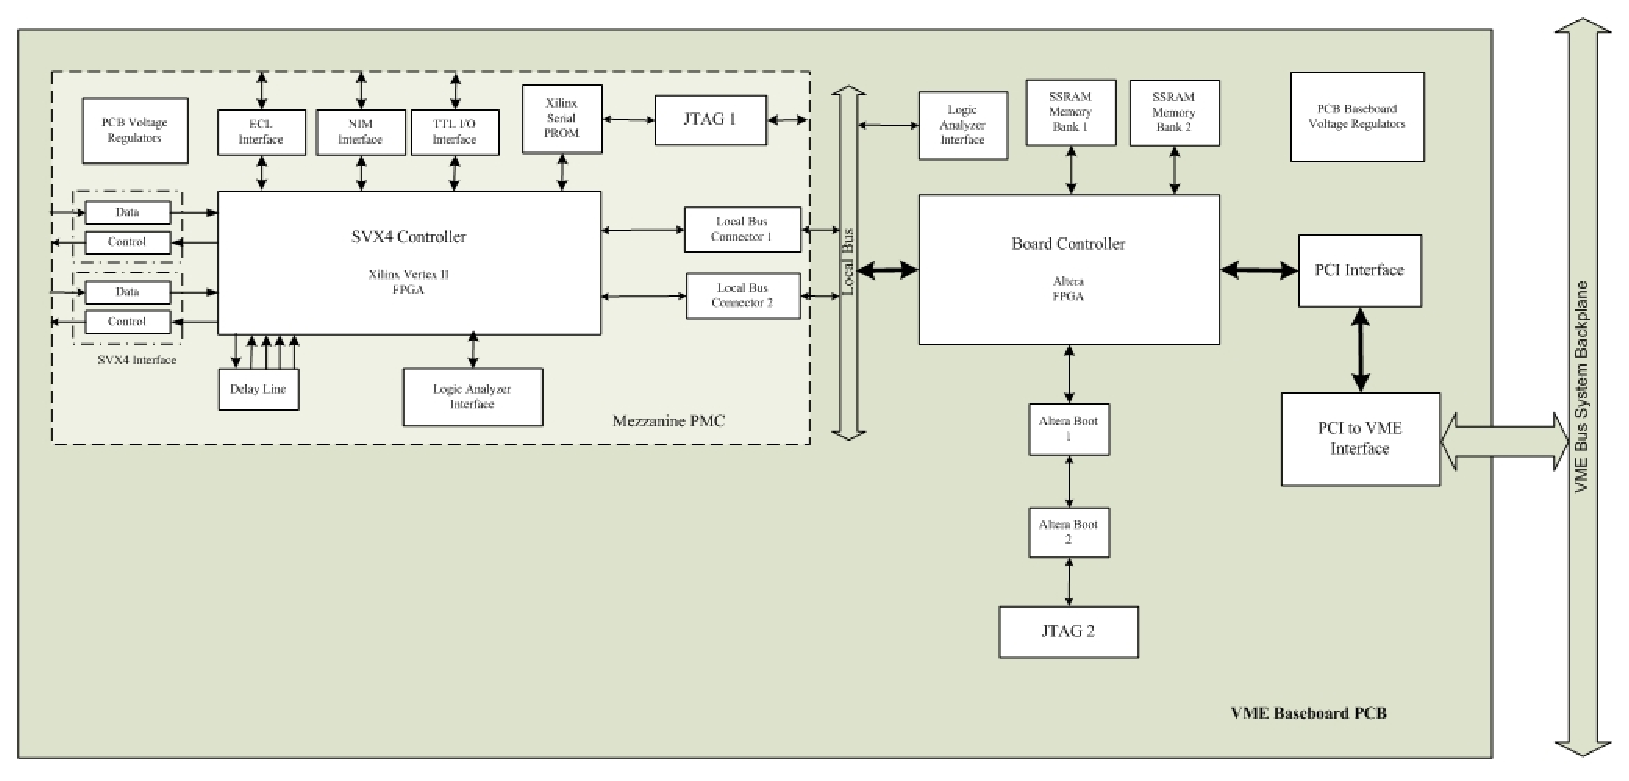
\includegraphics[width=0.7\textwidth]{src-block}
\caption{\small{SRC prototype block diagram.}}
\label{fig:src-block}
\end{figure}
%%%%%%%%%%%%%%%%%%%%%%%%%%%%%%%%%%%%%%%%%%%%%%%%%%%%%%%%%%%%%%%%%%%%%%%

The SRC generates initialize, acquisition, digitization, and readout 
timing sequences for the SVX4 ASIC.  The initialization cycle is typically 
performed once, followed by repetitive data acquisition, digitization, and 
readout sequences.  Since we will be operating the SVX4 ASIC in 
continuous data format mode, the acquisition cycle occurs simultaneously 
with the digitize and readout sequences.  After the hit cell has been 
digitized in the SVX4, the SRC starts a readout cycle and the event data 
is stored locally.  The event data will be continuously stored until the 
SRC is instructed to read out the data by the VME system controller or 
until the local memory is full.  The VME slave interface on the SRC accepts 
instructions from the VME SBC.  These instructions control the SVX4 
sequences and read out the stored events.  The SRC status register reports 
on the operating condition of the board including memory overflow.

The SRC design includes a Joint Test Action Group (JTAG) interface that 
provides In System Programming (ISP) capability.  The ability to reprogram 
the on-board components provides a permanent upgrade path via software 
updates.  It also provides a way to implement new features (even remotely) 
into an existing system after fabrication and installation.  In addition, 
JTAG technology can be used for board level interconnection and 
functionality testing.

Based on the GEANT3 simulation, approximately 16 particles will be 
generated per trigger in the cone part of the SVT when the solenoid is 
operating at half-field.  The forward cone is split into four groups, 
three of which have six modules and the last group has four modules.  The 
four group partition results in four tracks per group per trigger.  Six 
modules have 24 ASICs in all.  For each chip, the pipeline cell and ID has 
to be read; this contributes 96 bytes, whether or not there is data.  Four 
tracks in a group give rise to 6 hits, each of which requires a byte for 
cell ID and a byte for content, contributing 12 bytes per track.  Therefore 
there are 48 bytes per track from hits alone.  Therefore, there are 144 
bytes per trigger.  Since the groups are independently read out, this data 
rate translates to 1.44~MB/s for a trigger rate of 10~kHz, well below the 
56~MB/s readout rate capable by the ASIC.  Our expectations for the time 
taken for digitization and readout as a function of the number of hits in 
a sector of the FST have been computed and are shown in Fig.~\ref{readtiming}.
Each sector can handle up to 2500 hits in 105~ns (25~MHz).  A higher rate 
implies that before the digitization process can be completed a new L1A 
arrives, eventually filling up the FIFO and leading to a loss of triggers.

%%%%%%%%%%%%%%%%%%%%%%%%%%%%%%%%%%%%%%%%%%%%%%%%%%%%%%%%%%%%%%%%%%%%%%%
\begin{figure}[htbp]
\centering
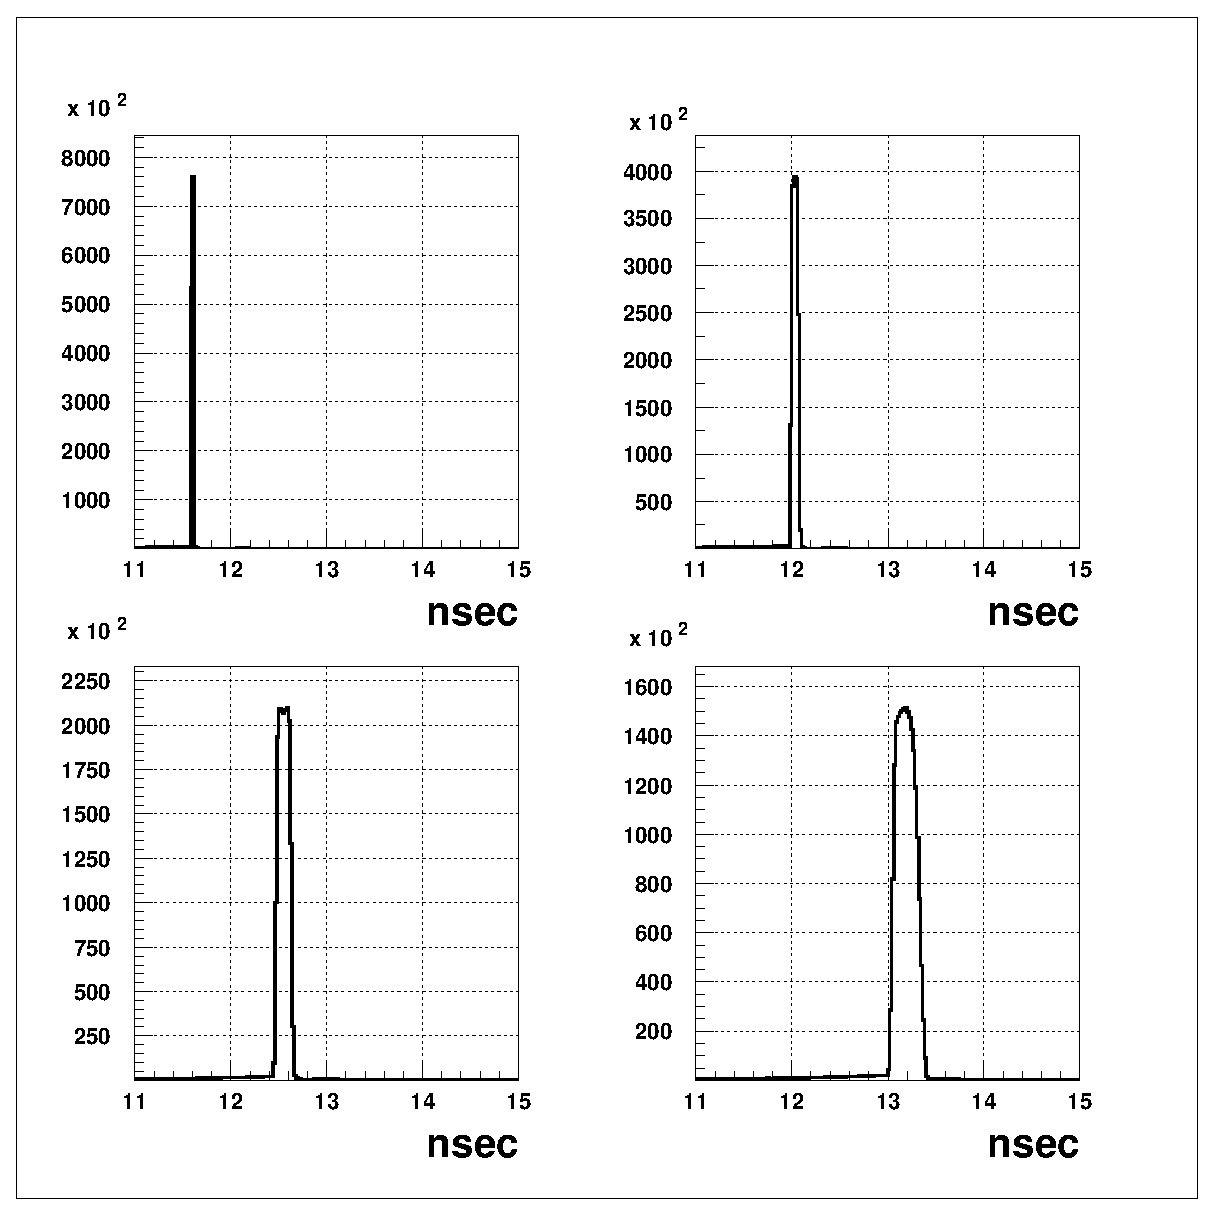
\includegraphics[width=0.8\textwidth]{timing}
\caption{\small{Readout time as a function of the number of hits in a
given layer or portion of the SVT.}}
\label{readtiming}
\end{figure}
%%%%%%%%%%%%%%%%%%%%%%%%%%%%%%%%%%%%%%%%%%%%%%%%%%%%%%%%%%%%%%%%%%%%%%%

\section{Research \& Development}

R\&D for the SVT system started in FY2004~\cite{CN2004-29}.  The R\&D 
goals are to evaluate silicon strip detector systems, assess compatibility 
of SVX4 performance with {\tt CLAS12} requirements, study the features of 
the FNAL stave design that could be useful for {\tt CLAS12}, and gain 
experience and know-how about developing support fixtures, installation, 
and DAQ by conducting lab tests and installing a test stave in Hall B for
in-beam tests~\cite{CN2004-42}.  

The initial R\&D effort~\cite{CN2005-009,CN2005-016} focused on the DAQ 
system of the stave received from FNAL.  The Hall B Instrumentation 
Group modified the DAQ hardware and software to run lab and beam tests.  
Some of the significant modifications that were made were the addition of 
plots to show the number of hits in each strip, the archiving of selected 
real-time strip plots, the storage of output data for off-line analysis, 
the ability to change the clock-base, and the addition of the external 
trigger mode.  For the operation of the stave, low and high voltage control 
programs were researched, developed, and implemented
\cite{CN2005-017,CN2005-018}.  

R\&D activities during FY2004 culminated with the conduction of beam tests
\cite{CN2005-020}.  To perform these tests, specialty cables, data 
buffers, data repeaters, controls and monitoring programs for low and high 
voltages, DAQ software, off-line analysis software, support structures, and 
finite element analyses were designed, developed, debugged, and implemented.  
The significant result of the FY2004 R\&D effort was that it provided 
hands-on experience with several facets of the endeavor to build a reliable 
state-of-the-art silicon vertex tracker tailored to meet {\tt CLAS12} 
requirements.  For FY2005 the R\&D plan was to develop a laser test stand 
and a PCI-based DAQ board~\cite{CN2005-019}.  However, due to budgetary 
considerations, work was done only on the laser test stand.  Additionally,
the prototype FPGA-based, PCI-bus-compatible, printed circuit carrier board 
for the DAQ controller of the SVT was successfully built and tested
\cite{CN2006-010} (see Fig.~\ref{fig:marc1}). 

%%%%%%%%%%%%%%%%%%%%%%%%%%%%%%%%%%%%%%%%%%%%%%%%%%%%%%%%%%%%%%%%%%%%%%%
\begin{figure}[htbp]
\centering
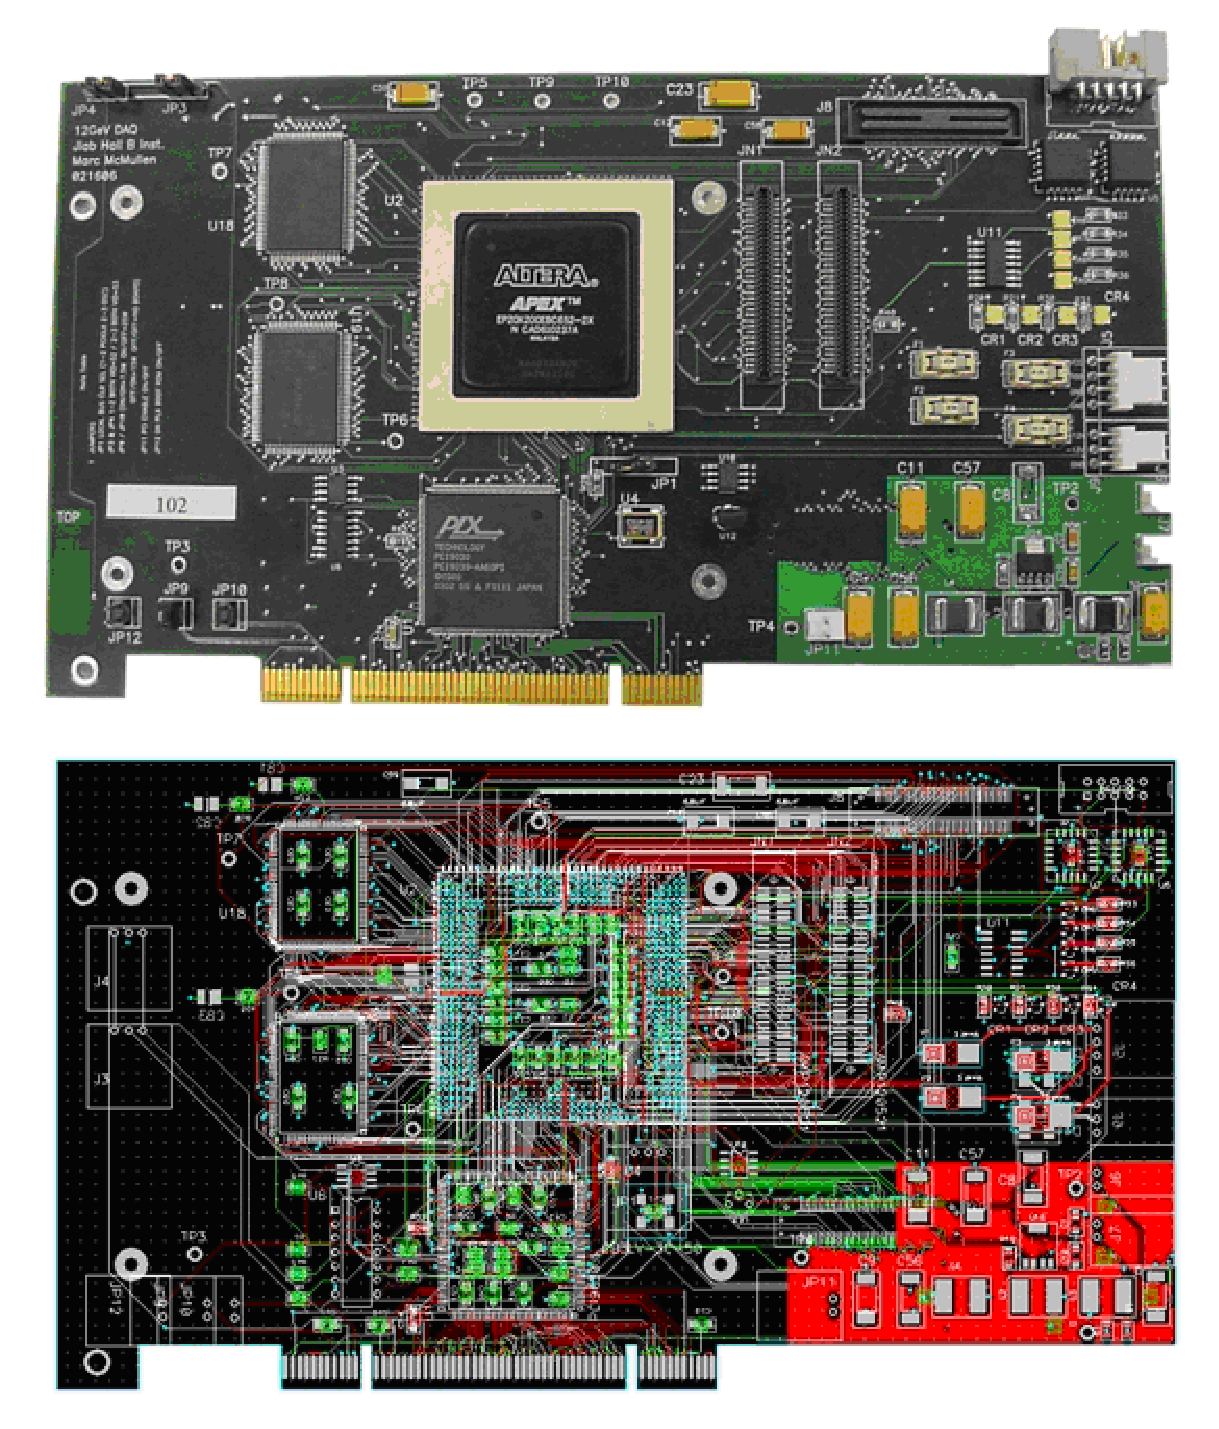
\includegraphics[width=0.45\textwidth]{marc1}
\caption{\small{New PCI-based {\tt CLAS12} DAQ base board.}}
\label{fig:marc1}
\end{figure}
%%%%%%%%%%%%%%%%%%%%%%%%%%%%%%%%%%%%%%%%%%%%%%%%%%%%%%%%%%%%%%%%%%%%%%%

%%%%%%%%%%%%%%%%%%%%%%%%%%%%%%%%%%%%%%%%%%%%%%%%%%%%%%%%%%%%%%%%%%%%%%%
\begin{figure}[htbp]
\centering
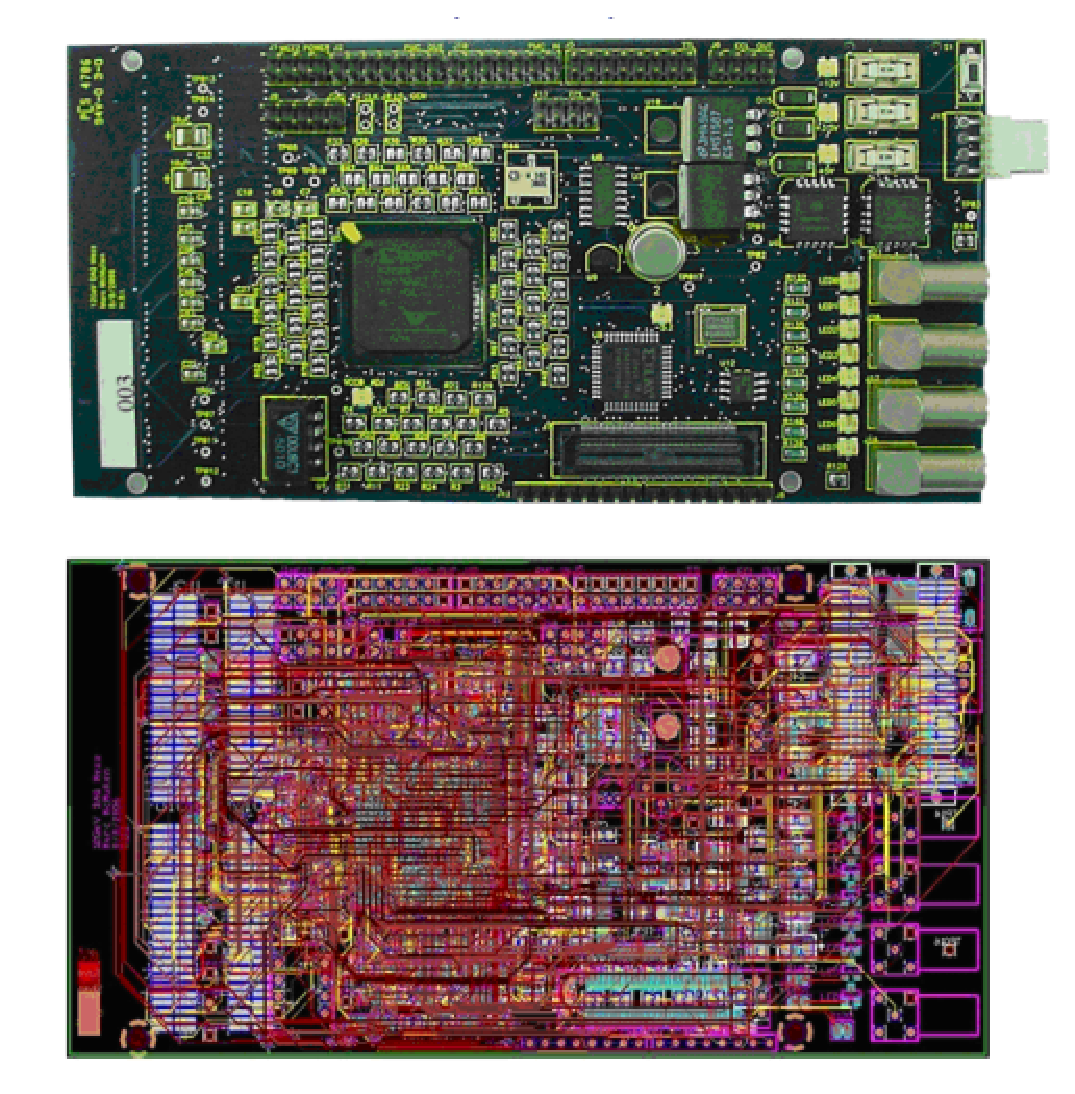
\includegraphics[width=0.5\textwidth]{marc2}
\caption{\small{SVX4-based PMC controller card.}}
\label{fig:marc2}
\end{figure}
%%%%%%%%%%%%%%%%%%%%%%%%%%%%%%%%%%%%%%%%%%%%%%%%%%%%%%%%%%%%%%%%%%%%%%%

R\&D for FY2006 focused on the design of the DAQ mezzanine circuit board
(shown in Fig.~\ref{fig:marc2}) that will be compatible with a VME board.  
The block diagram for the circuit board is shown in 
Fig.~\ref{fig:daq-pcb-block}.  The FPGA design of the SVT DAQ/controller 
board is flexible and permits use of different silicon sensor readout ASICs.

%%%%%%%%%%%%%%%%%%%%%%%%%%%%%%%%%%%%%%%%%%%%%%%%%%%%%%%%%%%%%%%%%%%%%%%
\begin{figure}[htbp]
\centering
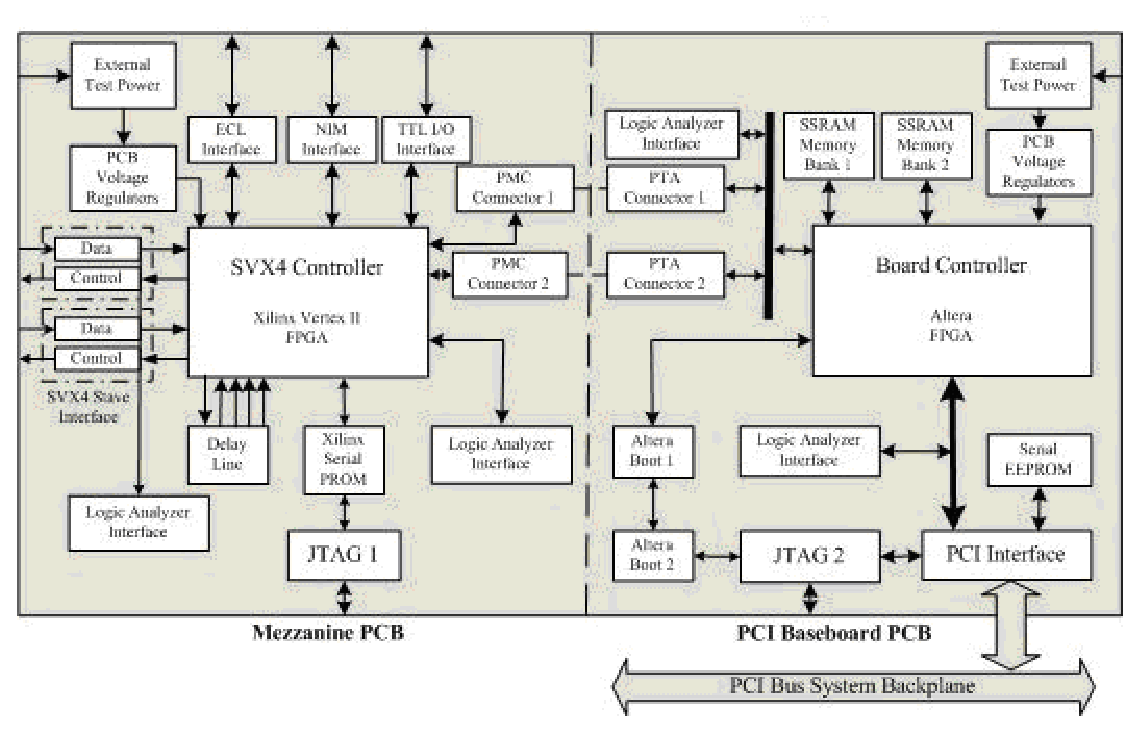
\includegraphics[width=0.75\textwidth]{daq-pcb-block}
\caption{\small{Prototype DAQ circuit board diagram.}}
\label{fig:daq-pcb-block}
\end{figure}
%%%%%%%%%%%%%%%%%%%%%%%%%%%%%%%%%%%%%%%%%%%%%%%%%%%%%%%%%%%%%%%%%%%%%%%

R\&D on the advanced conceptual design for the SVT is continuing.  Support 
structures and instrumentation strategies are being developed, and detector 
installation procedures are being studied.  Safety issues for each step of 
the detector construction and installation are being analyzed.

\section{SVT Commissioning and Operation}

The objective of the SVT commissioning plan is to debug, fix, and
calibrate system components.  Over the last several decades, much
experience in this area has been gathered by experiments at other
facilities.  The SVT commissioning program will draw on these experiences.
The commissioning plan includes studies without and with beam.

After installation of the SVT in the solenoid, a complete set of system
checks will be performed.  First, a visual inspection of cables and
electronics will be carried out.  Control, data, low voltage (LV), high
voltage (HV), and monitoring cables will be checked for proper strain relief,
sheathing, insulation integrity, and connections.

The detector will be monitored continuously by the {\tt CLAS12} slow controls
system.  The slow controls procedures to adjust critical parameters of the
equipment will be checked.  Power will not be turned on until all alarms and
fail-safe systems have been verified.  Power-up tests will be conducted first
on dummy loads.  This checkout will include all systems controlled by EPICS
as well.

Temperature and humidity conditions in and around the SVT will be monitored
continuously.  Also, light sensors inside the SVT will monitor the level of
light infiltration.

The LV system, including LV distributions, will be checked with dummy loads.
Correlations between demand, monitored, and measured voltages will be logged.
Once it is ascertained that the LV system is functional, it will be connected
to the SVT.  The HV system will be checked in a similar fashion.

Once both the LV and HV systems have been checked, the SVT will be powered
up; the power-up sequence will be, first the LV system, and then the HV
system.  The powering up of both the systems will be done in appropriate steps.
Current draw by both the systems will be automatically recorded.

Read/write tests on the ASIC registers will check whether all ASICs are able
to be programmed and whether they can be read back.  Calibration of the detector 
modules and testing of the readout chain will be accomplished by inputting an 
external signal.  This external input on each SVX4 ASIC has the capability of
injecting a small charge via a small charge injection capacitor (25~fF).  
Calibration will be done with different inject masks.  The acquired ADC spectra
will be used to calibrate the ASICs.  The performance of the system, including 
that of the front-end electronics, will be checked at the channel level by 
inspecting the occupancy plots.

Hit/no hit data will indicate noisy or dead channels.  An effort will be
made to fix channels with problems by appropriate measures, such as varying
the threshold, low, and high voltage values.

Once these basic tests have been completed, efficiency and tracking accuracy
tests will be performed using cosmic rays.  Cosmic triggers generated by the
CTOF will be used to measure the efficiency and the track reconstruction
accuracy in the Barrel Silicon Tracker.  These tests will be done for zero,
half, and full fields of the solenoid.  Tracks will be reconstructed in the
eight SVT layers in the upper hemisphere and the projected track hits will
be checked against the registered hits in the eight layers of the opposite
hemisphere.  These tests will be repeated with test beam.

\section{{\tt CLAS12} Drift Chambers}

\subsection{Overview}

The overall tracking requirements (0.5 -  1\% fractional momentum resolution 
at 5~GeV and efficient tracking at a luminosity of 
10$^{35}$~cm$^{-2}$s$^{-1}$) are the main drivers for drift chamber design.  
Because the {\tt CLAS} drift chamber system~\cite{dcnim} has operated 
successfully for 8~years, we plan to re-use many of the design concepts and 
most of the utility infrastructure.  In particular, we plan to re-use the 
present gas mixing and handling system, the high-voltage and low-voltage 
systems, the FASTBUS TDC system, and the post-amplifier/multiplexer systems.
The construction project thus consists of new chambers, on-board electronics, 
and on-board jumper cables.

The forward tracking system consists of three regions divided into six
sectors as shown in Fig.~\ref{umbrella}; located just before, inside, 
and just outside the torus field volume, and referred to as Regions~1, 2, 
and 3.  Each chamber will have its wires arranged in two superlayers of
six layers each, with the wires in the two superlayers strung with 
$\pm$6$^\circ$ stereo angles, respectively.  The cell structure will be 
hexagonal, that is, each sense wire is surrounded by six field wires.  This 
arrangement is similar to the present {\tt CLAS} design and offers good 
resolution with very good pattern recognition properties.  Refer to our 
article on the overall {\tt CLAS} detector~\cite{clasnim} and our article 
on the drift chambers themselves~\cite{dcnim} for details of the present 
detector and chambers.  The groups responsible for the {\tt CLAS12} drift
chamber construction include Old Dominion University, Idaho State
University, and Jefferson Laboratory.

%%%%%%%%%%%%%%%%%%%%%%%%%%%%%%%%%%%%%%%%%%%%%%%%%%%%%%%%%%%%%%%%%%%%%%%%
\begin{figure}[htbp]
\vspace{10.6cm}
\special{psfile=umbrella.ps hscale=60 vscale=60 hoffset=60 voffset=0}
\caption{\small{Schematic layout of the {\tt CLAS12} Forward Drift Chambers: 
Regions~1, 2, and 3.}}
\label{umbrella}
\end{figure}
%%%%%%%%%%%%%%%%%%%%%%%%%%%%%%%%%%%%%%%%%%%%%%%%%%%%%%%%%%%%%%%%%%%%%%%%

The major difference in the drift chambers for {\tt CLAS12} is that the 
cells cover a smaller solid angle than those in the present {\tt CLAS} 
chambers, allowing efficient tracking at higher luminosities because the 
accidental occupancy from particles not associated with the event is smaller.  
Table~\ref{fwd-dc-design-parms} lists the main design parameters for each 
region of the {\tt CLAS12} drift chambers.  For the purposes of simulating 
track resolutions, we assumed that the position resolution of the individual 
drift cells would be 250~$\mu$m.  

%%%%%%%%%%%%%%%%%%%%%%%%%%%%%%%%%%%%%%%%%%%%%%%%%%%%%%%%%%%%%%%%%%%%%%%%%
\begin{table}[ht]
\begin{center}
\begin{tabular} {||c|c|c|c||} \hline \hline
                     &{\bf Region 1}&{\bf Region 2}&{\bf Region 3}\\ \hline
Distance from target & 2.3 m    & 3.5 m        & 4.7 m    \\ \hline
Num. of superlayers  & 2        & 2            & 2        \\ \hline
Layers/superlayer    & 6        & 6            & 6        \\ \hline
Wires/layer          & 112      & 112          & 112      \\ \hline
Cell size            & 0.75 cm  & 1.18 cm      & 2.07 cm  \\ \hline
Active time window   & 150 ns   & 250 - 500 ns & 500 ns   \\ \hline
Resolution per wire  & 0.020 cm & 0.025 cm     & 0.030 cm \\ \hline
\end{tabular}
\caption{\small{Design parameters for the {\tt CLAS12} drift chambers.}}
\label{fwd-dc-design-parms}
\end{center}
\end{table}
%%%%%%%%%%%%%%%%%%%%%%%%%%%%%%%%%%%%%%%%%%%%%%%%%%%%%%%%%%%%%%%%%%%%%%%%%

There are also other differences in the design of the {\tt CLAS12} chambers 
compared to the current {\tt CLAS} chambers.  ways.  Successive superlayers 
have their wires arranged with a $\pm$6$^\circ$ stereo angle; the present 
arrangement has an axial layer and a 6$^\circ$ stereo layer.  For the present 
{\tt CLAS} detector, the $\phi$ resolution times $\sin \theta$ is about two 
times larger than the $\theta$ resolution.  To have more equal resolution in 
the two angles, we doubled our stereo angle from 0 and 6$^\circ$ to 
$\pm$6$^\circ$.  Unlike the present chambers, all of the wires in one of the 
superlayers are strictly parallel, and in a plane perpendicular to the wire 
direction, form perfect hexagons.  This should allow a more accurate drift 
velocity calibration than the current design with its layer-to-layer increase 
in cell size.  The choice of gas; a 92:08 Argon:CO$_2$ mixture is a small 
departure from our present 90:10 mixture and should result in a higher and 
more constant drift velocity.  We plan to run with a gas gain of 
$5 \times 10^4$.

Another departure from the present design is to design every chamber (in 
all three regions) to be self-supporting in order to ensure that they are 
easy to install and remove for maintenance.  In the present {\tt CLAS}, the 
Region~1 chambers are all bound together into a single unit in order to 
maintain the wire tension without excessively thick endplates, and the 
Region~2 chambers are actually mounted onto the magnet cryostat, with the 
cryostat itself maintaining the internal wire tensions.  None of the present 
Region~1 or 2 chambers can be accessed individually without a lengthy 
``tension-transfer'' process.  To avoid this, we are designing the Region~1 
and Region~2 chambers to be self-supporting like our present Region~3 
chambers.  To keep a very thin endplate (to minimize dead area), some of the 
wire tension in the Region~2 chambers may be borne by springs mounted to the 
torus cryostat, but many fewer springs than in the present detector.  The 
key to these improvements will be ultra-stiff endplate assemblies that 
obtain their stiffness by a flanged design.  

A third design change is to use 30-$\mu$m diameter sense wire rather than 
the presently-used 20~$\mu$m wire.  Our choice of wire is 30-$\mu$m diameter, 
gold-plated tungsten for the sense wires, 140-$\mu$m diameter, gold-plated 
aluminum for the field wires, and 140-$\mu$m diameter, stainless steel for
the guard wires.   This should make the chamber more robust to wire 
breakages.  Higher voltages will be required to achieve the same gas gain, 
and the resulting higher electric field in the drift cells will result in 
a more nearly constant drift velocity that should be easier to calibrate.
Prototypes are being built to study possible negative side-effects of the 
higher voltage operation, such as leakage currents on the circuit boards 
and/or higher rates of cathode emission from the field wire surfaces.

Fig.~\ref{garfield} shows GARFIELD calculations for a Region~3 drift cell
with both a 20-$\mu$m and a 30-$\mu$m diameter sense wire.  Here the
cells with the thicker sense wire will have a significantly higher drift 
velocity, which is desirable to reduce the time window, and hence the 
chamber occupancy.

%%%%%%%%%%%%%%%%%%%%%%%%%%%%%%%%%%%%%%%%%%%%%%%%%%%%%%%%%%%%%%%%%%%%%%%%%%%
\begin{figure}[ht]
\vspace{12.0cm}
\special{psfile=garfield1.eps hscale=30 vscale=27 hoffset=40 voffset=165}
\special{psfile=garfield2.eps hscale=30 vscale=27 hoffset=40 voffset=-5}
\special{psfile=garfield3.eps hscale=30 vscale=27 hoffset=230 voffset=165}
\special{psfile=garfield4.eps hscale=30 vscale=27 hoffset=230 voffset=-5}
\caption{\small{GARFIELD calculations of the electric field lines (top)
and drift time vs. drift distance (bottom) for a Region~3 drift cell.  The 
left plots show the configuration with a 20-$\mu$m diameter sense wire and 
the right plots show the configuration with a 30-$\mu$m diameter sense wire.
The high voltages were set to provide the same gas gain for each
configuration.}}
\label{garfield}
\end{figure}
%%%%%%%%%%%%%%%%%%%%%%%%%%%%%%%%%%%%%%%%%%%%%%%%%%%%%%%%%%%%%%%%%%%%%%%%%%%
 
\subsection{Mechanical Design}

The chambers are designed to position the wires with an accuracy of 
100~$\mu$m and to be robust and easily serviceable.  The chambers are 
being designed with in-position surveying in mind.  In order to cover 
angles down to 5$^\circ$, the dead areas of each chamber (endplates, 
printed circuit boards, etc.) must be made as small as possible.  The 
chambers in the high-field region (Region~2) must not be susceptible to 
eddy-current forces that might arise in the event of a quench of the 
superconducting torus.

We have arrived at different solutions for the three regions, but they
share some characteristics:

\begin{itemize}
\item a very accurately drilled, flat endplate is affixed to a much stiffer
frame;
\item the flanges of the frame extend beyond the endplate thickness but
do not further increase the dead area of the chamber;
\item the chambers can be supported from two points only, at two ends of
the outer ``backplate'';
\item the Region~1 and Region~3 chambers are fully self-supporting in any 
orientation relative to gravity by the aforementioned two-point attachment;
\item to further minimize dead area, the Region~2 chambers may have a portion
of the wire tension borne by springs attached to the torus cryostats;
\item when out of position, the Region~2 chamber may have temporary posts
in compression taking the wire tension;
\item signal translator boards (STB) will be mounted on the chamber and
provide a connection between the wire crimp pins and the on-board 
preamplifier hybrid units;
\item similarly, on-board high-voltage translator boards (HVTB) provide a
connection to the high-voltage for each group of wires;
\item on-board cables will run from the STBs and HVTBs to a connector box 
on the backplate.
\end{itemize}

\subsubsection{Wire Layout: Cells, Layers, Superlayers}

The wires are laid out in a ``brick-wall'' pattern with a guard wire layer 
followed by two layers of field wires and one layer of sense wires in a 
repeating pattern.  Six layers of sense wires and their corresponding field 
and guard layers constitute a single superlayer.  All of the wires in one 
superlayer are parallel.  As we progress through the three regions, the 
superlayers are alternately $U$, $V$, $U$, $V$, $U$, $V$, with ``$U$'' 
representing wires with a +6$^\circ$ stereo angle and ``$V$'', -6$^\circ$.  
The present {\tt CLAS} detector has a similar wire layout structure and we 
have had very robust track-finding ability, even in the presence of modest 
backgrounds (up to 4\% occupancy levels).  Even in the presence of 
malfunctioning areas of the chambers, tracking is still efficient even with 
only 5 superlayers active.

The proposed chambers are planar; all wires in a given layer lie within
a plane, as opposed to the present {\tt CLAS} design where wires in a given 
layer lie on a cylindrical surface.  This has the advantage that all cells 
within a given layer are equal-sized, facilitating calibration.

%%%%%%%%%%%%%%%%%%%%%%%%%%%%%%%%%%%%%%%%%%%%%%%%%%%%%%%%%%%%%%%%%%%%%%%%%%%
\begin{figure}[htbp]
\vspace{9.0cm}
\special{psfile=dcassy.ps hscale=45 vscale=45 hoffset=100 voffset=-50}
\caption{\small{Assembly drawing showing the key elements of the drift
chamber box.  Gas window, electronic boards, and cables not shown.}}
\label{dcassy}
\end{figure}
%%%%%%%%%%%%%%%%%%%%%%%%%%%%%%%%%%%%%%%%%%%%%%%%%%%%%%%%%%%%%%%%%%%%%%%%%%%

\subsubsection{Endplates and Box Assembly}

The chamber body consists of a precisely drilled flat endplate fitted into 
a stiff, machined frame.  We have already completed the design of a 
full-sized Region~1 prototype chamber.  Fig.~\ref{dcassy} shows the 
essential elements of the drift chamber: the endplates, the ``backplate'', 
the stiffening ``rails'' into which the endplates fit, and the ``noseplate'' 
that fits into a common hexagonal support ring.  Fig.~\ref{endplate} shows 
design details for the endplate itself and Fig.~\ref{frame} shows how the 
endplates fit into the associated box frame.  Table~\ref{reg1-design-parms} 
lists the design parameters for the Region~1 prototype chamber.  
Fig.~\ref{reg1fea} shows expected deflections of the endplate assembly after 
stringing (relative to unstrung).

%%%%%%%%%%%%%%%%%%%%%%%%%%%%%%%%%%%%%%%%%%%%%%%%%%%%%%%%%%%%%%%%%%%%%%%%%%%
\begin{figure}[htbp]
\vspace{21.0cm}
\special{psfile=r1_proto_1.ps hscale=22 vscale=22 hoffset=-10 voffset=300}
\special{psfile=r1_proto_2.ps hscale=50 vscale=50 hoffset=80 voffset=0}
\caption{\small{Design drawings of a Region~1 endplate showing the dimensions,
hole locations, and tolerances.}}
\label{endplate}
\end{figure}
%%%%%%%%%%%%%%%%%%%%%%%%%%%%%%%%%%%%%%%%%%%%%%%%%%%%%%%%%%%%%%%%%%%%%%%%%%%

%%%%%%%%%%%%%%%%%%%%%%%%%%%%%%%%%%%%%%%%%%%%%%%%%%%%%%%%%%%%%%%%%%%%%%%%%%%
\begin{figure}[htbp]
\vspace{9.0cm}
\special{psfile=reg1_proto_exploded.ps hscale=45 vscale=45 hoffset=60 
voffset=260 angle=-90}
\caption{\small{Drawing to show how a Region~1 endplate fits into its 
associated frame.}}
\label{frame}
\end{figure}
%%%%%%%%%%%%%%%%%%%%%%%%%%%%%%%%%%%%%%%%%%%%%%%%%%%%%%%%%%%%%%%%%%%%%%%%%%%

%%%%%%%%%%%%%%%%%%%%%%%%%%%%%%%%%%%%%%%%%%%%%%%%%%%%%%%%%%%%%%%%%%%%%%%%%
\begin{table}[htbp]
\begin{center}
\begin{tabular} {||l|c||} \hline \hline
{\bf Parameter}              &  {\bf Value}      \\ \hline
Total weight                 & 160 kg            \\ \hline
Total wires                  & 4928              \\ \hline
Diameter,tension sense wires & 30 $\mu$m, 20 g   \\ \hline
Diameter,tension field wires & 140 $\mu$m, 63 g  \\ \hline
Diameter,tension guard wires & 140 $\mu$m, 285 g \\ \hline
Total wire tension           & 352 kg            \\ \hline
Endplate span                & 1.75 m            \\ \hline
Backplate span               & 1.75 m            \\ \hline
Max. endplate deflection     & 1.6 mm            \\ \hline
Max. gravitational wire sag  & 250 $\mu$m        \\ \hline \hline
\end{tabular}
\caption{\small{Design parameters for the single-sector Region~1 drift 
chamber prototype.}}
\label{reg1-design-parms}
\end{center}
\end{table}
%%%%%%%%%%%%%%%%%%%%%%%%%%%%%%%%%%%%%%%%%%%%%%%%%%%%%%%%%%%%%%%%%%%%%%%%%

%%%%%%%%%%%%%%%%%%%%%%%%%%%%%%%%%%%%%%%%%%%%%%%%%%%%%%%%%%%%%%%%%%%%%%%%%%%
\begin{figure}[htbp]
\vspace{8.5cm}
\special{psfile=r1_def.ps hscale=60 vscale=55 hoffset=40 voffset=0}
\caption{\small{Finite-element analysis of the Region~1 prototype endplate
showing expected deflections due to wire tension.  Note that the red
areas correspond to the maximum deflections of about 1.6~mm.}}
\label{reg1fea}
\end{figure}
%%%%%%%%%%%%%%%%%%%%%%%%%%%%%%%%%%%%%%%%%%%%%%%%%%%%%%%%%%%%%%%%%%%%%%%%%%%

\subsubsection{Wires, Feedthroughs, Crimp Pins}

Table~\ref{wirechoices} lists the materials and specifications for our wires, 
feedthroughs, and crimp pins.  Our endplates are not parallel to each other, 
but instead are oriented with respect to each other at an angle of 60$^\circ$.
For this reason, the wire position is fixed not by the location of the crimp, 
but by the position at which the wire leaves the end of the feedthrough.  This 
concept was tested before the present {\tt CLAS} construction.  The nominal 
wire-stringing tension was enough to force the wire to the ``bottom'' of the 
feedthrough mouth, establishing the position within an accuracy of 25~$\mu$m.  
Fig.~\ref{feedthrough} shows the details of a feedthrough penetration.

%%%%%%%%%%%%%%%%%%%%%%%%%%%%%%%%%%%%%%%%%%%%%%%%%%%%%%%%%%%%%%%%%%%%%%%%%
\begin{table}[htbp]
\begin{center}
\begin{tabular} {||c|c||} \hline \hline
{\bf Parameter}      &  {\bf Value} \\ \hline
end-plate material & Aluminum, Stesalit \\ \hline
frame material & stainless steel \\ \hline
gas-bag material & aluminized Mylar \\ \hline
sense wire material   & gold-plated tungsten \\ \hline
field wire material   & gold-plated aluminum \\ \hline
guard wire material   & stainless steel \\ \hline
feedthrough material & Noryl \\ \hline
crimp pin material & gold-plated copper (OFHC) \\ \hline \hline
\end{tabular}
\caption{\small{Material choices for the wires, feedthroughs, and crimp pins.}}
\label{wirechoices}
\end{center}
\end{table}
%%%%%%%%%%%%%%%%%%%%%%%%%%%%%%%%%%%%%%%%%%%%%%%%%%%%%%%%%%%%%%%%%%%%%%%%%

%%%%%%%%%%%%%%%%%%%%%%%%%%%%%%%%%%%%%%%%%%%%%%%%%%%%%%%%%%%%%%%%%%%%%%%%%%%
\begin{figure}[htbp]
\vspace{5.5cm}
\special{psfile=reg1_proto_wire_angle.ps hscale=55 vscale=55 hoffset=450 
voffset=-75 angle=90}
\caption{\small{Illustration of two neighboring endplates showing the 
feedthrough penetration on each and the wire strung between the two 
feedthroughs.}}
\label{feedthrough}
\end{figure}
%%%%%%%%%%%%%%%%%%%%%%%%%%%%%%%%%%%%%%%%%%%%%%%%%%%%%%%%%%%%%%%%%%%%%%%%%%%

\subsubsection{Attachment Points}

The chambers are being designed to be supported from two points on the 
backplate without imposing a large change of stress on the wires.  This will 
facilitate installation.  Fig.~\ref{dcassy} shows a sketch of the attachments 
on the backplate of the chamber.

\subsubsection{Survey, Alignment, and Magnetic Field Mapping}

The chambers are being designed with survey and alignment in mind.  For 
accurate tracking, the chamber locations must be well-known in space, 
especially with respect to the magnetic field.  Survey points will be 
located on accessible faces of the chamber frame.  Internal surveys 
(see Section~\ref{internal}) will transfer our knowledge of the location 
of the wire holes to these faces.

The magnetic field mapping strategy has not been worked out pending a final 
design of the torus magnet, but the concept will be to use hall probes to 
locate the positions of the energized conductors within the cryostats to 
sub-millimeter accuracy, and then to calculate the fields.  We will take 
advantage of the very precise magnetic probe technology now available, and 
also of sophisticated software packages to calculate fields.  This allows us 
to design small, precise instruments that can abut the cryostats themselves 
and be surveyed accurately.

\subsection{Electronic Readout}

The signal connections to the wires are made through printed-circuit 
boards mounted along one side of each chamber, called Signal Translator 
Boards (STBs).  These boards are responsible for signal routing and 
preamplification.  On the opposite side of each sector, another set of 
circuit boards called the High Voltage Translator Boards (HVTBs) is used 
to make the high-voltage connections to the wires.

\subsubsection{On-Chamber PCBs and Cables}

The {\tt CLAS12} wire chamber geometry changes significantly from {\tt CLAS}, 
so the circuit boards that interface the high voltages for the field, sense, 
and guard wires are new designs.  The circuit boards that interface the sense 
wires to the preamplifiers (STBs) are also new designs.   These interface 
circuit boards, both for the high voltage and the preamplifiers, will be 
designed on a 96-channel format.  This format will allow for only seven 
circuit boards for each superlayer.  Each sector in a particular region will 
use these seven circuit board formats for either high voltage or 
preamplification of the sense wire signal.  Table~\ref{electronic-channels} 
gives a channel count of the system.  Fig.~\ref{r1stb} shows the traces 
routed from the signal pick-up at the plated-through holes to the signal 
inputs of the preamplifier.

%%%%%%%%%%%%%%%%%%%%%%%%%%%%%%%%%%%%%%%%%%%%%%%%%%%%%%%%%%%%%%%%%%%%%%%%%%%
\begin{figure}[htbp]
\vspace{10.0cm}
\special{psfile=r1stb.ps hscale=80 vscale=80 hoffset=30 voffset=-40}
\caption{\small{Trace routing shown on one of the Region~1 STBs being
designed.}}
\label{r1stb}
\end{figure}
%%%%%%%%%%%%%%%%%%%%%%%%%%%%%%%%%%%%%%%%%%%%%%%%%%%%%%%%%%%%%%%%%%%%%%%%%%%

Fortunately the preamplifier used for the {\tt CLAS} drift chambers can 
still be manufactured and the components are readily available.  A large 
order for the {\tt CLAS} preamplifier, CP01, was ordered less than two 
years ago, as replacements for the original 1994 design.  The new order 
included an epoxy resin encapsulation of the components on the preamplifier 
single in-line package or SIP.  The encapsulation of the components on the 
hybrid SIP preamplifier is present to prevent component corrosion.

The CP01 preamplifier specifications are suitable for the {\tt CLAS12} wire 
chamber signal levels, and provide the gain, dynamic range, rise time, low 
noise, and low power for the upgrade performance requirements.  These 
preamplifiers were designed in unison with the Amplifier Discriminator 
Boards (ADBs), that provide another level of amplification and a monostable 
discriminator pulse with the threshold setting optimized for the best 
resolution or sensitivity to a minimum ionizing signal.  The monostable 
discriminated pulse widths are then multiplexed into a single channel of a 
pipeline TDC, with a least significant count of 500~ps and 8~$\mu$s of 
pipeline memory depth.

The low voltage power supplies used for {\tt CLAS} will be used for 
{\tt CLAS12}.  These units are robust and manufactured by Hewlett Packard.  
The supplies are remotely programmable and monitored, and will provide more 
than enough power for the new wire chamber preamplifier requirements.  We 
will use the same successful method of isolating the low voltage from 
ground loops, using local voltage regulators on the preamplifier interface 
boards (STBs).  The segmentation of the low voltage distribution cables is 
based on 32 preamplifier channels per supply cable.  Each of these supply 
cables is fused with an appropriate type of fuse rated for over-current 
protection based on 32 preamplifier loads.  We plan to re-use our CAEN 
system 527 high voltage supplies with somewhat finer segmentation than our 
current system, consistent with our total channel count dropping from 34000 
to about 24000.

We plan to use 17-pair twisted pair cable for routing our signals from the 
STBs to the chamber backplate.  The cable is round-jacketed with a 
0.025-in pitch so that the overall cable dimension is smaller than the 
standard 17-pair cable.  This smaller outer diameter cable will only be 
used from the STBs to the on-chamber ``service panels''.  The standard 
17-pair cable will be used from the chamber service panel to the readout 
electronics racks.

%%%%%%%%%%%%%%%%%%%%%%%%%%%%%%%%%%%%%%%%%%%%%%%%%%%%%%%%%%%%%%%%%%%%%%%%%
\begin{table}[htbp]
\begin{center}
\begin{tabular} {||c|c||} \hline \hline
{\bf Component}           & {\bf Number} \\ \hline
STB boards (6 types)      & 252 total \\ \hline
HVTB boards (6 types)     & 252 total \\ \hline
low-voltage cables        & 252 total  \\ \hline
high-voltage cables       & 252 total  \\ \hline
signal cables (17-pair)   & 1512 \\ \hline
total signals             & 24192 \\ \hline \hline
\end{tabular}
\caption{\small{Electronic channel counts for the readout, high voltage,
and low voltage.}}
\label{electronic-channels}
\end{center}
\end{table}
%%%%%%%%%%%%%%%%%%%%%%%%%%%%%%%%%%%%%%%%%%%%%%%%%%%%%%%%%%%%%%%%%%%%%%%%%

\subsubsection{Post-Amplifiers, Discriminators, Multiplexers, TDCs}

We plan to re-use our post-amplifier and discriminator boards, as well
as the associated multiplexing scheme.  We also plan to re-use our LeCroy 
1877 TDC modules.  For details of these systems, refer to our drift chamber 
technical paper in Ref.~\cite{dcnim}.

\subsection{Gas System}

We have an extensive gas-handling system that has performed well.  We plan 
to re-use it with only minor modifications of the plumbing.  Full details 
of this system and its design are described in our drift chamber technical 
paper in Ref.~\cite{dcnim}.

\subsection{Drift Chamber Construction}

The chambers are being designed with individual holes and holders for
each wire, i.e. a ``strung'' rather than a ``wound'' chamber.  Our 
inspection and assembly procedures are designed to produce devices with 
wires placed and known by external survey to an accuracy of 100~$\mu$m, 
in order to achieve our goal of a 250~$\mu$m positional accuracy per wire 
layer.  In addition to accuracy, we have chosen materials and designed 
procedures to insure a quiet and long-lived detector.  The construction 
and winding techniques are based on our already successful {\tt CLAS} 
drift chamber design.

\subsubsection{Inspection and Cleaning}

A visual and tactile inspection will be performed on the endplates and 
structural frame once we have accepted delivery.  If deemed necessary, 
the surfaces will be sanded using 320-grit paper on a orbital sander to 
de-burr them in preparation for measurements.  The endplates and structural 
frame will undergo a gross cleaning by soaking in a low residue laboratory 
degreasing solution with hand scrubbing, followed by a high-pressure water 
rinse. The parts will then receive their final cleaning using an ultrasonic 
bath of a laboratory-grade detergent solution.  After two hours they will 
be removed from the bath and rinsed with de-ionized water and then sprayed 
with methanol to aid drying. Once dry, the parts are heat-sealed in nylon 
bags with a nitrogen atmosphere to await assembly.

Smaller parts such as feedthroughs and hardware are cleaned using a 
bench-top ultrasonic cleaner with laboratory detergent, followed by a 
de-ionized water rinse and a dousing of methanol to facilitate drying.  
In addition, the injection-molded parts are specified to be free of silicon 
mold releases.

\subsubsection{Box Assembly}

The box assemblies for Regions~1 and 3 consist of a structural frame to 
which the endplates are attached.  This is achieved by first welding the 
frame to a reasonable tolerance then skim-cutting and drilling the 
endplate-receiving surfaces of the frame in a 5-axis milling machine.  The 
cleaned endplates and cleaned structural frame are then joined using pins 
to locate them with low out-gassing epoxy (Shell Epon 826 resin/Versamid 140 
hardener) on the contact surfaces and bolts to clamp and secure them.  When 
the epoxy has cured, the box assembly is sent to the measurement lab for 
fiducialization.  Once this is complete, the feedthroughs are inserted and 
set in place using the same epoxy that was used to bond the endplates to 
the frame.

\subsubsection{Internal Survey}
\label{internal}

A statistical sampling of the feedthrough hole locations and diameters 
will be performed on all endplates and structural components upon receipt 
from the vendor as part of the normal verification procedure.  The JLab
Survey Group will be using a Faro hard probe configuration on their portable 
coordinate measuring machine in a temperature-controlled laboratory for 
these measurements. The goal is to ensure the feedthrough holes are within 
the 0.200-mm true position tolerance and that the hole diameters are within 
the specified tolerance range. 

Once the box frame and endplates are assembled, and before the feedthroughs 
are installed, a seven parameter least squares transformation is used to 
fiducialize the assembly in the measurement laboratory using a Faro laser 
tracker.  This translation will provide a reference from the feedthrough hole 
locations on the endplates to tooling on the outside of the chamber that can 
be seen once it is installed in {\tt CLAS12}.  The chamber location in the 
hall will be ascertained also using the Faro laser tracker.  The measurement 
group will then provide a formula that we can use to determine the wire 
locations in space.  We can expect an overall wire location accuracy of 
approximately 0.2~mm using this system.

%%%%%%%%%%%%%%%%%%%%%%%%%%%%%%%%%%%%%%%%%%%%%%%%%%%%%%%%%%%%%%%%%%%%%%%%%%%
\begin{figure}[htbp]
\vspace{8.2cm}
\special{psfile=reg1_proto_fiducial_holes.ps hscale=45 vscale=45 hoffset=100 
voffset=-73}
\caption{\small{Location of the fiducial holes that allow transfer of wire 
feedthrough locations to the front (upstream) edge of the chamber frame.}}
\label{holes}
\end{figure}
%%%%%%%%%%%%%%%%%%%%%%%%%%%%%%%%%%%%%%%%%%%%%%%%%%%%%%%%%%%%%%%%%%%%%%%%%%%

Because of the difficulty in producing the metal inserts of the feedthroughs, 
there is a high incidence of cracks and unwanted ovality in the flared section 
of the parts.  We will be measuring and qualifying each of the metal inserts 
using magnifiers and run-out jigs before shipping them to the injection 
molders. 

\vskip 0.2cm

\noindent
Note: 1) Faro tracker quoted precision, point-to-point = 0.061~mm.  Total 
volumetric precision (25~m cubed) is 0.086~mm.

\vskip 0.1cm

\noindent
Note: 2) Error budget for the installed feedthrough points/line:

\vskip 0.2cm

a. Initial inspection/fiducialization of endplates = 0.086~mm.

b. Secondary fiducialization of assembled box frame fiducials = 0.05~mm.

c. Installation survey standard error = approx. 0.1~mm.

\vskip 0.2cm

The rms value for each feedthrough hole location in the installation would 
be approximately 0.14~mm.  To define a point on the wire you would need to 
take the standard error for its two feedthrough holes.  Therefore, the rms 
of any calculated point on the wire would be almost exactly 0.2~mm (assuming 
the wire is straight).  This value would then be translated in $x$ and $y$ 
for each end of the wire to account for the offsets due to the feedthroughs.

\subsubsection{Stringing}

The detector will be gravity-strung using the same basic methodology 
used when stringing the current {\tt CLAS} drift chambers.  The detector box 
assembly will be mounted to a stringing fixture.  The frame will connect to 
the fixture using attachments that place the detector-frame system such that 
they rotate along the center of mass.  This will permit safer and easy 
rotation of the detector by hand.  A gantry crane will be used to lift the 
detector onto and off the stringing fixture and to raise the small end of 
the detector to account for the stereo angles.

The stringing fixture is very basic.  It is mounted to the floor using 
concrete anchors.  This minimizes floor obstruction as the box must be 
rotated to the opposite side to string the second set of wires.  The box 
and frame assembly should be far enough away from the uprights such that 
they do not interfere with stringing activities.  There is sufficient 
adjustment to gravity string the wires.  There is a gross adjustment using 
the gantry crane to lift the telescoping side and pin it on the adjustment 
collar.  The collar has a fine adjustment to allow setting it at the most 
favorable stringing angle.  The detector box will be rotated 180$^\circ$ to 
string the second superlayer.

Once the detector is installed onto the fixture, wire feedthrough 
insulators will be inserted and glued into each hole. Special care must be 
taken to use only the minimal amount of glue required to provide a solid gas 
seal and to prevent glue contamination inside the detector.  Once one 
endplate is filled, the assembly will be rotated such that the other side 
can be done.  Once all wire feedthrough inserts are in place, the box 
will be pre-tensioned.

\subsubsection{Mounting Electronics Boards}

The signal side of each chamber is tiled with multi-layered printed circuit 
boards called Signal Translation Boards (STBs).  These boards were designed 
to capacitively decouple high voltage from the signals, and then to route 
the signals to the single in-line package (SIP) transimpedance preamplifiers 
mounted on these boards.  The amplified differential signals are then sent 
via 20-m long twisted-pair lines to the main {\tt CLAS12} readout electronics.

The connections between the sense-wire crimp pins and the plated-through holes 
of the STB boards are made using short conductive-rubber tubes.  This material 
consists of silver-plated and/or nickel-plated glass spheres embedded in a 
silicon-rubber matrix.  These tubes pass through the plated-through hole and 
over the end of the crimp pins, making the electrical contract between the 
wire and the circuit board.  A small plastic cap inserted into the end of the 
tube ensures good contact with the circuit board.  This approach has the 
advantages of reducing the space needed for connections, preventing crimp pins 
from being pulled from the feedthroughs when disconnecting the boards from the 
wires, and reducing the cost compared to metal connectors.  This detail is 
shown in Fig.~\ref{crimp}.

%%%%%%%%%%%%%%%%%%%%%%%%%%%%%%%%%%%%%%%%%%%%%%%%%%%%%%%%%%%%%%%%%%%%%%%%%%%
\begin{figure}[htbp]
\vspace{8.0cm}
\special{psfile=reg1_proto_ft_assy.ps hscale=47 vscale=47 hoffset=110 
voffset=-75}
\caption{\small{An assembly drawing showing how the crimp pin is inserted
into the feedthrough and how the conductive elastomer tube fits over the 
crimp pin and inside the plated-through hole on the printed circuit board to 
make the electrical connection.}}
\label{crimp}
\end{figure}
%%%%%%%%%%%%%%%%%%%%%%%%%%%%%%%%%%%%%%%%%%%%%%%%%%%%%%%%%%%%%%%%%%%%%%%%%%%

\subsubsection{Positional Error Budget}

In order to achieve a position resolution of 250~$\mu$m, the chambers have to 
be built accurately, positioned precisely, and carefully calibrated.   There 
are three main categories of error: internal geometry, positioning accuracy,
and uncertainties in the time-to-distance translation.
Table~\ref{errorbudget} lists the main contributors to the error on the 
internal geometry or position of the wire relative to fiducial marks on the 
endplates.  The quadratic sum of these terms gives 130~$\mu$m.  Errors in 
external surveys can be compensated by ``straight-track'' alignment runs to 
the level of 60~$\mu$m.  

Intrinsic resolutions due to random-walk in the ion drift will be 
approximately 100~$\mu$m times the square root of the drift distance in 
centimeters; i.e. 90 - 150~$\mu$m for Region~1 and Region~3.  This term has 
to be added to a variety of ``time-slewing'' effects due to amplifier 
rise-time and discrete location of ions.  These time-slewing mechanisms 
mainly affect the resolution near the wire and near the edge of the drift 
cell.  We see this clearly in our present data.  In an approximate sense, 
this term has a size of about 150~$\mu$m.  Adding the time-walk and 
time-slewing terms in quadrature gives us about 200~$\mu$m for the drift 
velocity dependent error.  A total quadratic sum of the internal positional 
error (130~$\mu$m), the external positioning error after alignment (60~$\mu$m),
and the drift velocity dependent error (200~$\mu$m), yields our estimate of 
250~$\mu$m error per layer of measurement.   

%%%%%%%%%%%%%%%%%%%%%%%%%%%%%%%%%%%%%%%%%%%%%%%%%%%%%%%%%%%%%%%%%%%%%%%%%
\begin{table}[htbp]
\begin{center}
\begin{tabular} {||c|r||} \hline \hline
{\bf Contribution}                &  {\bf Size $\sigma$~~} \\ \hline
Endplate hole placement           & 100~$\mu$m \\ \hline
Location in feedthrough           & 50~$\mu$m \\ \hline
Grav. wire sag (uncorrected)      & 250~$\mu$m \\ \hline
Grav. wire sag (corrected)        & 25~$\mu$m \\ \hline
Endplate deflection (uncorrected) & 0.8 mm \\ \hline
Endplate deflection (corrected)   & 40~$\mu$m \\ \hline
Transfer of feedthrough locations to tooling balls & 50~$\mu$m \\ \hline
{\bf Quadratic sum}               & 130~$\mu$m \\ \hline \hline
\end{tabular}
\caption{\small{Various contributions to inaccuracies in the internal wire 
positions.}}
\label{errorbudget}
\end{center}
\end{table}
%%%%%%%%%%%%%%%%%%%%%%%%%%%%%%%%%%%%%%%%%%%%%%%%%%%%%%%%%%%%%%%%%%%%%%%%%

\subsubsection{Quality Assurance}

The detector will be strung in a class-10000 clean room to maintain clean 
wires and detector surfaces.  Wire tensions will be monitored daily during 
the stringing process.  All tension test results will be collected and saved 
in a database.  All out of range wires will be replaced on a daily basis.  
Each step completed during the stringing process will be independently 
checked at the end or beginning of each shift.

Once stringing is complete, wires will be checked for shorts and cross-talk 
prior to installing the HV boards.  Wire tensions will be randomly tested and 
the results will compared to those previously determined.  HV testing will be 
completed prior to installing the signal translator boards.

\subsection{Drift Chamber Operation}

The chambers will operate for many years in a wide variety of experimental
conditions.  We will draw on the present {\tt CLAS} infrastructure to supply 
gas and power (low voltage and high voltage) to the chamber, to monitor these 
systems, and to provide shift-takers with an online determination of various 
key tracking parameters: the number of hits per track, the online position 
resolution, the number of hits per layer and wire, the maximum drift time, 
and a plot of time differences for nearby wires that show characteristic 
peaks when coherent noise is present.  We will follow procedures similar to 
those described in our technical article~\cite{dcnim} on the {\tt CLAS} 
drift chambers.  We do not anticipate any changes in the concepts for these 
operations.

\subsubsection{Alignment}

During {\tt CLAS} operation we have had numerous occasions to remove a chamber
in order to inspect or fix some problem.  After such a repair period, we
found it necessary to do a special ``$B$=0'' run in order to line up the 
removed and replaced chamber with the untouched chambers in the same sector.  
Our mechanical procedures allowed us to replace the chamber with millimeter 
accuracy; the alignment procedure fine-tuned our positional knowledge to an 
accuracy of better than 100~$\mu$m.

The {\tt CLAS12} chambers have a simpler and smaller geometry (planar 
chambers in a triangular box) and the positioning fixtures will be located 
closer together, thus we hope to replace a removed chamber with much better 
accuracy.

\section{Expected Tracking System Performance}
\label{simulation}

We have studied rate effects in the central SVT (the BST).  A GEANT4 study 
shows that the primary accidental background impinging on the BST is $\gamma$ 
rays, and that the total rate will be about 60~MHz per layer.  The vast 
majority ($>$90\%) of these photons produce only one hit in a particular 
layer. We have conducted two studies of the effect of background on the BST: 
in one we studied the effect of uncorrelated background while in the second 
we used a realistic GEANT4 simulation of the electromagnetic and hadronic 
background.  

The first study considered uncorrelated, evenly-distributed background.
Because the number of strips per layer is very large, the main deleterious 
effect of such a background is to produce `fake' tracks from these accidental 
hits.  We applied a cut-based track-finding algorithm to a set of events 
generated from random hits in each layer, augmented with a 10\% 
`punch-through' probability, that is, for each hit, there was a 10\% chance 
that a strip in the adjacent layer would also be hit.  We tuned up the cuts 
so that true tracks were found with greater than 95\% probability.  
Fig.~\ref{fakes} shows the number of reconstructed fake tracks plotted vs. 
the assumed rate of accidental hits per layer for two cases: one with a 
6-layer BST and the other with an 8-layer BST.  For each configuration, we 
see a similar behavior: at low background there are few fake tracks and the 
number begins to grow exponentially at some background level.  Note that 
these fake tracks can be significantly reduced using other information, e.g. 
the central TOF counters, but nevertheless, we would like to keep the number 
of fake tracks as found in the BST alone below some number, for example, five
per event.  Fig.~\ref{fakes} shows that if we wish to stay below five fake 
tracks per event, an 8-layer BST design will extend the luminosity reach of 
the detector by about 40\% over a 6-layer design.  We also note that a 
60-MHz accidental background integrated over the 150-ns live-time of the SVT 
will create only about 8 accidental hits per plane.  At this level of 
background, we should find essentially no fake tracks and the accidental 
background will be dominated by real, out-of-time hadrons from other events.

%%%%%%%%%%%%%%%%%%%%%%%%%%%%%%%%%%%%%%%%%%%%%%%%%%%%%%%%%%%%%%%%%%%%%%%%%
\begin{figure}[htpb]
\vspace{7.8cm}
\special{psfile=fakes.ps hscale=50 vscale=40 hoffset=95 voffset=-55}
\caption{\small{A plot of the number of reconstructed fake tracks as a 
function of the number of accidental hits per layer in the BST for two 
cases: a 6-layer (filled) and an 8-layer (open circles) version.}}
\label{fakes}
\end{figure}
%%%%%%%%%%%%%%%%%%%%%%%%%%%%%%%%%%%%%%%%%%%%%%%%%%%%%%%%%%%%%%%%%%%%%%%%%

The second study was a full GEANT4 simulation followed by realistic
event reconstruction in the presence of the background.  After optimizing
our reconstruction code on clean events, we turned it to the task of finding
one (known) track embedded in a sea of background.  As expected from the
simpler study, we saw very little loss of efficiency in finding the known
track, but we did find accidental tracks.  The number of these accidental
tracks was proportional to the background rate and had a characteristic
shape.  If there was a real track in the simulated event, then the background
consisted of two parts:a number of ``sister'' tracks with nearly the same
momentum as the real track and a smooth
background of fake tracks with no connection to the real track.  This smooth
component peaks at small values of momenta.  The ``sister'' tracks are caused
by using most of the hits from the real track along with the wrong choice
of hit, when an accidental hit was adjacent or very near a real hit.
These combinations would probably be removed during an analysis, but 
they will worsen the resolution.

Our studies also show that the number of fake tracks is very sensitive to a 
cut on the energy deposited in a single strip.  It seems that we can
remove most of the fake track candidates with a 20~keV cut on the hits 
from the BST.  Note that a minimum ionizing particle is expected to deposit 
about 140 KeV of energy on traversing one strip. 

\section{Charged Particle Tracking}

This section presents the SOCRAT package that has been developed for charged 
particle reconstruction with the future {\tt CLAS12} spectrometer.  This 
spectrometer has been designed to run at luminosities of 
10$^{35}$~cm$^{-2}$ s$^{-1}$, providing an efficient and accurate detection of 
particles over a wide kinematic range.  This has lead to split the spectrometer 
into two independent parts:

\begin{itemize}
\item a central tracker, ensuring the detection of baryons with moderate momentum 
and polar angles $\theta$ between 35$^\circ$ and 125$^\circ$.
\item a forward tracker, covering the region between 5$^\circ$ and 35$^\circ$.
\end{itemize}

The requirements in terms of resolutions are summarized in 
Table~\ref{intro_requirements} for these two subsystems.

%%%%%%%%%%%%%%%%%%%%%%%%%%%%%%%%%%%%%%%%%%%%%%%%%%%%%%%%%%%%%%%%%%%%%%%%%%%
\begin{table}[ht!]
\centering
\begin{tabular}{|c|c|c|} \hline
                   & Central Tracking &  Forward Tracking \\ \hline
$\sigma_{p}/p$     & 5\%              &  $<$ 1\%     \\
$\sigma_{\theta}$  & $<$ 20 mrad      &  $<$ 1 mrad  \\
$\sigma_{\phi}$    & 5 mrad           &  $<$ 3 mrad  \\ \hline
\end{tabular}
\caption{\small{Required performances in the central and forward trackers for 
particles at 1 and 5~GeV, respectively.}}
\label{intro_requirements}
\end{table}
%%%%%%%%%%%%%%%%%%%%%%%%%%%%%%%%%%%%%%%%%%%%%%%%%%%%%%%%%%%%%%%%%%%%%%%%%%%

This tracking section is organized as follows: Section~\ref{sec_evtgener} is 
dedicated to details on the event generation.  We present in Section~\ref{sec_KF} 
a brief overview of the Kalman Filter algorithm that we use for the final track 
fitting.  The tracking in the central region is described in 
Section~\ref{sec_central}, where we detail our track finding and track fitting 
methods.  The resulting performance of the tracking is then derived and compared 
with the initial requirements. The effect of the background in terms of fake track 
reconstruction is also discussed.  Finally, we study the effect of various 
misalignments on the performance, thus deriving constraints on the accuracy of the 
alignment of the detectors.  Section~\ref{sec_forward} is dedicated to the forward 
tracker, and is basically organized as in Section~\ref{sec_central}.  In this region, 
the matching of tracks reconstructed in the DC and in the FST is particularly 
important, and is discussed in detail.

\subsection{Event Generation}
\label{sec_evtgener}

In order to test the tracking code and evaluate its performance, realistic tracks 
and events should be generated.  For the moment, these events can be simulated in 
two different ways:

\begin{itemize}
\item using a GEANT4 simulation of the {\tt CLAS12} spectrometer.  The development 
of the {\tt gemc} package already allows Socrat to reconstruct tracks from GEANT, 
using hit information stored in a root tree;
\item using a Socrat internal routine.
\end{itemize}

Ultimately, we want to use only events coming from GEANT, as they are much more 
realistic.  However, because of the number of electrons needed in GEANT to 
simulate full luminosity (more than 60,000), the event production is very time 
consuming.  The internal routine, on the other hand, is relatively fast (a track 
with background is generated in about 10~ms in the central tracker, less than 100~ms 
in the forward), and was made quite realistic by taking into account:

\begin{itemize}
\item the multiple scattering;
\item the available magnetic field tables (and linear interpolation);
\item a full digitization for all detectors (SVT and DC);
\item (uncorrelated) background. This is in fact the less realistic point, as the 
correlation of background hits is neglected.
\end{itemize}

\noindent
If both the forward and the central tracking code are tested, the routine generates 
one track in each region, with the same vertex position.

\subsection{The Kalman Filter Algorithm}
\label{sec_KF}

We present here a practical approach to the Kalman Filter, which we used for all 
our track fitting, both in the central and forward regions; further details can 
be found in Refs.~\cite{Fruhwirth,Welch}.  This algorithm provides a recursive way 
to estimate the state of a system evolving in space and time, by using discrete 
measurements and minimizing the corresponding $\chi^2$.  If we assume the system can 
be described by an $n$-vector $\vec{x}_k$ at some discrete step $k$ of its evolution, 
where a \emph{measurement} $\vec{m}_k$ is performed.  The $m$-vector $\vec{m}_k$ is 
related to $\vec{x}_k$ via some unitary transformation that can be written:

\begin{equation}
\vec{m}_k = {\bf H_k} \cdot \vec{x}_k.
\end{equation} 

\noindent
We then define the state of the system, extrapolated to a next step (in practice, to 
the next measurement), as:

\begin{equation}
\vec{x}_k^{k+1} = {\bf F_k}\cdot \vec{x}_k,
\end{equation}

\noindent
where ${\bf F_k}$ is some known propagation operator.  At the step $k+1$, the 
algorithm has to perform an update of the system state, using both an extrapolated 
vector (i.e. all previous measurements) and the current measurement.  Writing 
${\bf C_k}$ (resp. ${\bf M_k}$) the covariance matrix of $\vec{x_k}$ 
(resp. $\vec{m_k}$), and defining the covariance matrix of the extrapolated state 
$\vec{x}_k^{k+1}$:

\begin{equation}
{\bf {C}_k^{k+1}} = {\bf F_k}\cdot{\bf C_k}\cdot{\bf F_k}^T+{\bf Q_k},
\end{equation}

\noindent
with some process noise matrix $\bf{Q_k}$, the $\chi^2$ can be written as:

\begin{align}
\nonumber \chi^2 &= (\vec{x}_{k+1}-\vec{x}_k^{k+1})^T \cdot \left( {\bf C_k^{k+1}} \right)^{-1} \cdot (\vec{x}_{k+1}-\vec{x}_k^{k+1})\\
&+ ( {\bf H_{k+1}} \cdot \vec{x}_{k+1}-\vec{m}_{k+1})^T \cdot \left( {\bf M_{k+1}} \right)^{-1} \cdot ({\bf H_{k+1}} \cdot \vec{x}_{k+1}-\vec{m}_{k+1})
\end{align}

\noindent
The minimization gives:

\begin{equation}
\vec{x}_{k+1} = {\bf C_{k+1}} \cdot \left(\left({\bf C_k^{k+1}}\right)^{-1} \cdot \vec{x}_k^{k+1} + {\bf H_{k+1}}^T \cdot \left({\bf M_{k+1}}\right)^{-1} \cdot {\bf H_{k+1}} \cdot {\bf H_{k+1}}^T \cdot \vec{m}_{k+1} \right),
\end{equation}

\noindent
with the updated covariance matrix:

\begin{equation}
{\bf C_{k+1}} = \left(\left({\bf C_k^{k+1}} \right)^{-1} + {\bf H_{k+1}}^T \cdot \left({\bf M_{k+1}}\right)^{-1} \cdot {\bf H_{k+1}} \right)^{-1}.
\end{equation}

\paragraph{Application for Central Tracking:}

In our case, $\vec{x}$ is a 5-vector and, due to the approximate $\phi$ symmetry of 
the BST, we chose the following state vector for the filter:

\begin{equation}
\vec{x} = (z, \phi, p_x, p_y, p_z)^T,
\end{equation}

\noindent
where $z$ is the coordinate along the beam axis, $\phi$ is the azimuthal angle 
(calculated from the origin of the frame), and $p_x$, $p_y$, $p_z$ are the 
momentum components.

It is easy to show that the evolution of this state vector between $t$ and $t+dt$ is:

\begin{equation}
\left (
   \begin{array}{c}
      z \\
      \phi \\
      p_x \\
      p_y \\
      p_z \\
   \end{array}
   \right )_{t+dt} = 
\left (
   \begin{array}{c c c c c}
      1 & 0 & 0 & 0 & \frac{dt}{m} \\
      0 & 1 & \frac{-ydt}{mr^2} & \frac{xdt}{mr^2} & 0 \\
      0 & 0 & 1 & \frac{qBdt}{m} & 0 \\
      0 & 0 & \frac{-qBdt}{m} & 1 & 0 \\
      0 & 0 & 0 & 0 & 1 \\
   \end{array}
   \right )
\left (
   \begin{array}{c}
      z \\
      \phi \\
      p_x \\
      p_y \\
      p_z \\
   \end{array}
   \right )_{t},
\end{equation}

\noindent
where $r = \sqrt{x^2+y^2}$.  Multiplying all these matrices between two BST double 
layers directly gives the propagation matrix $\bf{F_k}$ introduced above.

As a double layer measures exactly $z$ and $\phi$ at a given $r$, the measurement
matrix is simply:

\begin{equation}
\bf{H_k} = \left (
   \begin{array}{c c c c c}
      1 & 0 & 0 & 0 & 0 \\
      0 & 1 & 0 & 0 & 0 \\
   \end{array}
   \right )
\end{equation}

\noindent
Finally, the multiple scattering effect can be correctly taken into account using 
the process noise matrix $\bf{Q_k}$.

\subsection{Central Tracking}
\label{sec_central}

\subsubsection{BST Design}

Charged particle reconstruction in the central region of {\tt CLAS12} is provided
by the Barrel Silicon Tracker (BST) that is located inside a 5-T solenoid.  The 
strip angles of the BST run between 0$^\circ$ and 3$^\circ$ for one layer, and 
between 0$^\circ$ and -3$^\circ$ for the next one.  Because the strips with small 
angles are longer, the average crossing angle for a superlayer is around 2$^\circ$ 
(and depends on the polar angle $\theta$).

\subsubsection{Track Finding and Track Fitting}

\paragraph{Track Finding:}

The basic idea of the track finding procedure is to find hit candidates in each 
double layer, and to find combinations that could define a track.  Because the 
strips have a graded angle on a polygonal structure, they are not at a constant 
radius from the beam line.  For this reason, it would be complicated to directly 
run the fitting procedure using the strip information.  So, the finding routine 
first tries to associate strips from the two layers of a double layer to define a 
3-dimensional point.  In a first step, this 3-dimensional point is the intersection 
of the strips, assuming the particle crosses the tile with a 90$^\circ$ 
angle\footnote{This is because at this stage, we know nothing about the angle of 
the track candidate.}.  Only the strips whose intersection is in the BST acceptance 
(within a 10-cm margin) are kept and considered as hit candidates.

Once all the hit candidates have been found, the program loops over hits in each 
double layer, and searches for combinations that are relatively close to a circle. 
If there are hits on each superlayer that can be associated, the following 
requirements have to be fulfilled:

\begin{itemize}
\item the first two hits should be close in $\phi$: $|\phi_2-\phi_1|$ $<$ 0.7 or 
$>$ (2$\pi$ - 0.7);
\item the transverse momentum calculated with the first three hits should be in a 
reasonable range, $p_T$ $>$ 0.2~GeV and $<$ 4~GeV; also the hits should be close in 
$\phi$, \mbox{$|\phi_3-\phi_2|$ $<$ 0.7} or $>$ (2$\pi$ - 0.7); last but not least, 
the circle should not be too far from the beam axis ($(x,y)=(0,0)$): 
$|R-\sqrt{x_C^2+y_C^2}|$ $<$ 8~mm;
\item the last hit (on the 4$^{th}$ double layer) should be close to the previously 
fitted circle $C$, \mbox{$d(P_4,C)$ $<$ 0.07$R$ + 0.01/$R$} (the second term takes 
into account the multiple scattering), and the angle $\theta_{23,34}$ between the 
lines ($P_2P_3$) and ($P_3P_4$) should be small, $\cos{\theta_{23,34}}$ $>$ 0.75.
\end{itemize}

If one of the double layers cannot produce a hit satisfying these requirements, the 
search is not abandoned, as the redundancy allows for finding tracks with only 3 out 
of 4 double layers, but the criteria and values defined above are slightly modified. 
These values have been tuned to reach a 99\% efficiency of track finding, assuming a 
perfect acceptance\footnote{Using the internal track generation routine, a perfect 
acceptance can be easily simulated by putting all the dead zone sizes to zero.}.

Once a combination of 3 or 4 hits has been found to be a good track candidate, it 
is possible to quickly obtain a relatively good estimate of the track parameters, 
assuming the track is a helix.  We then use these parameters to derive the incident 
angle of the track on all the double layers, and recalculate the intersection points 
of the corresponding strips.  As the involved strips do not have the same stereo 
angle, this recalculation is not straightforward: it is equivalent to find two 
3-dimensional points on 2 non-parallel lines, joined by a given unit vector.  To 
make the calculation fast enough, Socrat directly uses the inverted 6$\times$6 system 
that we solved with Maple.  It turned out that, for small momentum particles, this 
recalculation has a non-negligible effect on the track parameters themselves, so a 
few iterations are needed in practice.

The total track finding efficiency (including the acceptance) is shown in 
Fig.~\ref{sec_central:pic_eff2d} as a function of some track parameters.  One can 
see some zones of inefficiency that correspond to $\phi$ values for which at least 
two edges of the polygons are crossed by the particles.  The positions of these 
zones slightly depends on $p_T$ (directly related to the curvature), especially at 
small momenta.  The resulting inefficiency may be lowered by rotating the double 
layers separately to decrease the probability of crossing at least 2 dead zones.

%%%%%%%%%%%%%%%%%%%%%%%%%%%%%%%%%%%%%%%%%%%%%%%%%%%%%%%%%%%%%%%%%%%%%%%%%%%
\begin{figure}[ht!]
\centering
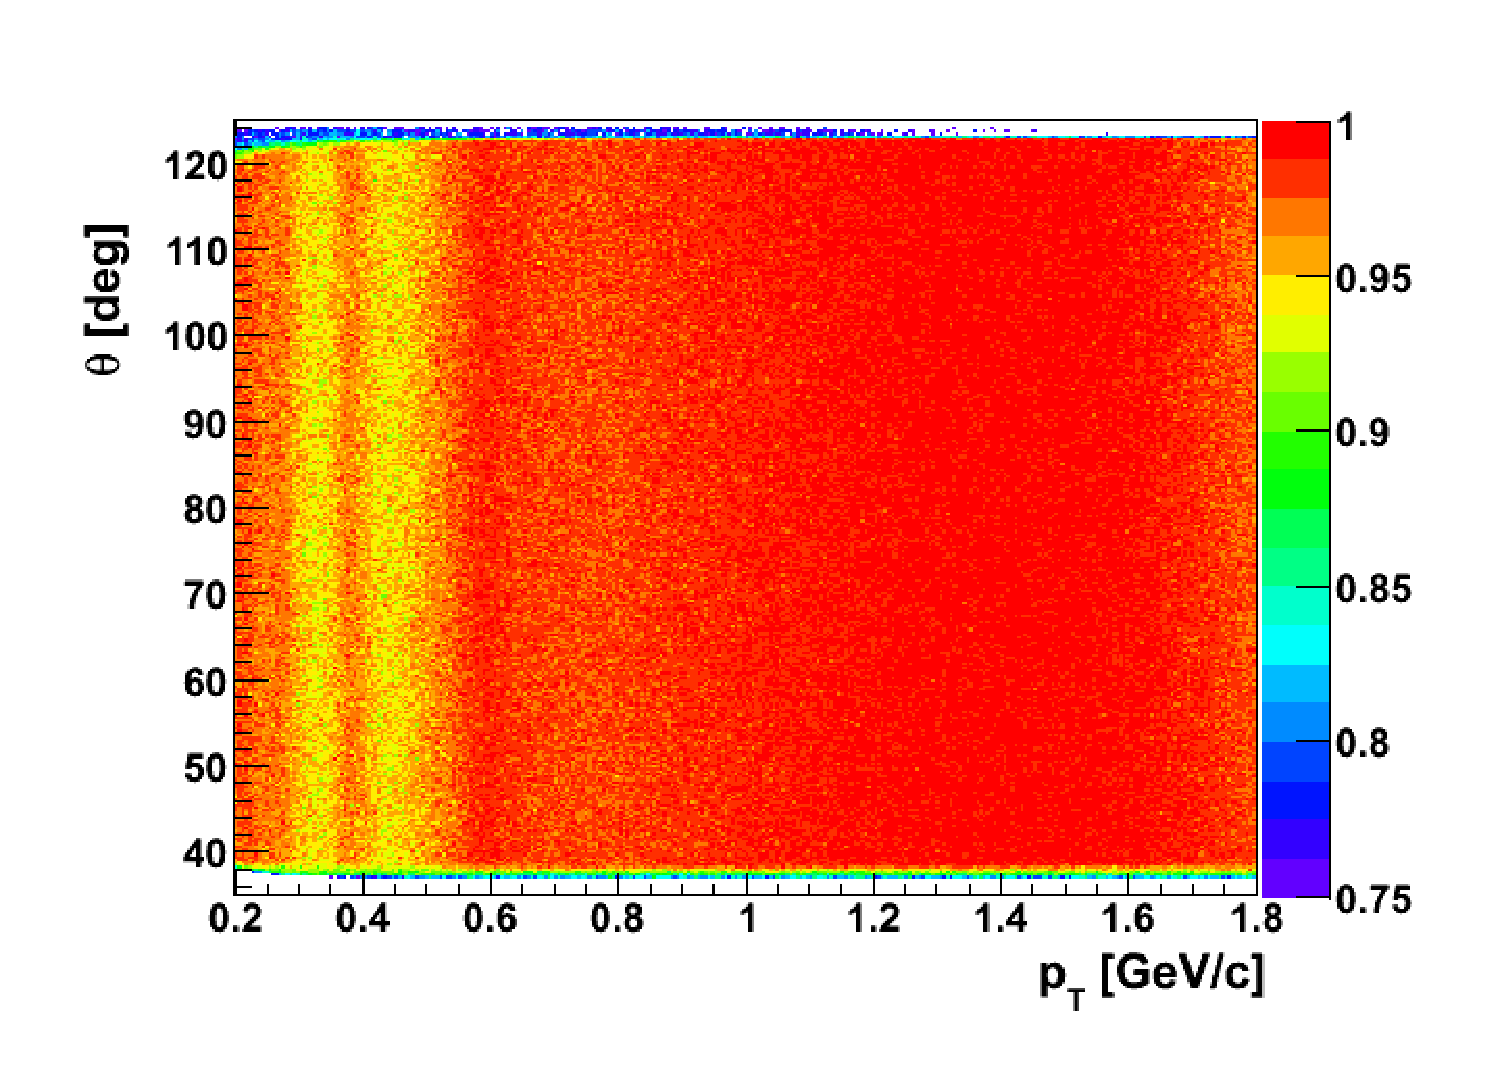
\includegraphics[width=0.49\textwidth]{SVT_2deff_thetapT.eps}
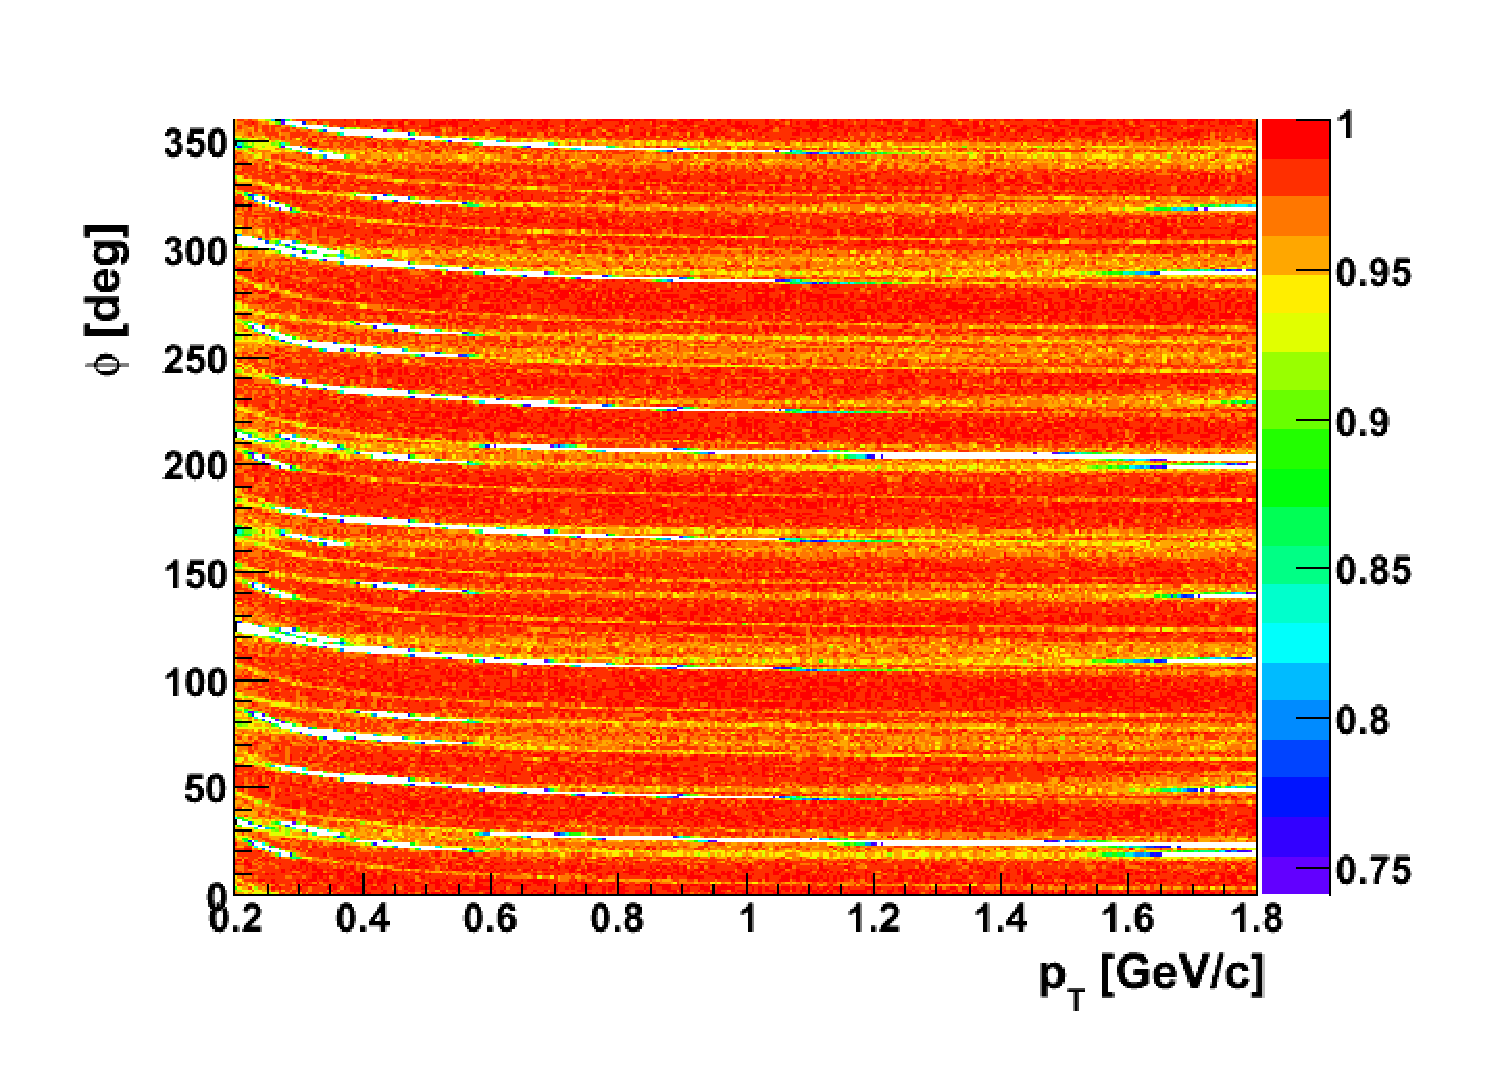
\includegraphics[width=0.49\textwidth]{SVT_2deff_phipT.eps}
\caption{\small{Track finding efficiency as a function of the transverse momentum 
$p_T$ and the polar angle $\theta$ (left) or the azimuthal angle $\phi$ (right).}}
\label{sec_central:pic_eff2d}
\end{figure}
%%%%%%%%%%%%%%%%%%%%%%%%%%%%%%%%%%%%%%%%%%%%%%%%%%%%%%%%%%%%%%%%%%%%%%%%%%%

For a 1-mm long target, the integrated efficiency is:

\begin{equation}
\langle \epsilon \rangle = 94\%.
\end{equation}

\noindent
For a 10-cm long target, this efficiency is around 90\%.  If we use only 3 double 
layers (no redundancy), the inefficiency reaches around 1/3.

\paragraph{Track Fitting:}

Once good track candidates have been identified, the corresponding list of hits is 
sent to the fitter algorithm.  This algorithm is based on the Kalman Filter that we 
described in Section~\ref{sec_KF}.  An important issue is the initialization of the 
state vector and its corresponding covariance matrix.  An analytic estimation of 
$\vec{x}$ is obtained assuming the track is a helix, the solenoid field being quite 
homogeneous across the entire BST.  The initial covariance matrix we choose is 
diagonal, with \emph{relatively} large values for the diagonal terms: around 2~mm for 
the $z$ uncertainty, 1$^\circ$ for $\phi$, 40~MeV for $p_x$ and $p_y$, and 100~MeV 
for $p_z$.  We also introduced a $p_T$ dependence on these terms to take into account 
the uncertainty due to the multiple scattering.  A further improvement would be to 
also introduce a $\theta$ dependence, as small biases were observed for angles close 
to 35$^\circ$ and 125$^\circ$.

Finally, the Kalman Filter is run, starting from the last available measurement, and 
going backwards.  It is stopped when it reaches the distance of closest approach to 
the beam axis, the corresponding point defining the \emph{vertex} of the current 
track.

\subsubsection{Tracking Performance}

The resolutions in $p_T$, $\theta$, $\phi$, and $z$ have been obtained using proton 
tracks at 90$^\circ$.  Because of the multiple scattering, these resolutions depend 
on the transverse momentum, and we used the following expressions to fit the different 
distributions:

\begin{equation}
\sigma_{p_T}/p_T = \sqrt{\left(\sigma_{1,p}\times p\right)^2
+\left(\frac{\sigma_{2,p}}{p\beta}\right)^2}
\end{equation}

\begin{equation}
\sigma_{\theta} = \sqrt{\left(\sigma_{1,\theta}\right)^2
+\left(\frac{\sigma_{2,\theta}}{p\beta}\right)^2}
\end{equation}

\begin{equation}
\sigma_{\phi} = \sqrt{\left(\sigma_{1,\phi}\times p\right)^2
+\left(\frac{\sigma_{2,\phi}}{p\beta}\right)^2}
\end{equation}

\begin{equation}
\sigma_{z} = \sqrt{\left(\sigma_{1,z}\times p\right)^2
+\left(\frac{\sigma_{2,z}}{p\beta}\right)^2}.
\end{equation}

\noindent
The 8 $\sigma_{i,X}$ extracted from the fits are summarized in 
Table~\ref{sec_central:table_resol}.  We see that the original requirements from 
Table~\ref{intro_requirements} are satisfied, even if we are at the upper limit for 
the $\theta$ resolution.

%%%%%%%%%%%%%%%%%%%%%%%%%%%%%%%%%%%%%%%%%%%%%%%%%%%%%%%%%%%%%%%%%%%%%%%%%%%
\begin{table}[ht!]
\centering
\begin{tabular}{|c|c|c|}\hline
                   &  $\sigma_1$ &  $\sigma_2$   \\ \hline
$p$                & 2.72\%      &  1.06\% GeV    \\
$\theta$           & 21.6 mrad   &  1.75 mrad GeV  \\
$\phi$             & 4.60 mrad   &  1.50 mrad GeV  \\
$z$                & 2.30 mm     &  0.13 mm GeV    \\ \hline
\end{tabular}
\caption{\small{Resolutions obtained in the central tracker for protons tracks at 
90$^\circ$.}}
\label{sec_central:table_resol}
\end{table}
%%%%%%%%%%%%%%%%%%%%%%%%%%%%%%%%%%%%%%%%%%%%%%%%%%%%%%%%%%%%%%%%%%%%%%%%%%%

The performance obtained with the Kalman Filter algorithm were also compared with 
estimates that can be analytically derived using the MOMRES program~\cite{momres}. 
To do this, we used only tracks with hits in all the double layers. 
Fig.~\ref{sec_central:pic_momrescomparison} shows that very good agreement is found 
between the two estimates, thus giving us confidence in our tracking code.  We can 
also note that the $p_T$ dependence of the obtained resolutions is very close to the 
expected ones (used for the fits).

%%%%%%%%%%%%%%%%%%%%%%%%%%%%%%%%%%%%%%%%%%%%%%%%%%%%%%%%%%%%%%%%%%%%%%%%%%%
\begin{figure}[ht!]
\centering
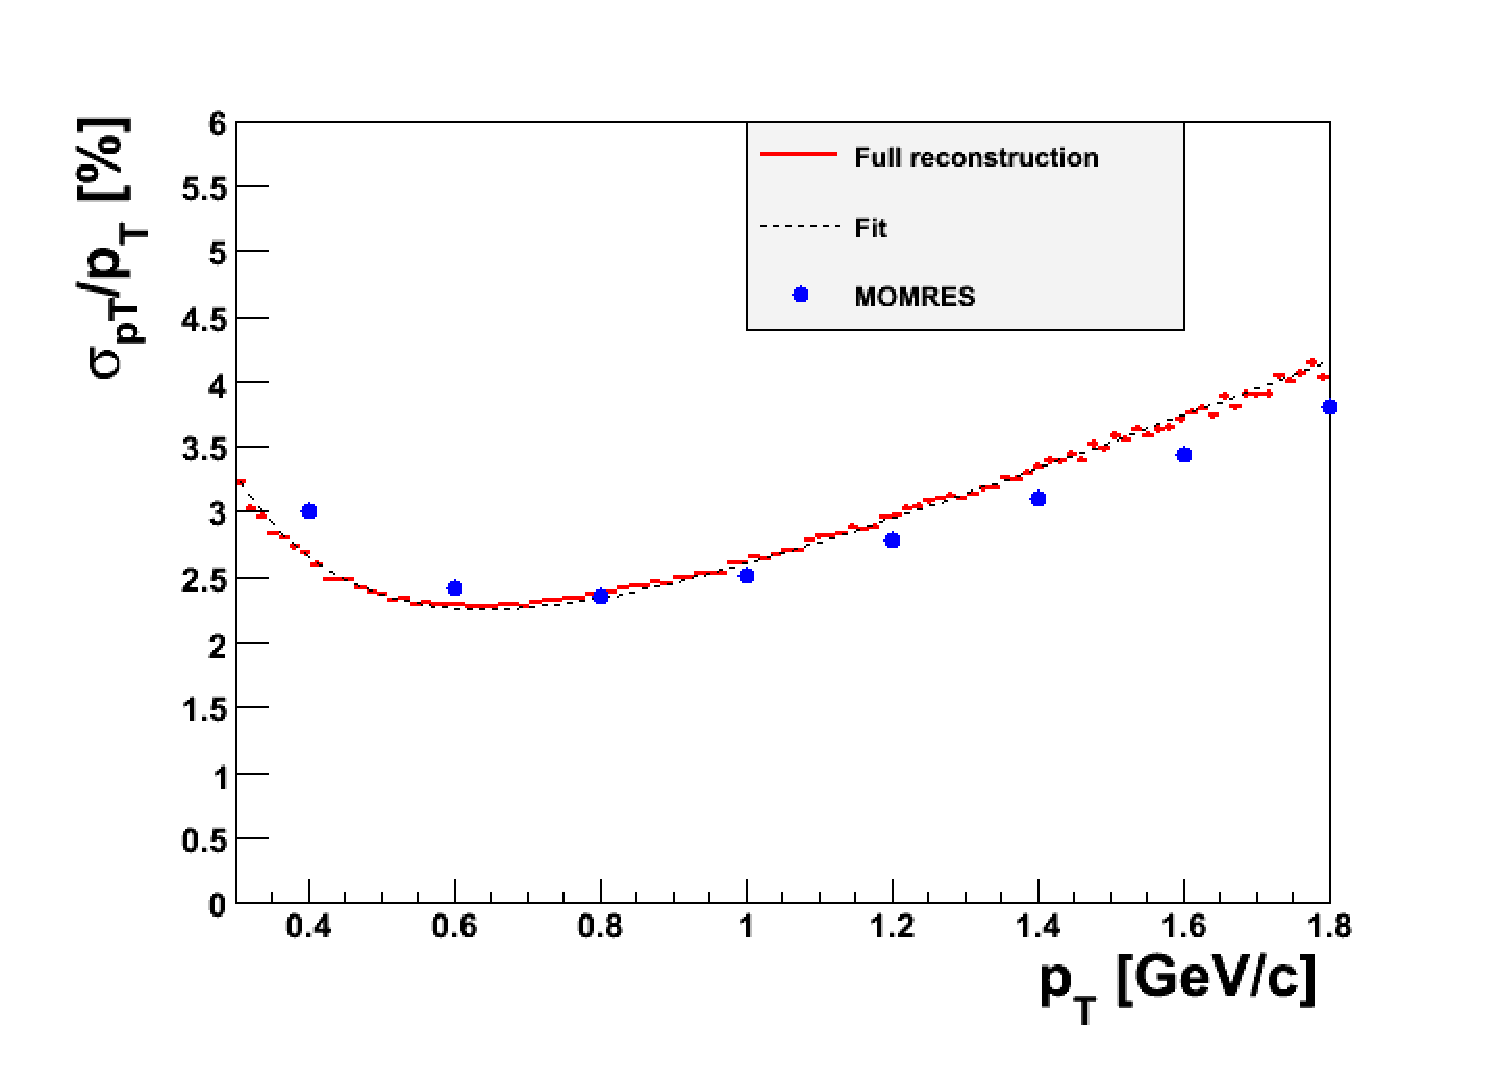
\includegraphics[width=0.49\textwidth]{sigmaptopt_VS_pT_SVTreal_theta60_4outof4_withfit.eps}
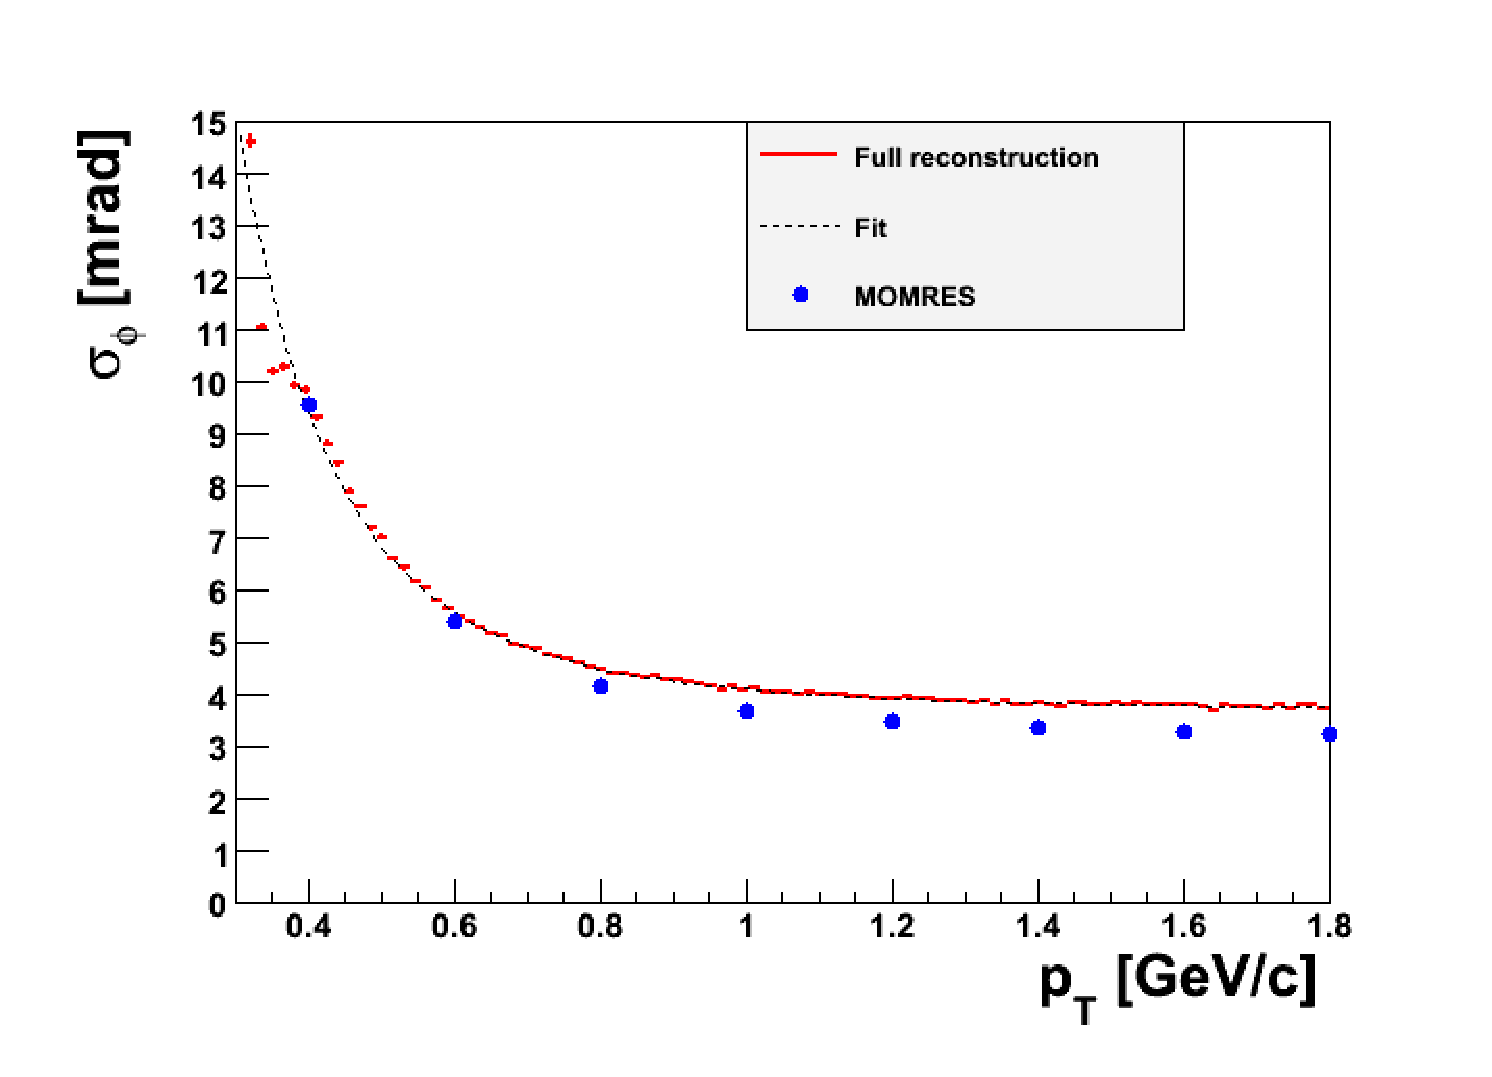
\includegraphics[width=0.49\textwidth]{sigmaphi_VS_pT_SVTreal_theta60_4outof4_withfit.eps}
\caption{\small{Comparison of the resolution in $p_T$ (left) and $\phi$ (right) 
obtained with the full reconstruction code and with the MOMRES program (proton tracks 
at $\theta$ = 60$^\circ$).}}
\label{sec_central:pic_momrescomparison}
\end{figure}
%%%%%%%%%%%%%%%%%%%%%%%%%%%%%%%%%%%%%%%%%%%%%%%%%%%%%%%%%%%%%%%%%%%%%%%%%%%

Finally, Table~\ref{sec_central:table_resolangle} shows the effect of the maximum 
strip angle on the resolutions, using the sample of tracks that has been used for 
the MOMRES comparison.  We see that the $\theta$ resolution can be improved 
significantly by using a larger angle, without significantly affecting the $p_T$ and 
$\phi$ resolutions.  However, a larger crossing angle will increase the 
reconstruction of fake tracks in the presence of background, which still needs to be 
quantified.

%%%%%%%%%%%%%%%%%%%%%%%%%%%%%%%%%%%%%%%%%%%%%%%%%%%%%%%%%%%%%%%%%%%%%%%%%%%
\begin{table}[ht!]
\centering
\begin{tabular}{|c|c|c|c|c|} \hline
$\alpha_{max}$ ($^{\circ}$) & $\sigma_{1,\theta}$ (mrad) & $\sigma_{1,p}$ (\%) & $\sigma_{1,\phi}$ (mrad) & $\sigma_{1,z}$ (mm)  \\ \hline
3    & 18.9   &  2.69  &    4.50   &  2.35  \\
6    & 12.0   &  3.04  &    5.09   &  1.43  \\
12   & 9.77   &  3.26  &    5.48   &  1.12  \\
15   & 8.74   &  4.05  &    6.66   &  0.93  \\ \hline
\end{tabular}
\caption{\small{Evolution of the resolutions with the maximum strip angle 
$\alpha_{max}$.}}
\label{sec_central:table_resolangle}
\end{table}
%%%%%%%%%%%%%%%%%%%%%%%%%%%%%%%%%%%%%%%%%%%%%%%%%%%%%%%%%%%%%%%%%%%%%%%%%%%

\subsubsection{Effect of the Background}

Background hits in the BST can degrade the tracking resolution, and produce fake 
tracks that will complicate the data analysis.  The first case happens when a fake 
hit is accidentally close to a good one, creating a \emph{sister} track that is 
similar to the original one.  But thanks to the good spatial resolution of the BST, 
only very close sister tracks can pass all the tracking filters (including a final 
$\chi^2$ cut), so that the effect on the resolution is very limited.  The creation 
of purely fake tracks, on the other hand, can be more problematic, and needs precise 
simulation on the background rate to be estimated.

The total number of tracks reconstructed in the BST for single particle events with 
uncorrelated background is presented in Fig.~\ref{sec_central:pic_background}.  We 
see that below 100~MHz per BST layer, the number of reconstructed tracks is rather 
limited, but tends to increase more rapidly above 100~MHz.  A detailed analysis shows 
that below this critical rate, additional tracks are mainly sister tracks, whereas 
they are essentially fakes above, when the density of hits is high enough.

%%%%%%%%%%%%%%%%%%%%%%%%%%%%%%%%%%%%%%%%%%%%%%%%%%%%%%%%%%%%%%%%%%%%%%%%%%%
\begin{figure}[ht!]
\centering
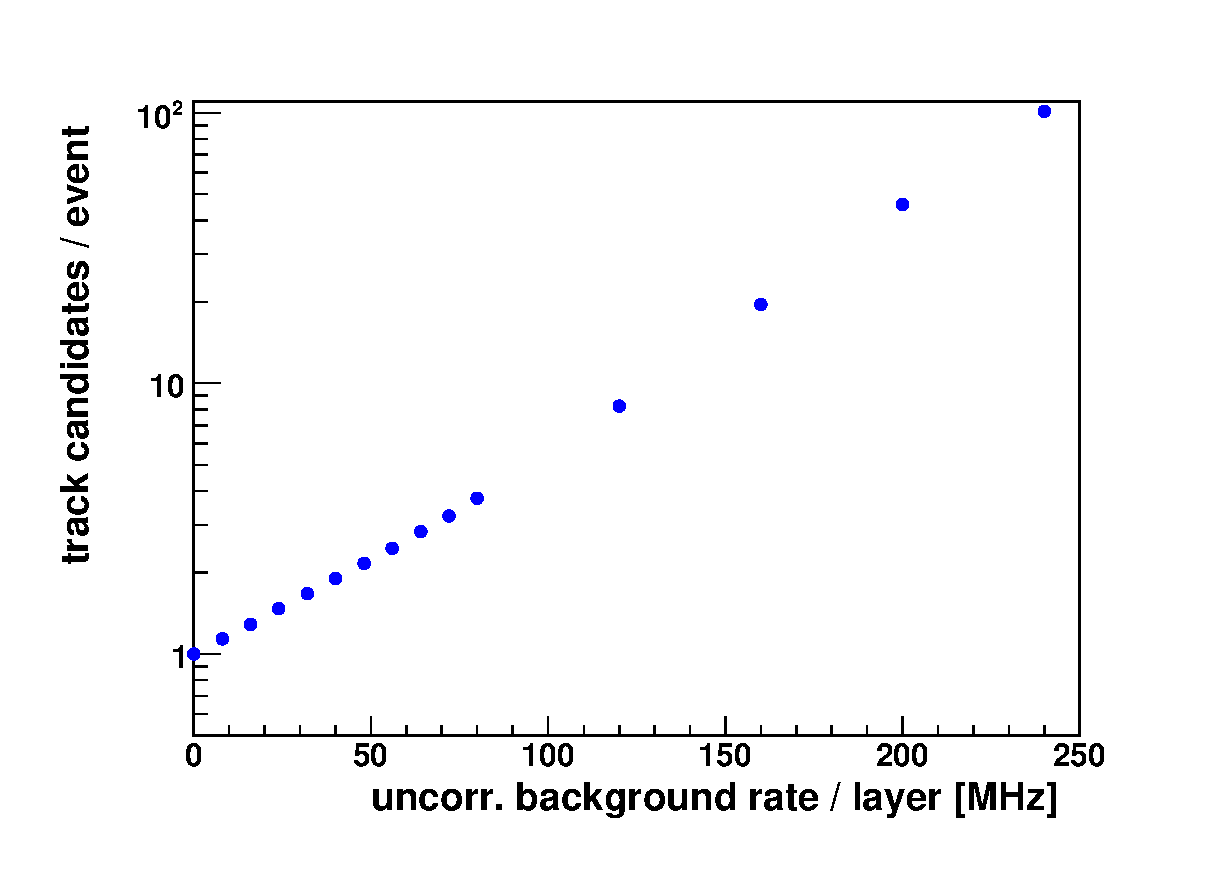
\includegraphics[width=0.7\textwidth]{SVT_trackcand_vs_rate.eps}
\caption{\small{Number of reconstructed tracks for single track events as a function 
of the (uncorrelated) background rate in the BST (see text for details).}}
\label{sec_central:pic_background}
\end{figure}
%%%%%%%%%%%%%%%%%%%%%%%%%%%%%%%%%%%%%%%%%%%%%%%%%%%%%%%%%%%%%%%%%%%%%%%%%%%

More detailed simulations were done using GEANT3 and GEANT4 they indicated that, 
with a luminosity of 10$^{35}$~cm$^{-2}$s$^{-1}$, the background rates do not 
exceed 60~MHz in the BST, i.e. well below the critical 100~MHz limit.  But they 
also showed that the background is slightly correlated, so a few fake tracks are 
indeed seen, as illustrated in Fig.~\ref{sec_central:pic_dvcs}.  However, the 
Central Time-Of-Flight (CTOF) allows for rejection of some of them (see 
Fig.~\ref{sec_central:pic_dvcs} left), thanks to its very good time resolution.  
The remaining tracks have almost the same momentum as the original one (\emph{sister} 
tracks, see Fig.~\ref{sec_central:pic_dvcs} right).  Using a merging algorithm for 
these tracks (to be written), the overall reconstructed events will be clean enough 
for most of the data analyses.

%%%%%%%%%%%%%%%%%%%%%%%%%%%%%%%%%%%%%%%%%%%%%%%%%%%%%%%%%%%%%%%%%%%%%%%%%%%
\begin{figure}[ht!]
\centering
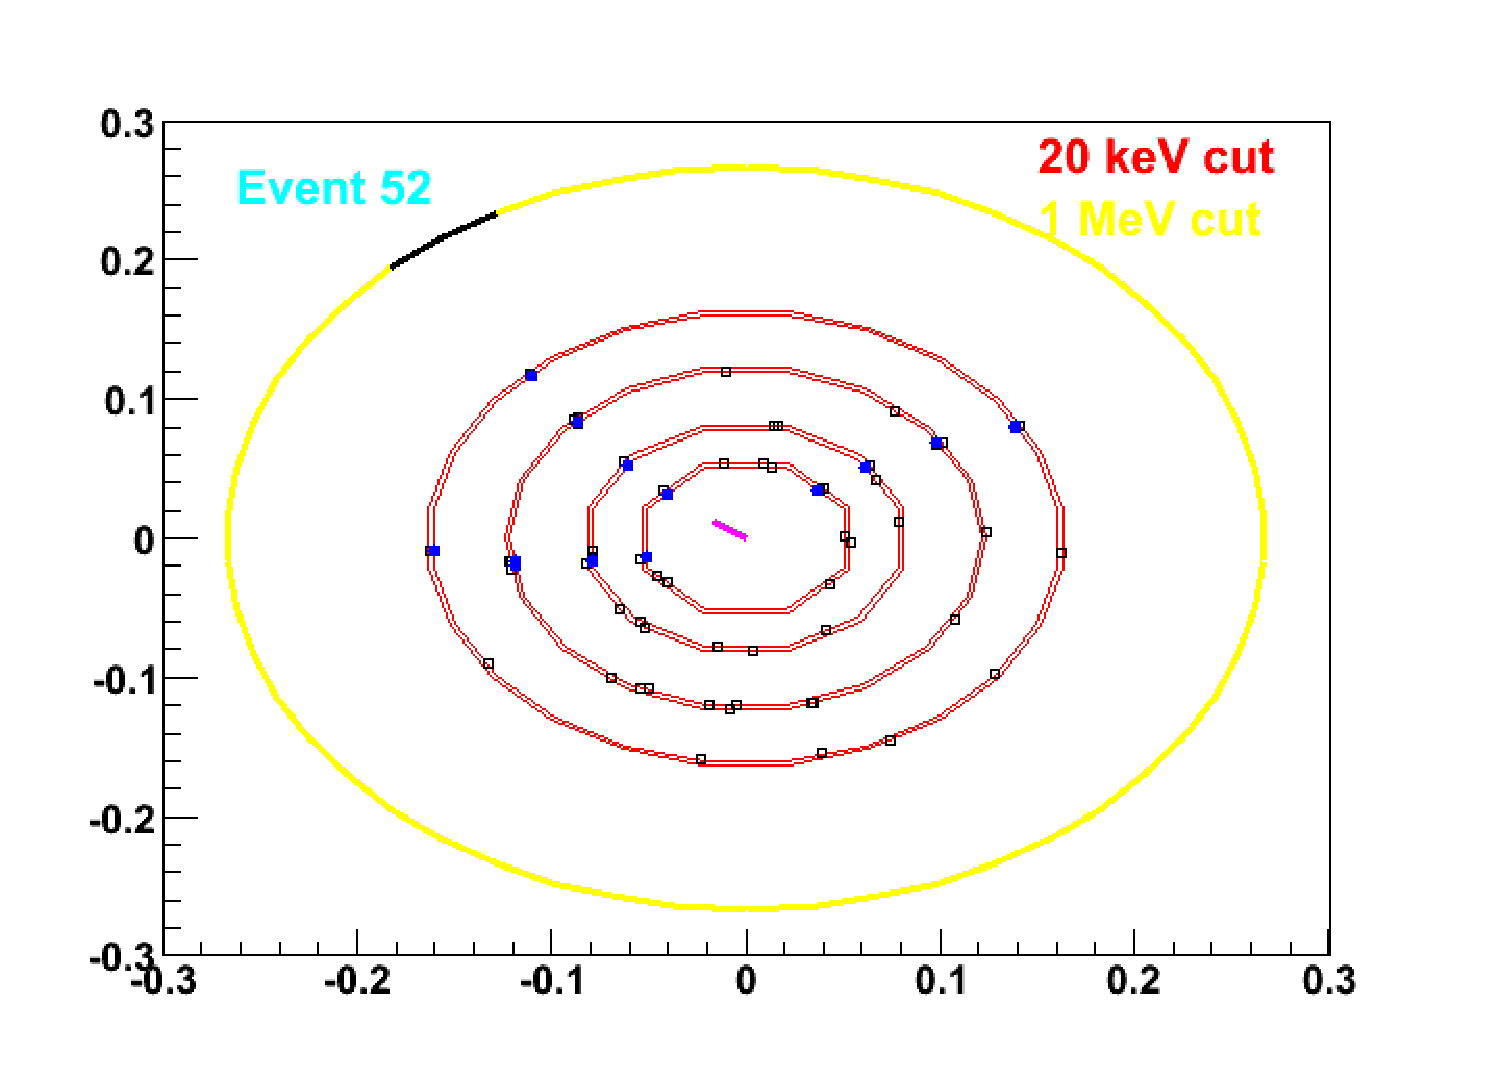
\includegraphics[width=0.49\textwidth]{EvtDisplay_fullLumi_newDVCS_event52_20keVcut_ctof_1MeVcut.eps}
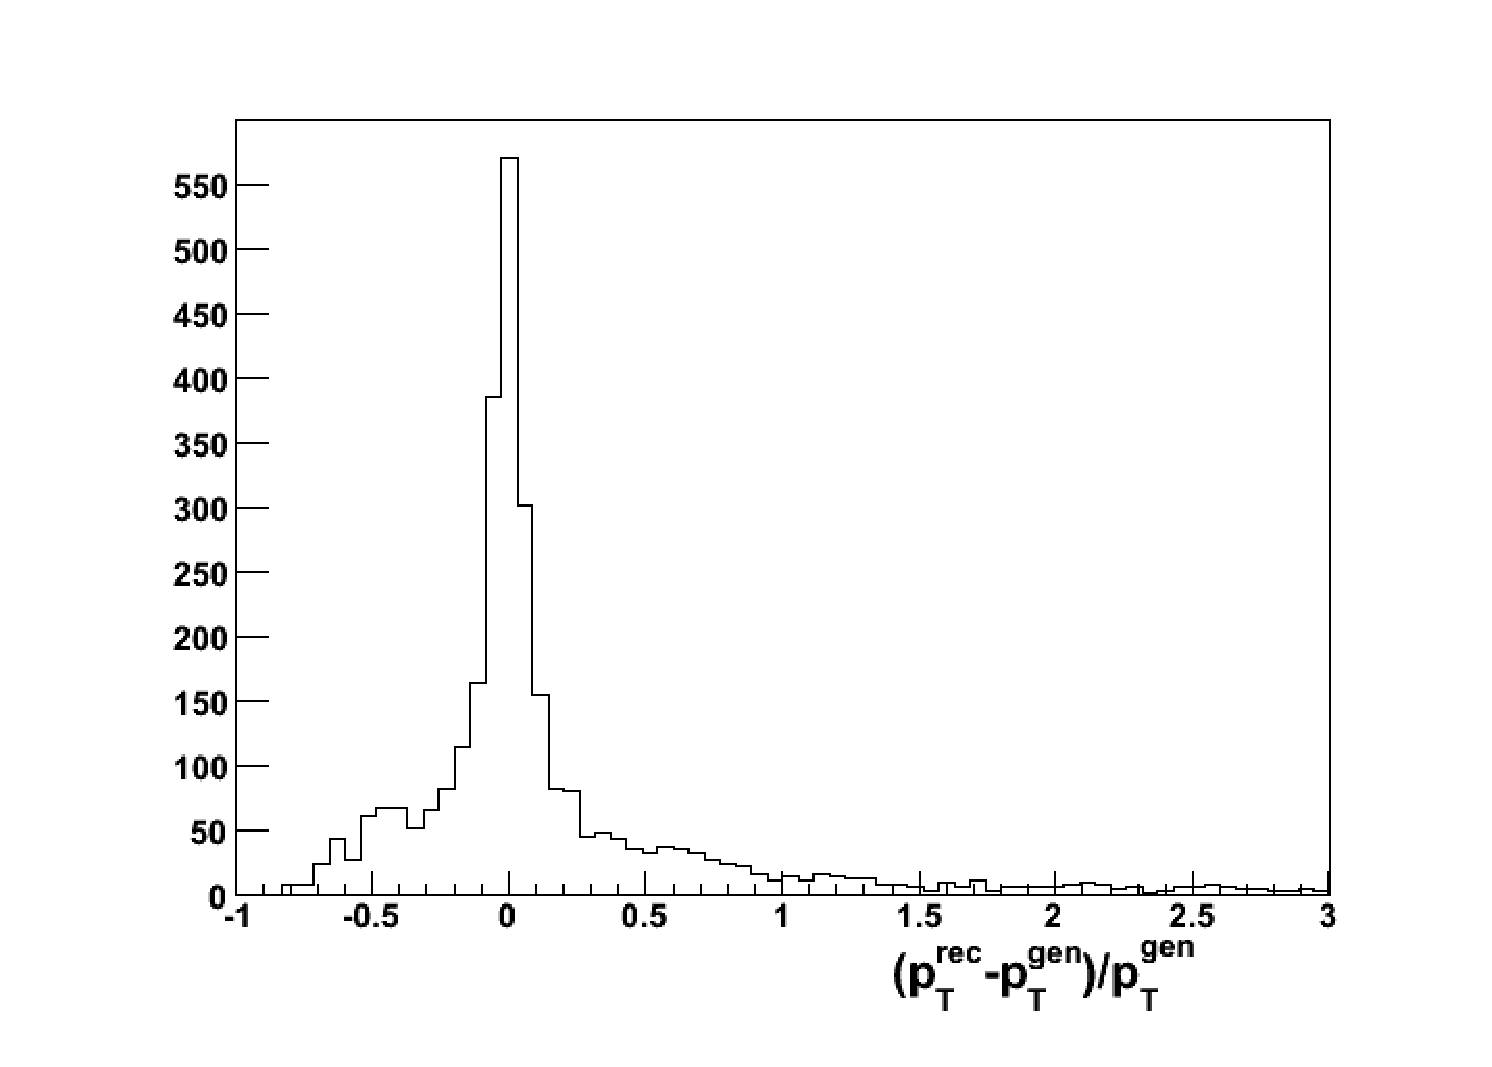
\includegraphics[width=0.49\textwidth]{ptrecons_Edepgt20keV.eps}
\caption{\small{(Left): DVCS event generated with GEANT4 at full luminosity.  The 
proton track (indicated by the pink line) has been correctly identified.  Two fake 
tracks are also visible, but can be rejected using the CTOF information. (Right): 
reconstructed momentum of tracks from DVCS events. On average, three tracks per event 
are reconstructed, most of them are very close to the original one.}}
\label{sec_central:pic_dvcs}
\end{figure}
%%%%%%%%%%%%%%%%%%%%%%%%%%%%%%%%%%%%%%%%%%%%%%%%%%%%%%%%%%%%%%%%%%%%%%%%%%%

\subsubsection{Misalignments}

All the resolutions and performances presented up to now assume a perfectly aligned 
BST.  In practice, many reasons -- from manufacturing to installation -- can 
introduce misalignments~\cite{2008-009}, thus degrading the resolution, not to 
mention introducing systematic shifts in momentum or angles.  To study these effects, 
we studied the use of different geometrical parameters in the track generation and 
the track reconstruction routines of Socrat.  For each BST double layer, the following 
parameters can be misaligned:

\begin{itemize}
\item its radius $R$ (expansion/contraction);
\item its global $\phi$ (rotation around the beam axis);
\item its $z$ position (translation along the beam axis).
\end{itemize}

In practice, one specifies the accuracy of the alignment for all these parameters 
(the accuracy can be different between two double layers), and the program generates 
misalignments on Gaussians with the corresponding widths.  The average effect on the 
resolution can then be estimated by running the program many of times to avoid bias 
from particular configurations.  Fig.~\ref{sec_central:pic_misalignR} illustrates the 
effect of misalignment in $R$.  On the left plot, no misalignments are introduced: 
the resolution found is independent of the sample of events, and no systematic shifts 
in momentum are observed.  On the right plot, one can see that a 200~$\mu$m accuracy 
on $R$ has a limited effect on the momentum resolution, but introduces a shift in 
momentum of the order of 0.8\%.

%%%%%%%%%%%%%%%%%%%%%%%%%%%%%%%%%%%%%%%%%%%%%%%%%%%%%%%%%%%%%%%%%%%%%%%%%%%
\begin{figure}[ht!]
\centering
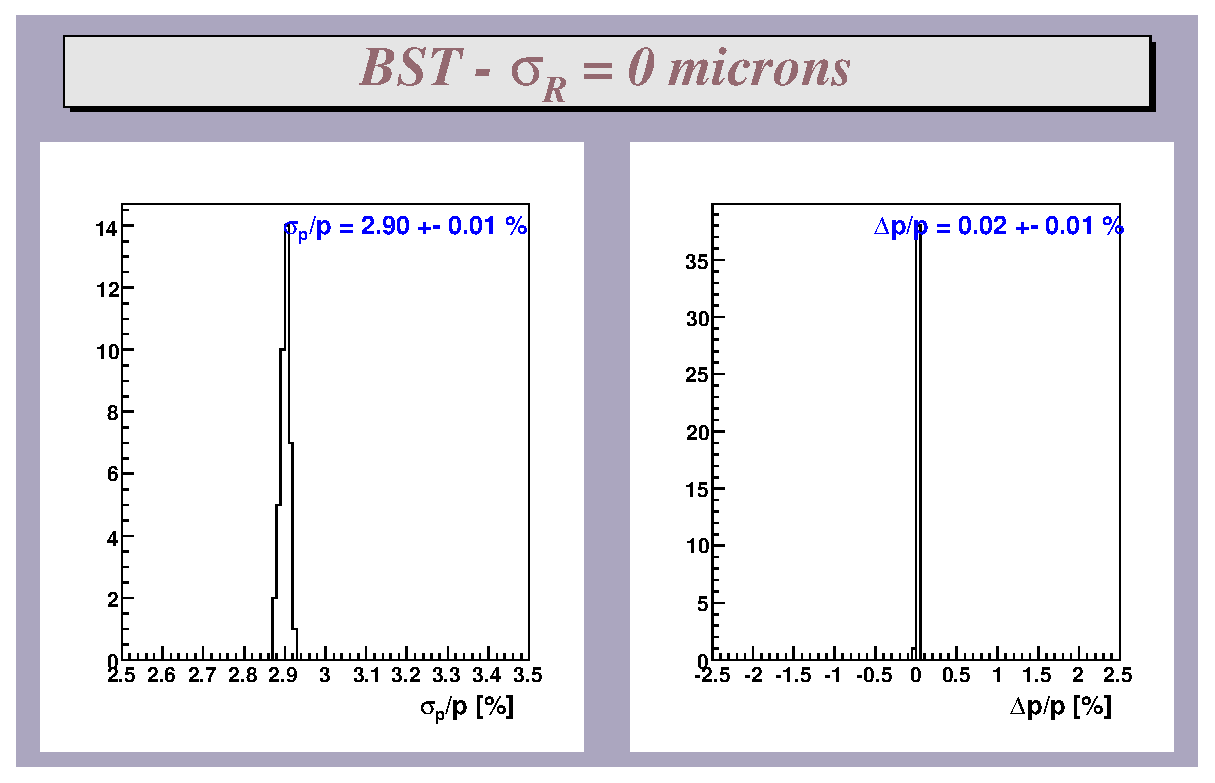
\includegraphics[width=0.49\textwidth]{BST_misalignment_SigmaR0microns.eps}
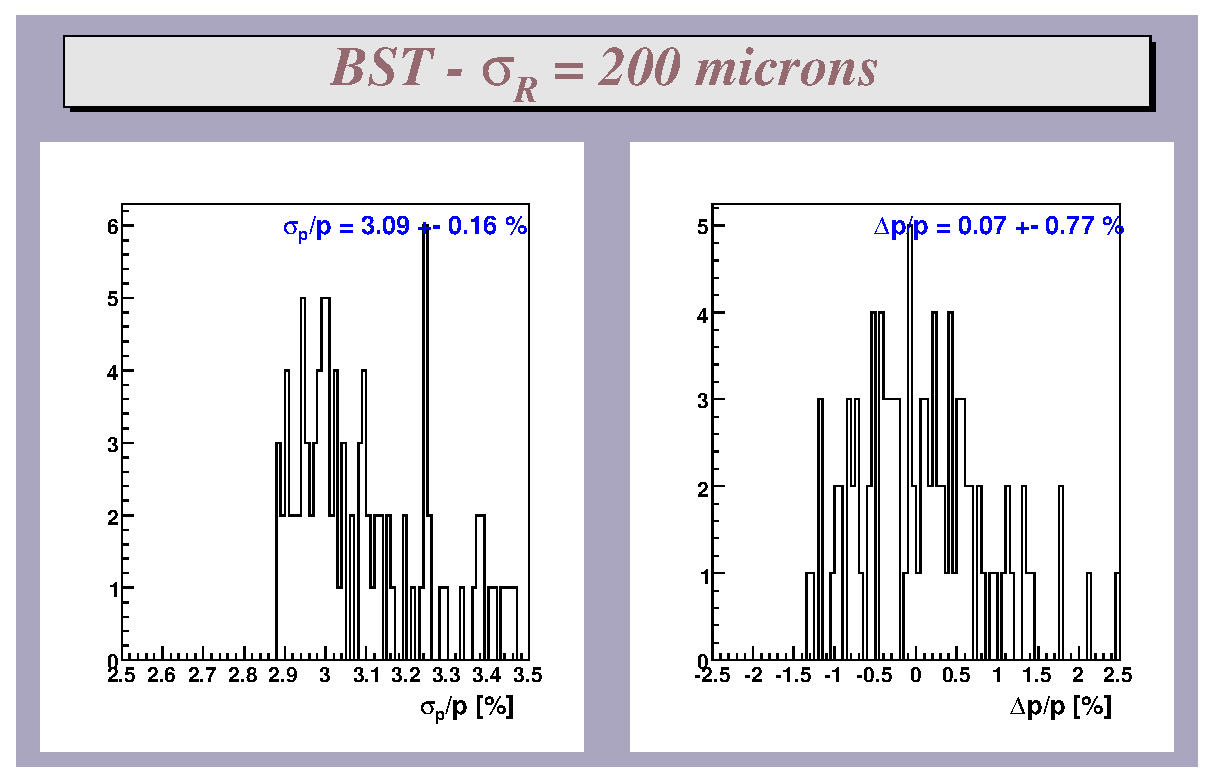
\includegraphics[width=0.49\textwidth]{BST_misalignment_SigmaR200microns.eps}
\caption{\small{Momentum resolution and shift of 0.6~GeV protons at 60$^\circ$ 
without any misalignment (left) and with $R$ misalignment of 200~$\mu$m (right). 
Each entry of these histograms corresponds to a sample of 50k tracks, and a setup 
with misalignments randomly generated with a Gaussian of 0 and 200~$\mu$m widths,
respectively.}}
\label{sec_central:pic_misalignR}
\end{figure}
%%%%%%%%%%%%%%%%%%%%%%%%%%%%%%%%%%%%%%%%%%%%%%%%%%%%%%%%%%%%%%%%%%%%%%%%%%%

As this shift is the largest effect of misalignment, it has been studied as a 
function of misalignments in $R$ and $\phi$ (the misalignment in $z$ has almost no 
effect on momentum resolution, and limited effect on other track parameters).  These 
studies are summarized in Fig.~\ref{sec_central:pic_misalignRPhi}.  If we want to 
keep the momentum shift below 0.5\%, the plots tell us we need an accuracy:

\begin{itemize}
\item better than 100 microns in $R$;
\item better than 0.2 mrad in $\phi$.
\end{itemize}

%%%%%%%%%%%%%%%%%%%%%%%%%%%%%%%%%%%%%%%%%%%%%%%%%%%%%%%%%%%%%%%%%%%%%%%%%%%
\begin{figure}[ht!]
\centering
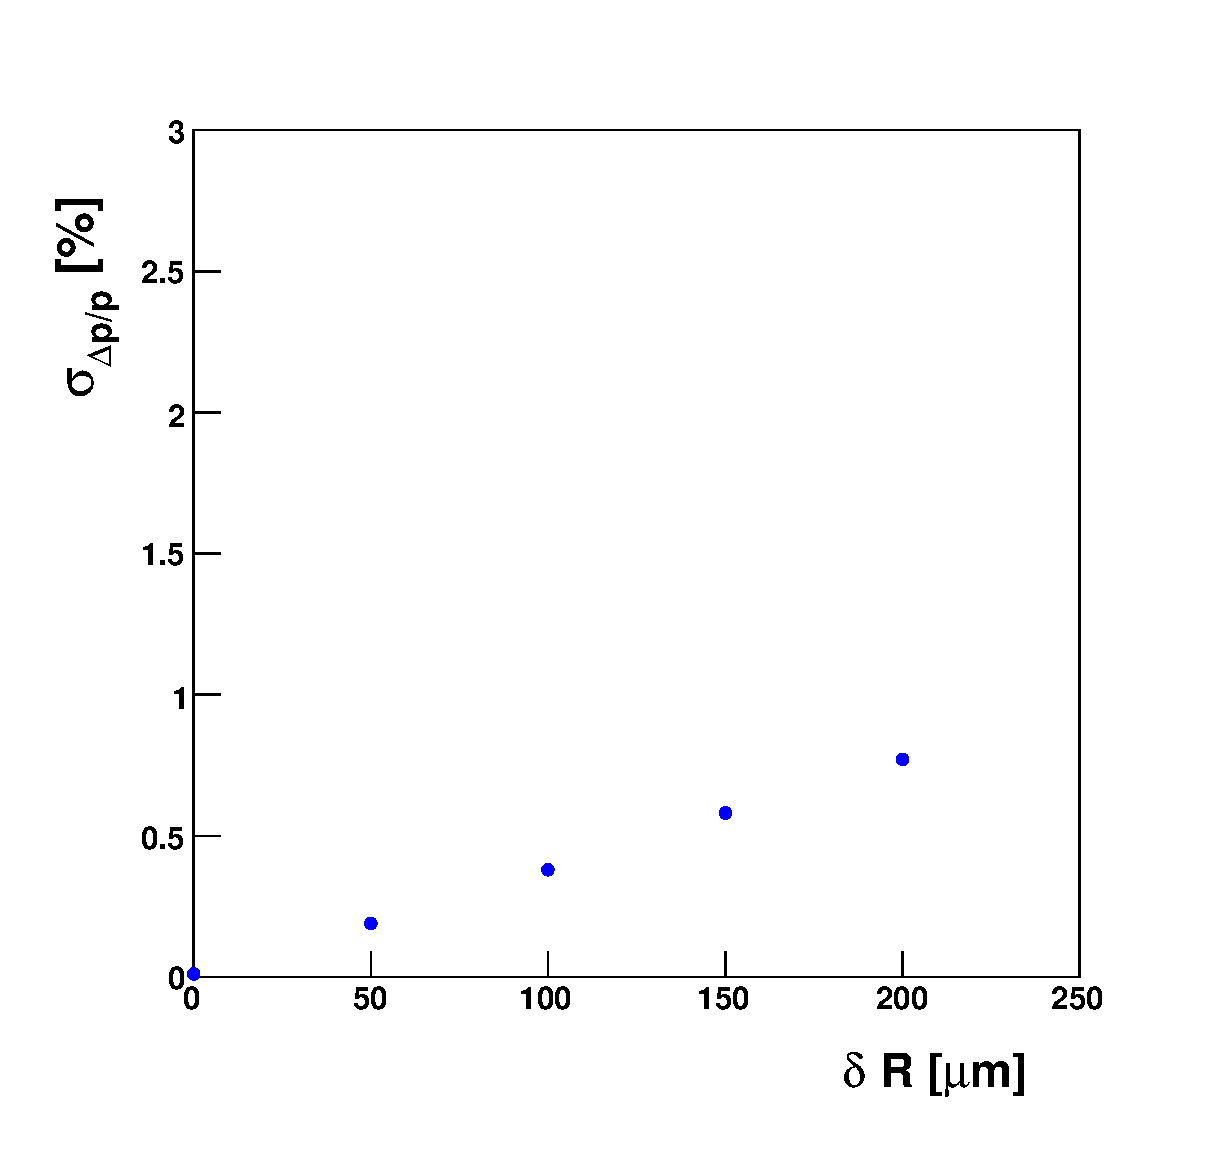
\includegraphics[width=0.49\textwidth]{MomShift_vs_Rmisalign.eps}
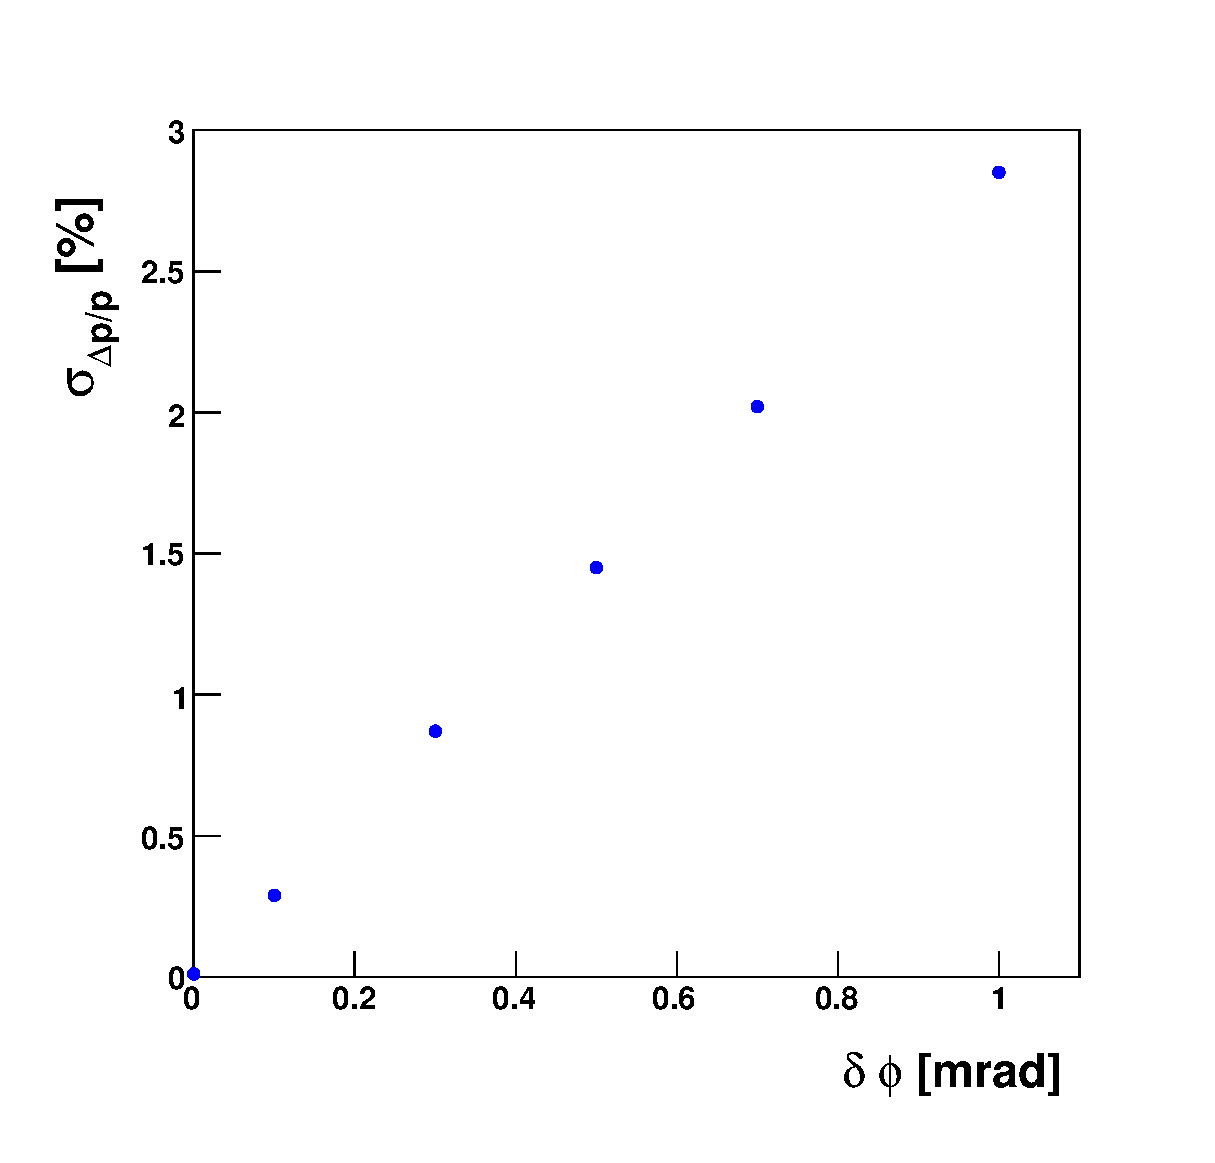
\includegraphics[width=0.49\textwidth]{MomShift_vs_Phimisalign.eps}
\caption{\small{Typical size of the momentum shift as a function of misalignments in 
$R$ (left) and $\phi$ (right) (0.6~GeV protons at 60$^\circ$).}}
\label{sec_central:pic_misalignRPhi}
\end{figure}
%%%%%%%%%%%%%%%%%%%%%%%%%%%%%%%%%%%%%%%%%%%%%%%%%%%%%%%%%%%%%%%%%%%%%%%%%%%

\noindent
These constraints seem to be compatible with what can be reasonably achieved.

Finally, we checked that misalignments in all the variables simultaneously have 
effects that are compatible with the ones obtained with separate misalignments, as 
illustrated in Fig.~\ref{sec_central:pic_misalignRZPhi}.

%%%%%%%%%%%%%%%%%%%%%%%%%%%%%%%%%%%%%%%%%%%%%%%%%%%%%%%%%%%%%%%%%%%%%%%%%%%
\begin{figure}[ht!]
\centering
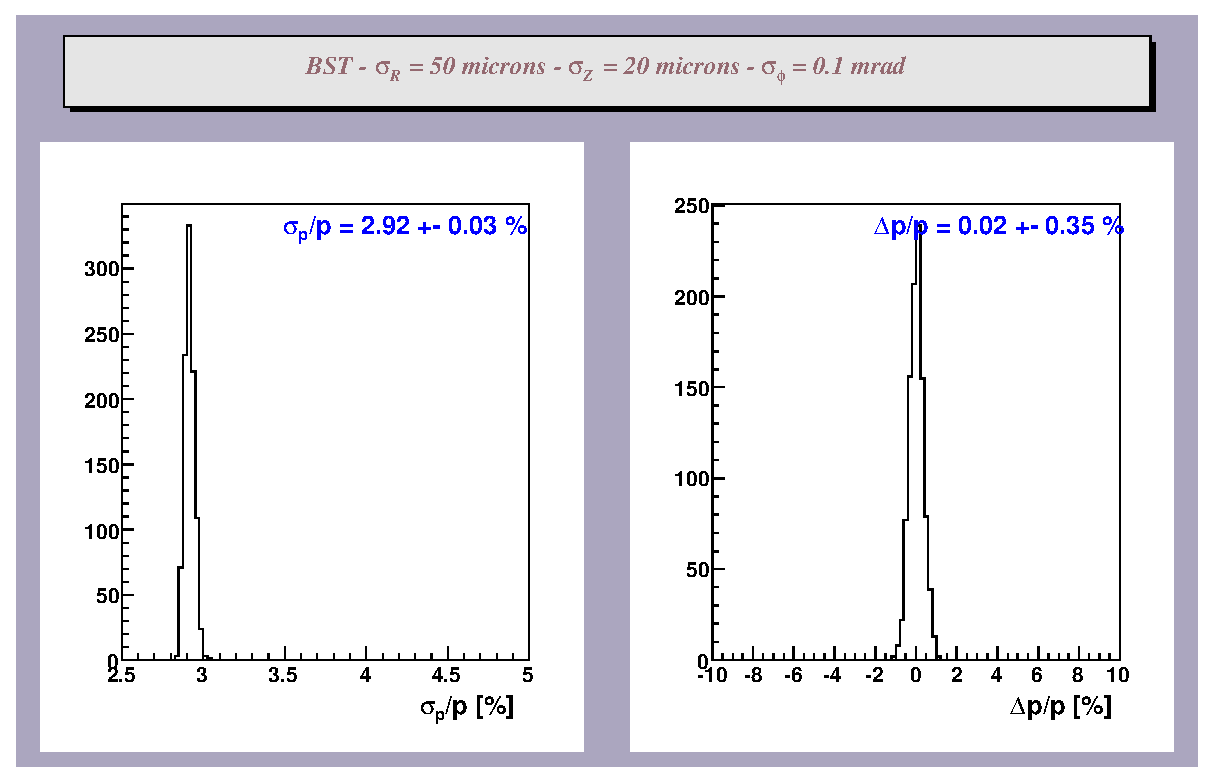
\includegraphics[width=0.49\textwidth]{BST_misalignment_SigmaR50microns_SigmaZ20microns_SigmaPhi01mrad.eps}
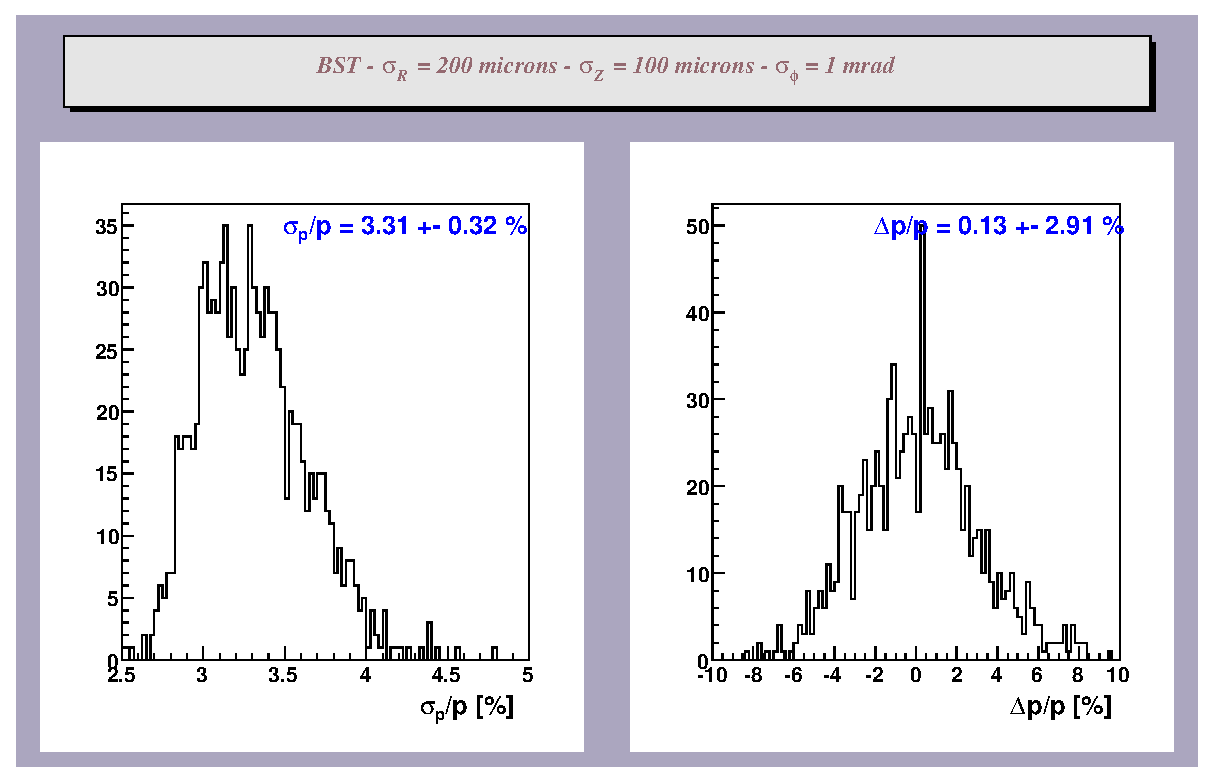
\includegraphics[width=0.49\textwidth]{BST_misalignment_SigmaR200microns_SigmaZ100microns_SigmaPhi1mrad.eps}
\caption{\small{Momentum resolution and shift of 0.6~GeV protons at 60$^\circ$ with 
two different sets of misalignments: $\delta$$R$ = 50~$\mu$m; $\delta$$z$ = 20~$\mu$m; 
$\delta$$\phi$ = 0.1 mrad (left); $\delta$$R$ = 200~$\mu$m; $\delta$$z$ = 100~$\mu$m; 
$\delta$$\phi$ = 1 mrad (right).}}
\label{sec_central:pic_misalignRZPhi}
\end{figure}
%%%%%%%%%%%%%%%%%%%%%%%%%%%%%%%%%%%%%%%%%%%%%%%%%%%%%%%%%%%%%%%%%%%%%%%%%%%

\subsection{Forward Tracking}
\label{sec_forward}

\subsubsection{DC and FST Design}

The FST allows the detection of particles between 5$^\circ$ and 35$^\circ$.  Its 
major component is a set of 36 planes of Drift Chambers, divided in three regions of 
two superlayers each, ensuring highly efficient detection with large redundancy. 
Each region is divided in six sectors of 60$^\circ$, each of them containing six 
planes of 112 wires.  From studies of the current {\tt CLAS} DC, the space resolution 
is expected to be around 250--300~$\mu$m.  The momentum determination will be provided 
by the use of a toroidal magnetic field surrounding Region~2.

The other element of this tracker is the FST, which consists of three double layers of 
silicon strips located between the target and the DC.  Each layer is made with 15 
trapezoids, with stereo strip angles of $\pm$12$^\circ$.  

\subsubsection{Tracking in the DC}

The tracking in the Drift Chambers is performed in three successive steps that will be 
described below:

\begin{itemize}
\item first, we look for combinations of \emph{clusters} that can define a track 
candidate;
\item then we identify a \emph{road} in each of the selected clusters (and solve the 
left-right ambiguity of the corresponding hits);
\item finally we run the Kalman Filter algorithm on the track candidates for which 
roads were successfully identified.
\end{itemize}

\paragraph{Cluster and Track Finding:}

If a particle goes through a DC superlayer, it will leave a collection of hits 
forming a continuous series of wire numbers (e.g. wire number 37 in first plane, 38 
in second, 37 in third, etc.).  The very first step of the tracking is therefore to 
loop over all the hits of an event to find these series (called \emph{clusters}), 
with hits in all the planes of the current superlayer.  To have overall fast and 
efficient tracking, the number of found clusters should be limited, so the occupancy 
in the DC should not exceed a few percent, as illustrated in 
Fig.~\ref{sec_forward:pic_Nclusters}.

%%%%%%%%%%%%%%%%%%%%%%%%%%%%%%%%%%%%%%%%%%%%%%%%%%%%%%%%%%%%%%%%%%%%%%%%%%%
\begin{figure}[ht!]
\centering
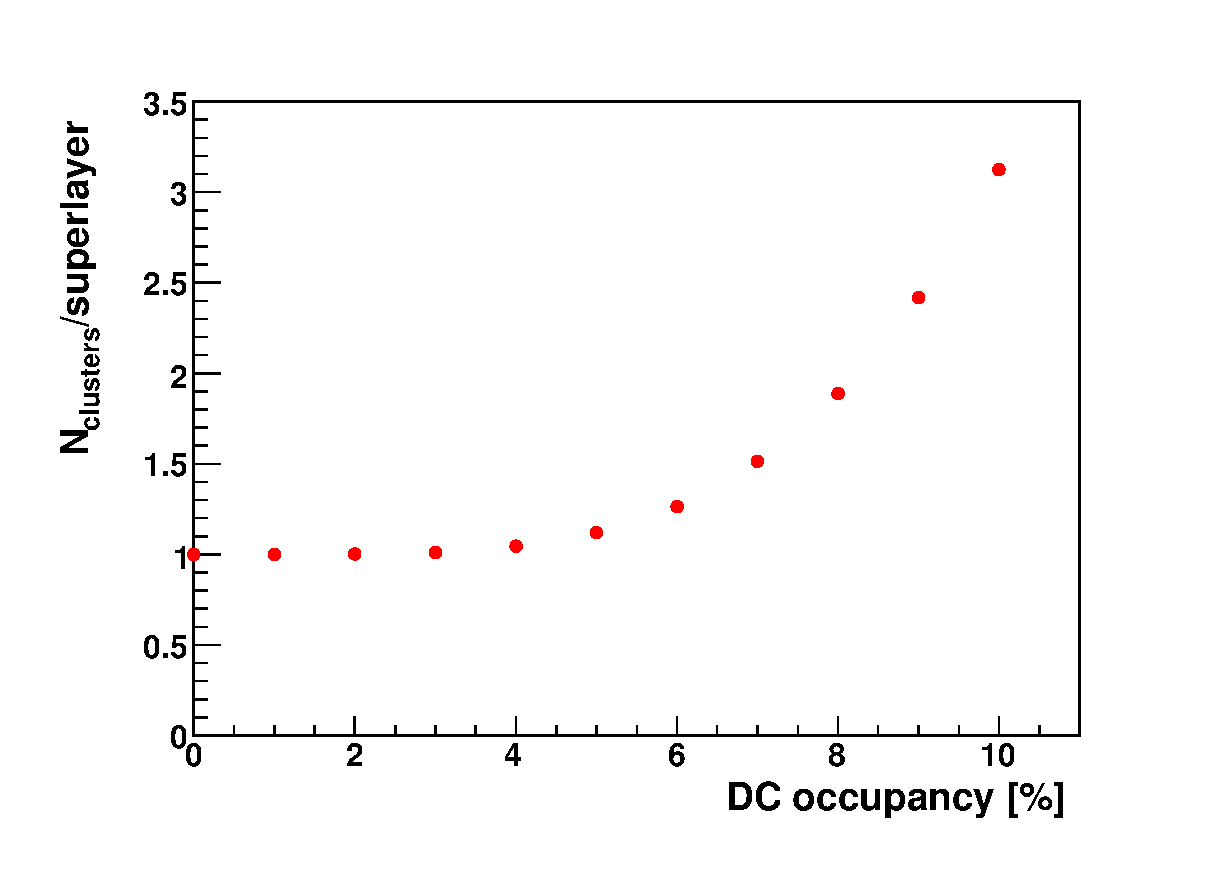
\includegraphics[width=0.7\textwidth]{Ncluster_vs_occupancy.eps}
\caption{\small{Evolution of the number of clusters per DC superlayer for single 
track events with (uncorrelated) background.}}
\label{sec_forward:pic_Nclusters}
\end{figure}
%%%%%%%%%%%%%%%%%%%%%%%%%%%%%%%%%%%%%%%%%%%%%%%%%%%%%%%%%%%%%%%%%%%%%%%%%%%

The next step is to form a \emph{track segment} candidate, that is a combination of 
two close clusters in a given region. for real tracks, the average wire numbers 
$W_1$ and $W_2$ of two consecutive clusters satisfy the inequality 
$|W_1$ - $W_2|$ $<$ $K\times$$W_1$, with $K$ around 0.15.  In practice, we obtained 
a cluster matching efficiency close to 100\% by using:

\begin{equation}
|W_1-W_2| < 0.18 \times W_1 + 5.
\end{equation}

Finally, we look for a combination of track segments in all the DC regions that could 
define a track candidate.  As the number of track segments is limited with the 
expected occupancy, we simply require at this stage that they all are in a single 
sector.  The very few remaining bad candidates will be rejected during the fitting 
procedure.

The result of the track finding is illustrated in 
Fig.~\ref{sec_forward:pic_trackfinding}, which shows the initial distribution of hits 
in the DC, and the final remaining candidates.

%%%%%%%%%%%%%%%%%%%%%%%%%%%%%%%%%%%%%%%%%%%%%%%%%%%%%%%%%%%%%%%%%%%%%%%%%%%
\begin{figure}[ht!]
\centering
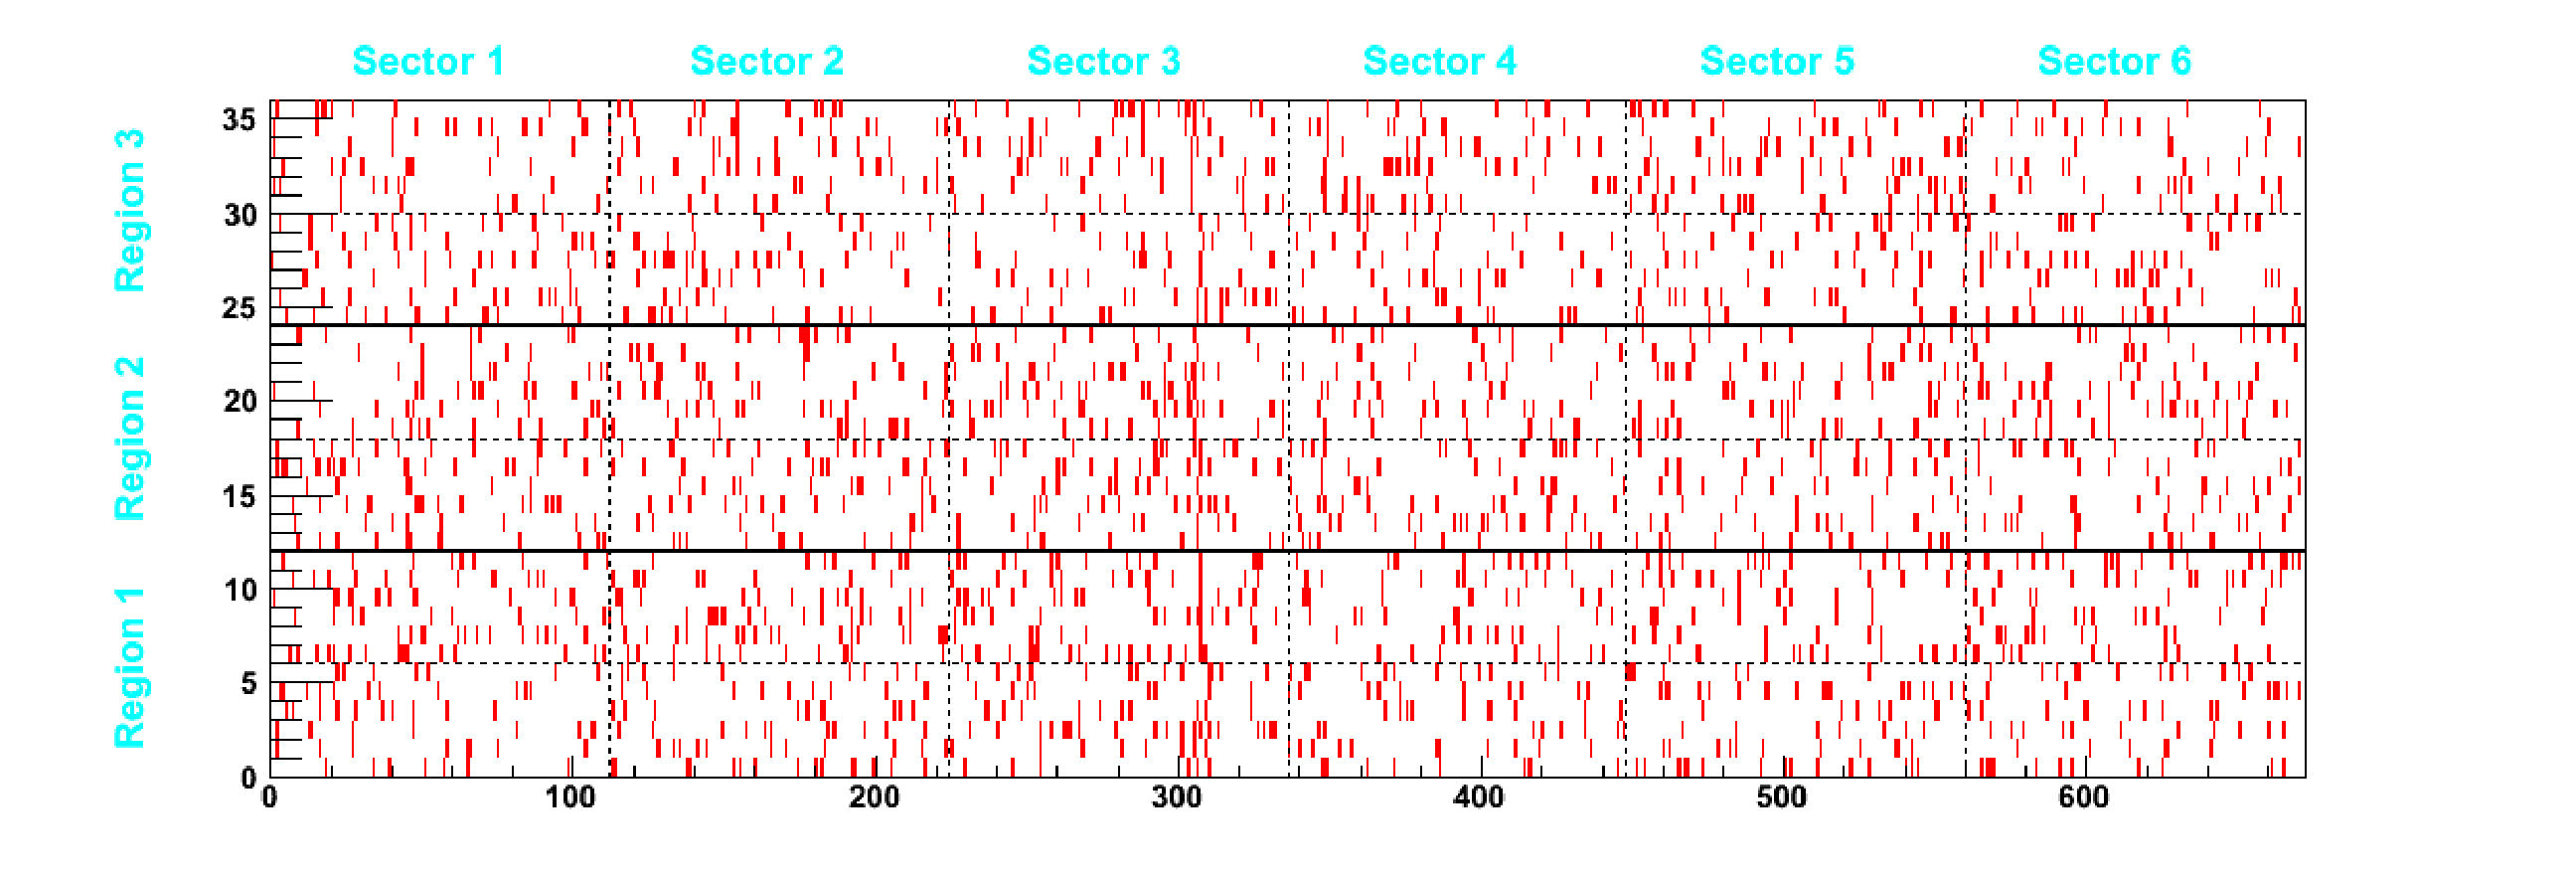
\includegraphics[width=0.6\textwidth]{DC_clusterfinding_step0.eps}
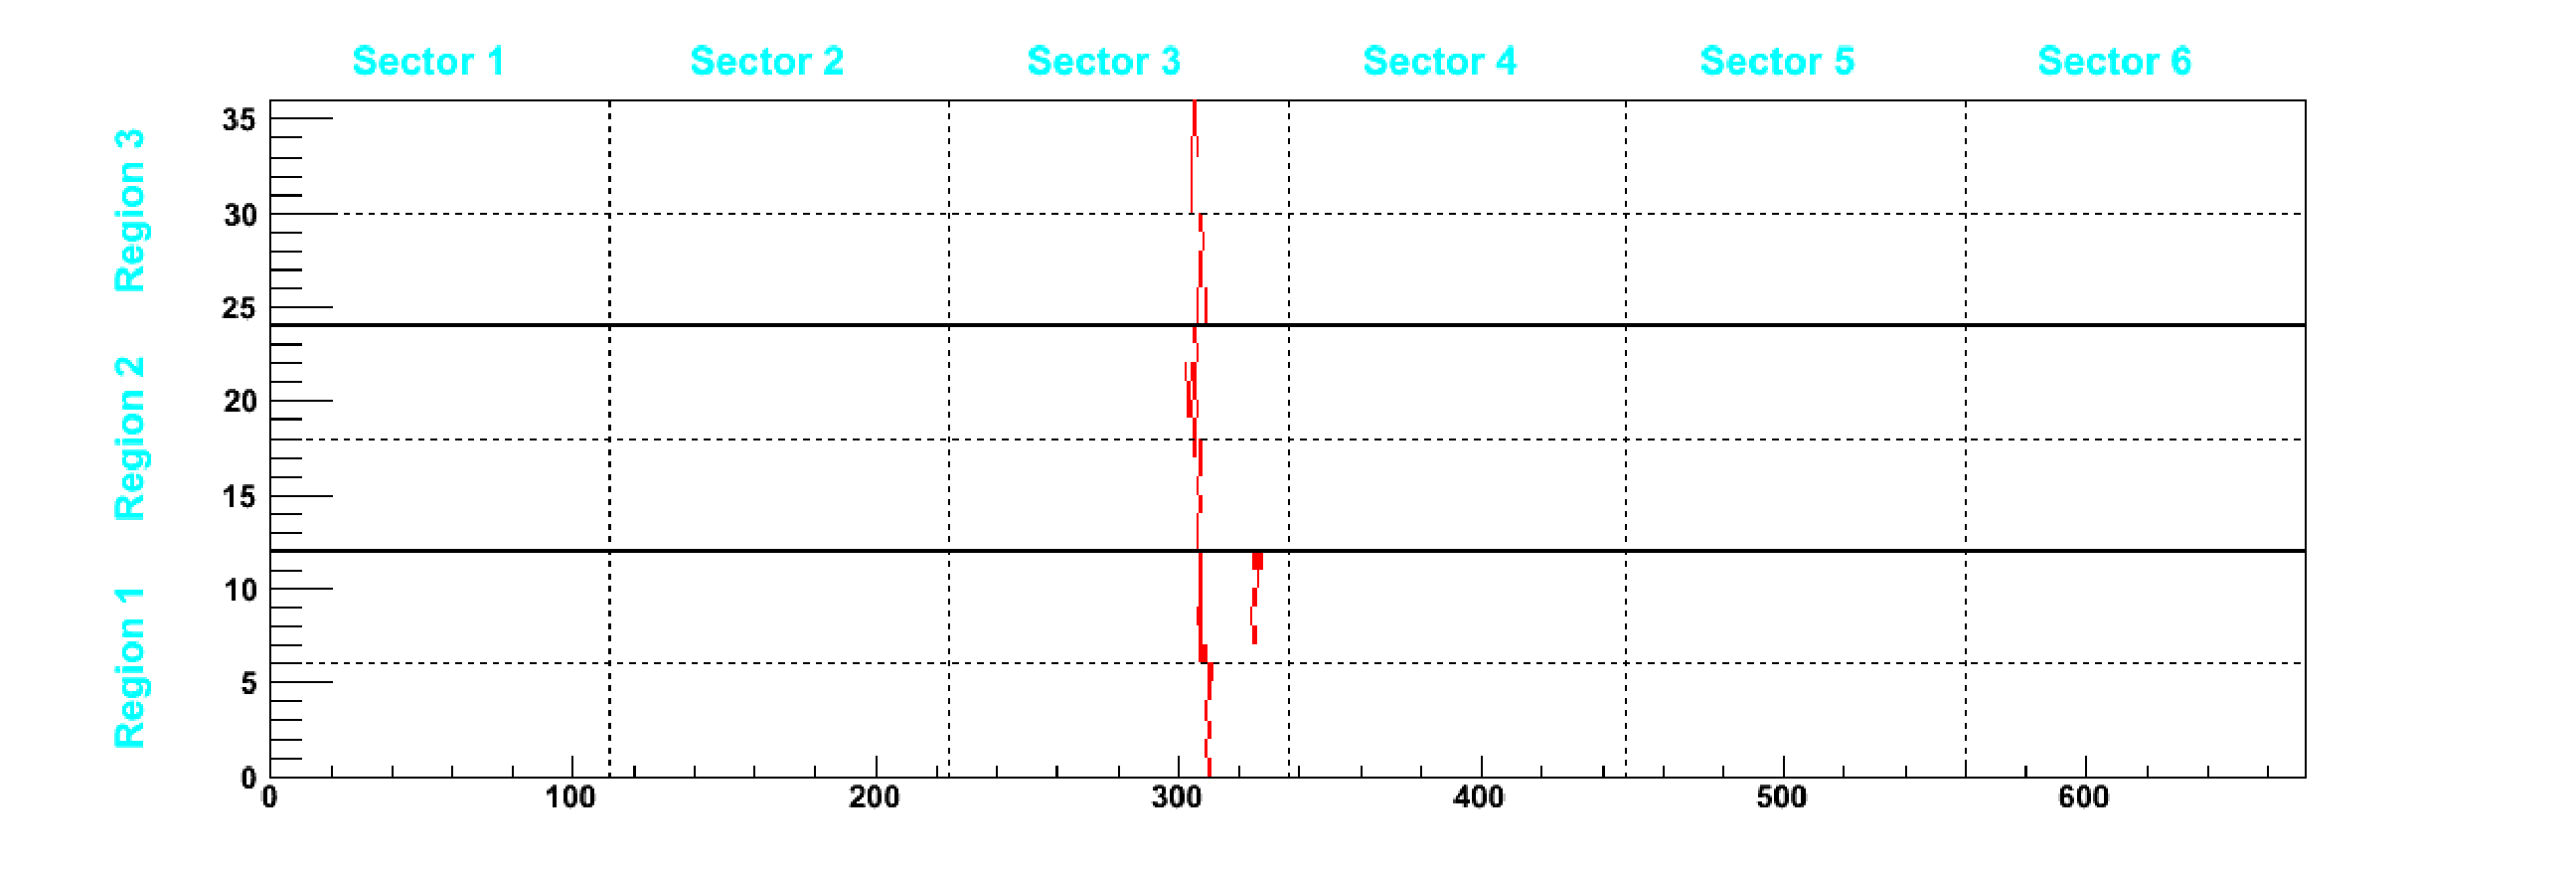
\includegraphics[width=0.6\textwidth]{DC_clusterfinding_step3.eps}
\caption{\small{(Top): distribution of initial hits in all the DC planes (single track 
event with 10\% uncorrelated occupancy); (bottom): remaining track candidates.}}
\label{sec_forward:pic_trackfinding}
\end{figure}
%%%%%%%%%%%%%%%%%%%%%%%%%%%%%%%%%%%%%%%%%%%%%%%%%%%%%%%%%%%%%%%%%%%%%%%%%%%

\paragraph{Road Finding:}

Even without any background, a real cluster cannot be used directly for the fit, as 
left-right ambiguities should be solved.  In the presence of background, a real 
cluster may also contain fake hits that are accidentally close to the real ones.  To 
solve these two problems, we developed the following iterative procedure:

\begin{itemize}
\item we first try to fit each hit combination of a cluster with a straight line, in 
a plane perpendicular to the wire direction.  At this stage, we only use the wire 
position, with an uncertainty corresponding to the drift distance;
\item this preliminary fit allows us to discard some hits (on the edges of the 
cluster), and to solve, for a particular combination, some left-right ambiguities. 
The next iteration uses only the remaining hits, with the real hit position if the
left-right ambiguity has been solved.  The fits are then more and more precise, so 
that more and more ambiguities are solved;
\item after four iterations, all of the remaining ambiguities are solved using the 
latest fit.
\end{itemize}

Note that for the moment, the final road cannot contain more than one hit per plane, 
even if particles with large incidence angle can indeed leave two good hits within 
a single layer.

If the initial track is relatively close to a wire, it is sometimes not possible to 
decide whether it was on the left or on the right: in total, our procedure makes 
the correct decision for 90\% of the hits.  In the presence of background, this 
probability decreases, as a fake hit can ``kill'' a good one, or be close enough to 
be identified as good, and then spoil the fit.  However, this effect is limited, as 
shown in Fig.~\ref{sec_forward:pic_roadsincluster}, proving that our procedure is 
relatively robust.

%%%%%%%%%%%%%%%%%%%%%%%%%%%%%%%%%%%%%%%%%%%%%%%%%%%%%%%%%%%%%%%%%%%%%%%%%%%
\begin{figure}[ht!]
\centering
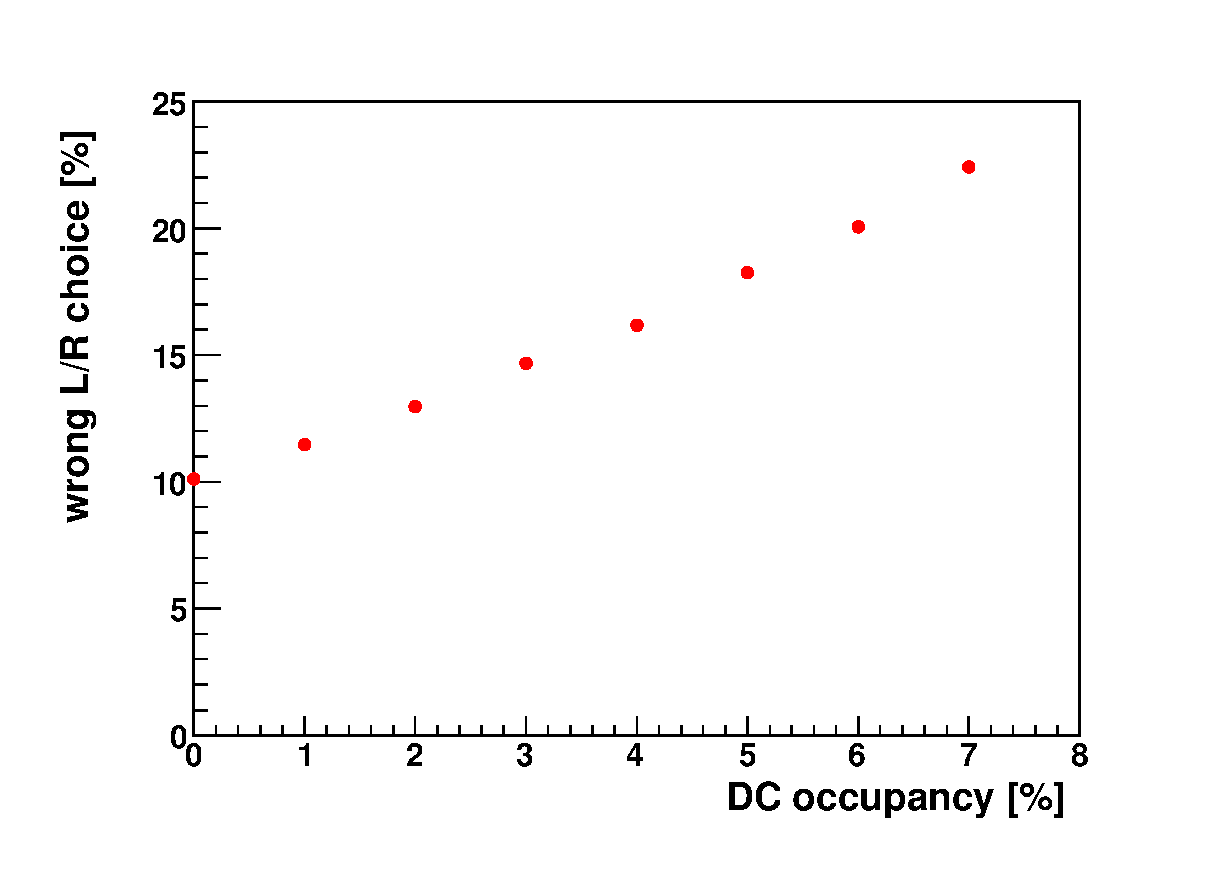
\includegraphics[width=0.7\textwidth]{wrongLR_vs_occupancy.eps}
\caption{\small{Probability to wrongly solve the left-right ambiguity as a function 
of the DC occupancy.}}
\label{sec_forward:pic_roadsincluster}
\end{figure}
%%%%%%%%%%%%%%%%%%%%%%%%%%%%%%%%%%%%%%%%%%%%%%%%%%%%%%%%%%%%%%%%%%%%%%%%%%%

\paragraph{Track Fitting:}

The final sets of hits are then sent to the Kalman Filter algorithm, as for the 
central part.  Because of the geometry of the Forward Tracker (measurements at 
approximately constant $z$), the state vector chosen is now:

\begin{equation}
\vec{x} = (x, y, u_x, u_y, Q/p)^T,
\end{equation}

\noindent
where $x$ and $y$ are the coordinates in a plane perpendicular to the beam axis, 
$u_x$ and $u_y$ are the slopes of the projected track in the $xz$ and $yz$ planes, 
respectively, and $Q/p$ is the charge divided by the momentum.

The first four components of this state vector are easily initialized at the last 
plane of Region~3.  The last component is estimated using the angles before (using a 
linear fit in Region~1) and after (using Region~3) the toroidal field, $\theta_1$ 
and $\theta_3$.  We then use the well known formula:

\begin{equation}
Q/p = \frac{\theta_3-\theta_1}{0.3\times \int{Bdl}},
\end{equation}

\noindent
with a parameterization of the field integral $\int{Bdl}$ as a function of the 
position in Region~1 (this parameterization is different for positively and negatively
charged particles).

The initial uncertainties on these components (used in the covariance matrix) were 
chosen to be 3~cm for the position terms, 80~mrad for the slopes, and 50\% for $Q/p$.

As for the central part, the fit is then stopped at the closest distance to the beam 
axis.  However, for some specific reactions, we may want to determine the vertex 
position more accurately, and the DC are then used in combination with the FST.  The 
key issue is then the accuracy of the extrapolation of the track parameters between 
the first DC plane and the last FST layer (located more than 2~m upstream).

\subsubsection{Matching with the FST}

The track finding procedure in the FST is quite simple, as the double layers are very 
close to each other, so track candidates are almost straight lines.  We therefore 
select combinations of strips producing three almost aligned points in space, 
pointing not too far from the beam axis.  The corresponding cuts have been optimized 
to identify at least 99\% of the \emph{reconstructable} tracks.

As the FST is always used with the DC, and not as a standalone tracker, we do not 
need \emph{a priori} to require a hit in each layer.  However, all the dead zones are 
aligned in the current design, so that a particle missing one layer will miss at least 
another one with a probability of around 99.5\%.  Besides, requiring only two out of 
three double layers increases the reconstruction of fake tracks by a large factor. 
We thus require three out of three double layers to define a track candidate in the 
FST.  The resulting acceptance efficiency is shown in Fig.~\ref{sec_forward:pic_FSTeff} 
as a function of the polar and azimuthal angles of the particles.

%%%%%%%%%%%%%%%%%%%%%%%%%%%%%%%%%%%%%%%%%%%%%%%%%%%%%%%%%%%%%%%%%%%%%%%%%%%
\begin{figure}[ht!]
\centering
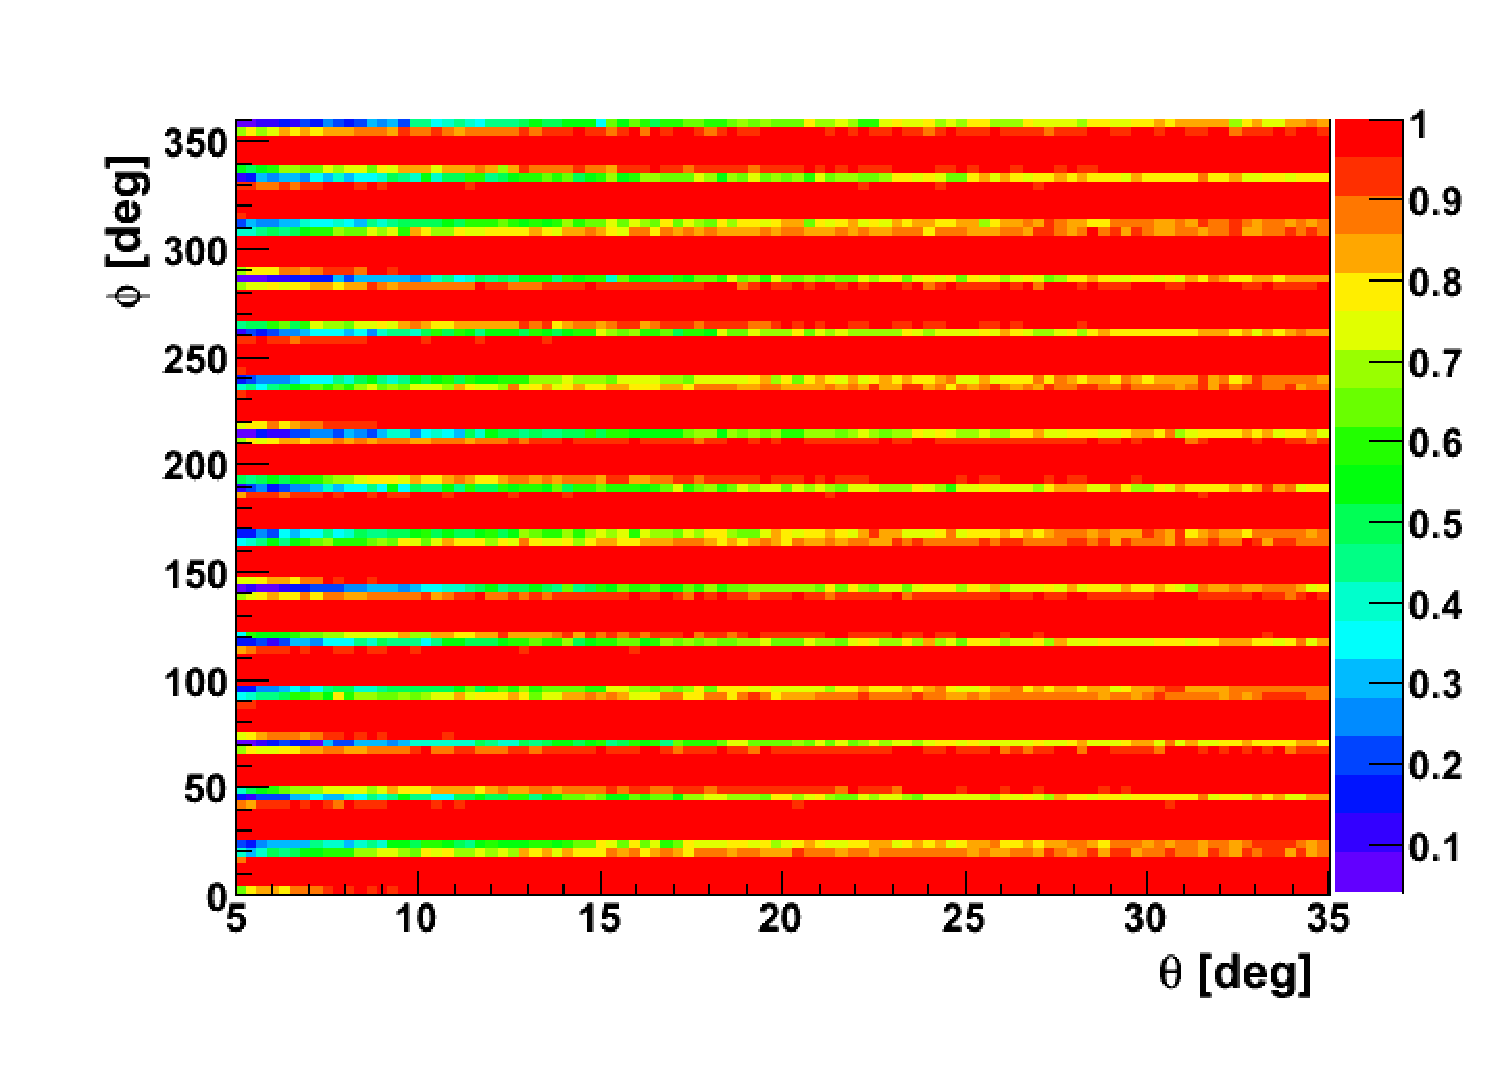
\includegraphics[width=0.7\textwidth]{FVT_2deff_phitheta_thintarget.eps}
\caption{\small{Acceptance efficiency of the FST as a function of the polar and 
azimuthal angles of the tracks, requiring three out of three double layers.}}
\label{sec_forward:pic_FSTeff}
\end{figure}
%%%%%%%%%%%%%%%%%%%%%%%%%%%%%%%%%%%%%%%%%%%%%%%%%%%%%%%%%%%%%%%%%%%%%%%%%%%

For a 1-mm long target, the integrated efficiency of the FST is:

\begin{equation}
\langle \epsilon \rangle = 92\%.
\end{equation}

\noindent
The next step is to be able to match track candidates from the FST and from the DC. 
To do this, we run the Kalman Filter algorithm on DC candidates, extrapolate down 
to the FST, and look for a \emph{close} FST candidate.  The accuracy of this 
extrapolation should be good enough not to match with another track (fake or not). 
Fig.~\ref{sec_forward:pic_matching} shows that, for a large fraction of tracks, the 
extrapolated position is within a few mm circle around the original position of the 
particle.  A 1-cm cut is therefore applied on the distance between the extrapolation 
and the FST track to match the two candidates.  This allows a 98\% matching efficiency 
without background; the effect of the DC occupancy (that deteriorates the accuracy of 
the fit) is shown in Fig.~\ref{sec_forward:pic_matcheff}.

%%%%%%%%%%%%%%%%%%%%%%%%%%%%%%%%%%%%%%%%%%%%%%%%%%%%%%%%%%%%%%%%%%%%%%%%%%%
\begin{figure}[ht!]
\centering
\includegraphics[width=0.49\textwidth]{CircleConfusion_theta15_proton_DCocc0_FVT0MHz.eps}
\includegraphics[width=0.49\textwidth]{CircleConfusion_theta15_proton_DCocc4_FVT40MHz.eps}
\caption{\small{$xy$ distribution of the DC track extrapolated down to the last FST 
layer with respect to the original position of the track. (Left): without any 
background; (right): with a 4\% occupancy in the DC.}}
\label{sec_forward:pic_matching}
\end{figure}
%%%%%%%%%%%%%%%%%%%%%%%%%%%%%%%%%%%%%%%%%%%%%%%%%%%%%%%%%%%%%%%%%%%%%%%%%%%

%%%%%%%%%%%%%%%%%%%%%%%%%%%%%%%%%%%%%%%%%%%%%%%%%%%%%%%%%%%%%%%%%%%%%%%%%%%
\begin{figure}[ht!]
\centering
\includegraphics[width=0.6\textwidth]{matchingEff_vs_occupancy.eps}
\caption{\small{FST-DC matching efficiency as a function of the DC occupancy.  A
4\% occupancy degrades the efficiency by around 10\%.}}
\label{sec_forward:pic_matcheff}
\end{figure}
%%%%%%%%%%%%%%%%%%%%%%%%%%%%%%%%%%%%%%%%%%%%%%%%%%%%%%%%%%%%%%%%%%%%%%%%%%%

When the matching is successful, it appears that the fit is too unstable to be 
performed in a single step.  We thus introduced some iterations as follows: in a 
first step, the Kalman Filter fits the track backwards, assuming a larger space 
resolution for the FST (7 times larger); the track is then extrapolated forwards, 
and refit using only the DC.  The final fit is performed backwards again, using the 
real resolution for the FST.  We are now able to derive the resolutions obtained in 
the Forward Tracker, and to study the effect of the FST.

\subsubsection{Tracking Performance}

The resolutions of momentum, polar angle $\theta$, azimuthal angle $\phi$, vertex 
position $z$, and distance of closest approach to the beam axis $b$ are presented in 
Fig.~\ref{sec_forward:pic_resolproton} for proton tracks at 15$^\circ$, using the DC 
alone, or in combination with the FST.  Fig.~\ref{sec_forward:pic_resolelectron} shows 
the same resolutions for electron tracks.  The effect of the DC occupancy on the 
resolution is very limited, as illustrated in Fig.~\ref{sec_forward:pic_phiresol} for 
the $\phi$ resolution.

%%%%%%%%%%%%%%%%%%%%%%%%%%%%%%%%%%%%%%%%%%%%%%%%%%%%%%%%%%%%%%%%%%%%%%%%%%%
\begin{figure}[ht!]
\centering
\includegraphics[width=0.29\textwidth]{DC_vs_DCFVT_theta15_sigmapop_DCocc4_FVT40MHz.eps}
\includegraphics[width=0.29\textwidth]{DC_vs_DCFVT_theta15_sigmatheta_DCocc4_FVT40MHz.eps}
\includegraphics[width=0.29\textwidth]{DC_vs_DCFVT_theta15_sigmaphi_DCocc4_FVT40MHz.eps}
\includegraphics[width=0.29\textwidth]{DC_vs_DCFVT_theta15_sigmaz_DCocc4_FVT40MHz.eps}
\includegraphics[width=0.29\textwidth]{DC_vs_DCFVT_theta15_sigmab_DCocc4_FVT40MHz.eps}
\caption{\small{Resolutions in $p$, $\theta$, $\phi$, $z$, and $b$ (distance of 
closest approach to the beam axis) for 15$^\circ$ protons with and without the FST. 
A 4\% occupancy in the DC and 40~MHz in the FST have been assumed.}}
\label{sec_forward:pic_resolproton}
\end{figure}
%%%%%%%%%%%%%%%%%%%%%%%%%%%%%%%%%%%%%%%%%%%%%%%%%%%%%%%%%%%%%%%%%%%%%%%%%%%

%%%%%%%%%%%%%%%%%%%%%%%%%%%%%%%%%%%%%%%%%%%%%%%%%%%%%%%%%%%%%%%%%%%%%%%%%%%
\begin{figure}[ht!]
\centering
\includegraphics[width=0.29\textwidth]{DC_vs_DCFVT_electrons_theta15_sigmapop_DCocc4_FVT40MHz.eps}
\includegraphics[width=0.29\textwidth]{DC_vs_DCFVT_electrons_theta15_sigmatheta_DCocc4_FVT40MHz.eps}
\includegraphics[width=0.29\textwidth]{DC_vs_DCFVT_electrons_theta15_sigmaphi_DCocc4_FVT40MHz.eps}
\includegraphics[width=0.29\textwidth]{DC_vs_DCFVT_electrons_theta15_sigmaz_DCocc4_FVT40MHz.eps}
\includegraphics[width=0.29\textwidth]{DC_vs_DCFVT_electrons_theta15_sigmab_DCocc4_FVT40MHz.eps}
\caption{\small{Resolutions in $p$, $\theta$, $\phi$, $z$, and $b$ (distance of 
closest approach to the beam axis) for 15$^\circ$ electrons with and without the 
FST.  A 4\% occupancy in the DC and 40~MHz in the FST have been assumed.}}
\label{sec_forward:pic_resolelectron}
\end{figure}
%%%%%%%%%%%%%%%%%%%%%%%%%%%%%%%%%%%%%%%%%%%%%%%%%%%%%%%%%%%%%%%%%%%%%%%%%%%

%%%%%%%%%%%%%%%%%%%%%%%%%%%%%%%%%%%%%%%%%%%%%%%%%%%%%%%%%%%%%%%%%%%%%%%%%%%
\begin{figure}[ht!]
\centering
\includegraphics[width=0.7\textwidth]{phiResol_vs_occupancy.eps}
\caption{\small{Evolution with the DC occupancy of the $\phi$ resolution (the 
$p$ independent term) in the forward tracker.}}
\label{sec_forward:pic_phiresol}
\end{figure}
%%%%%%%%%%%%%%%%%%%%%%%%%%%%%%%%%%%%%%%%%%%%%%%%%%%%%%%%%%%%%%%%%%%%%%%%%%%

If we compare with the original requirements from Table~\ref{intro_requirements}, 
we see that the DC design satisfies all of the proposed performances.  Concerning 
the FST, it largely improves the vertex determination (up to a factor 10 on $b$), 
and also allows a better determination of $p$ and $\phi$ at large momenta.

\subsubsection{Misalignments}

As for the BST, we implemented in Socrat the possibility to misalign the detectors 
or the magnetic fields.  For a given region of the DC, the following parameters can 
be misaligned:

\begin{itemize}
\item the distance $R$ to the target;
\item the tilt around its local $x'$ axis (25$^\circ$ being the nominal value);
\item the distance of the first wire to the beam axis.
\end{itemize}

\noindent
Two parameters of an FST double layer can also be misaligned.  These are:

\begin{itemize}
\item its azimuthal position $\phi$;
\item its position along the beam axis $z$.
\end{itemize}

\noindent
Finally, Socrat can misalign the toroidal field in $x$, $y$, and $z$, with respect 
to the rest of the spectrometer.

Due to the large number of parameters, we illustrate only the effect of misalignment 
in $R$ for Region~3 of the DC, and in $z$ for the torus, as shown in 
Fig.~\ref{sec_forward:pic_FTmisalign}.  We see that both the DC and the torus should 
be aligned within a fraction of a millimeter.  In general, our studies are consistent 
with the rule saying that a detector needs to be aligned within a fraction of its 
space resolution for a given parameter: e.g. less than 50~$\mu$m for the transverse 
position of the FST, and a few hundred microns for the longitudinal one (because of 
the angle of the tracks).

%%%%%%%%%%%%%%%%%%%%%%%%%%%%%%%%%%%%%%%%%%%%%%%%%%%%%%%%%%%%%%%%%%%%%%%%%%%
\begin{figure}[ht!]
\centering
\includegraphics[width=0.49\textwidth]{DCFVT_aligned_VS_DC3DR1mm_Deltapop.eps}
\includegraphics[width=0.49\textwidth]{DCFVT_aligned_VStorusDz10mm_Deltapop.eps}
\caption{\small{Effect of misalignments on the reconstructed momentum as a function 
of $p$: (left): $R$ translation of DC Region~3 by 1~mm; (right): $z$ translation of 
the toroidal field by 10~mm.}}
\label{sec_forward:pic_FTmisalign}
\end{figure}
%%%%%%%%%%%%%%%%%%%%%%%%%%%%%%%%%%%%%%%%%%%%%%%%%%%%%%%%%%%%%%%%%%%%%%%%%%%

\subsection{Conclusion}

We described in this section the program we developed for charged particle 
reconstruction with the {\tt CLAS12} spectrometer.  In the central and forward 
parts, track finding procedures, as well as a Kalman Filter algorithm, were 
successfully applied.  They provide for efficient reconstruction with resolutions 
that are in agreement with initial estimations and fulfill the physics requirements. 
The effect of the background has been quantified, and seems to be limited . 
Misalignments of all the detectors have also been studied, providing constraints on 
the position accuracy that will be needed, in particular for the BST.  For the 
Forward Tracker, we showed that a highly efficient matching can be obtained between 
the FST and DC tracks, and we quantify the large improvement of the FST on the 
vertex determination.

The global track reconstruction is however not yet finished.  More studies will be 
needed using GEANT4 simulations, particularly to study the effect of the correlated 
background on the tracking efficiency in the DC.  A vertex fit, gathering 
information from the central and forward regions, has to be developed.  Some smaller 
improvements can also be implemented, for example to take into account double hits 
from a single track in the DC.

\section{Expected Physics Performance}

We have used a series of programs to calculate the acceptance and 
reconstructed physics parameters for event types of interest.  The program 
CLASEV~\cite{clasev} served as an event generator and analysis program. 
Depending on the value of input flags, it generates certain types of events, 
that is, it produces a set of 4-momenta for the primary hadrons in the 
hadronic center-of-mass and allows some of them to decay into the final-state 
hadrons and transforms their momenta to the lab system.  For each final-state 
track, it calls FASTMC (our fast, parametric Monte Carlo program for
{\tt CLAS12}) to determine if the track falls within a fiducial acceptance 
window and to determine its final, smeared lab momentum.  It then produces 
selected physics analysis variables (e.g. missing mass) from calculations 
involving the smeared momenta of the tracks that were accepted. 
Fig.~\ref{massplot} shows the expected missing mass resolution expected for 
{\tt CLAS12} from FASTMC simulation studies based on the current design 
specifications for a number of different reactions.  For all cases studied, 
the results are quite encouraging in terms of identifying the missing 
particle cleanly for each reaction.  Our GEANT3 results are in accord
with the FASTMC results.

We also show some results from our FASTMC simulation of $e \pi^+$ events
in which the recoil baryon is detected by missing mass.  
Fig.~\ref{centralmassplot} shows the missing mass spectrum expected when
the $\pi^+$ is detected in the forward tracker (left) or central tracker
(right).  We have sufficient resolution to study resonant production and
to compare, for example, u-channel, s-channel and t-channel processes.

%%%%%%%%%%%%%%%%%%%%%%%%%%%%%%%%%%%%%%%%%%%%%%%%%%%%%%%%%%%%%%%%%%%%%%%%%%%
\begin{figure}[htbp]
\vspace{14.0cm}
\special{psfile=mm1.ps hscale=39 vscale=36 hoffset=0 voffset=160}
\special{psfile=mm2.ps hscale=39 vscale=36 hoffset=235 voffset=160}
\special{psfile=mm3.ps hscale=40 vscale=37 hoffset=0 voffset=-55}
\special{psfile=mm4.ps hscale=40 vscale=37 hoffset=240 voffset=-55}
\caption{\small{Simulation results from FASTMC highlighting the expected 
missing mass resolution of {\tt CLAS12} with the nominal design 
specifications for the tracking detectors (drift chambers and SVT).  Shown 
are the spectra for the reactions $ep \to e'\pi+X$ (UL), $ep \to e'K^+X$ (UR),
$ep \to e'p\pi^+X$ (LL), and $ep \to e\rho^+X$ (LR).}}
\label{massplot}
\end{figure}
%%%%%%%%%%%%%%%%%%%%%%%%%%%%%%%%%%%%%%%%%%%%%%%%%%%%%%%%%%%%%%%%%%%%%%%%%%%

%%%%%%%%%%%%%%%%%%%%%%%%%%%%%%%%%%%%%%%%%%%%%%%%%%%%%%%%%%%%%%%%%%%%%%%%%%%
\begin{figure}[htbp]
\vspace{6.0cm}
\special{psfile=clas12pipforward.eps hscale=39 vscale=36 hoffset=0 voffset=0}
\special{psfile=clas12pipcentral.eps hscale=39 vscale=36 hoffset=235 voffset=0}
\caption{\small{Simulation results from FASTMC highlighting the expected 
missing mass resolution of {\tt CLAS12} for events in which we detect only
a $\pi^+$ and the electron for two cases: on the left when the $\pi^+$
is detected in the forward tracker, and on the right when detected in
the central tracker.}}
\label{centralmassplot}
\end{figure}
%%%%%%%%%%%%%%%%%%%%%%%%%%%%%%%%%%%%%%%%%%%%%%%%%%%%%%%%%%%%%%%%%%%%%%%%%%%

\section{Safety and Quality Assurance Issues}

\subsection{Safety}

There are safety issues in the construction, installation, and operation
phases of the {\tt CLAS12} drift chamber and SVT projects that we address 
in this section.  Safety will be addressed from the start as an integral 
part of all activities and plans.  All of our workers will receive 
appropriate training prior to being permitted to perform any activities 
on the detectors.

\subsubsection{Drift Chamber}

Table~\ref{dc-safety} briefly summarizes the issues and the mitigation 
strategies employed for the drift chamber system.

%%%%%%%%%%%%%%%%%%%%%%%%%%%%%%%%%%%%%%%%%%%%%%%%%%%%%%%%%%%%%%%%%%%%%%%%%
\begin{table}[htbp]
\begin{center}
\begin{small}
\begin{tabular} {||c|c|c||} \hline \hline
{\bf Operation} & {\bf Issue}     &  {\bf Mitigation} \\ \hline
Cleaning parts  & Solvents & Use of non-volatiles; masks \\ \hline
Box assembly & Material handling, welding & Standard procedures \\ \hline
Stringing & Material handling  & Design overview, reviewed procedures \\ \hline
Installation & Material handling & Design overview, reviewed procedures \\ \hline
Gas delivery      & Flammability; ODH & Non-flammable mixture, small lines \\ \hline
Gas delivery      & Over/under pressure & Active controls, passive bubblers \\ \hline
LV power          & Over-heating & Each line individually fused \\ \hline
HV power          & Shock & Current-limited supplies, reviewed procedures \\ \hline
Routine operation & Sparking & Fast-trip supplies \\ \hline
Repair & Material handling & Design overview, reviewed procedures \\ \hline \hline
\end{tabular}
\end{small}
\caption{\small{Safety issues in the {\tt CLAS12} drift chamber project.}}
\label{dc-safety}
\end{center}
\end{table}
%%%%%%%%%%%%%%%%%%%%%%%%%%%%%%%%%%%%%%%%%%%%%%%%%%%%%%%%%%%%%%%%%%%%%%%%%

The only significant safety issues are in the construction, installation, 
and operation of the chambers.  During the construction phase, we receive 
a number of machined parts from industry that must be cleaned thoroughly 
before assembly into a chamber.  Our anticipated cleaning strategy is to 
use safe, non-volatile cleaning agents that are friendly to the environment 
and to human health.  All of our activities are coordinated by written 
procedures that are reviewed by our safety staff at the lab.

During construction of the chamber boxes, we handle heavy metallic items and 
bolt or weld certain items.  All of these activities are handled by personnel 
with adequate safety training, wearing suitable protective gear.  The designs 
of all mechanical assemblies are reviewed by trained mechanical engineers and 
experienced technicians.

During stringing of the chamber, the technicians and stringers work on 
elevated platforms.  The platform designs are reviewed in a similar fashion 
to the chamber mechanical designs, and all work is closely supervised by 
experienced technicians.

Operation of the chambers involves the use of a gas-handling system.  We use 
non-flammable gas mixtures delivered to the chambers at low pressure.  There 
are intermediate storage tanks filled with gas at moderate (a few atmospheres)
of pressure.  The gas-mixing and delivery system will be the same as the 
present {\tt CLAS} system with minor modifications, so we will continue to 
follow our present safety procedures that include some engineering controls 
in the gas-mixing shed to mitigate possible ODH conditions and extensive 
active and passive controls to mitigate over- and under-pressure conditions 
that could harm the drift chambers.

The normal operation also involves delivery of low-voltage power to the 
on-chamber amplifiers.  Although the low voltage (less than 8~V) means that 
there is no electrocution hazard, there is a potential for over-heating and 
fire ignition because of the relatively high currents involved.  Each supply 
is capable of supplying up to 50~mA of current.  Our mitigation strategy is 
to not allow more than 3~A of current on any output line, enforced by the 
placement of individual fuses on every wire that leaves the supply. 

The Hall B Drift Chamber Low Voltage (DCLV) supply and distribution system 
consists of 18 HP 6651A power supplies. Each power supply has a maximum 
current output of 8~VDC and 50~A of current. The power supplies are connected 
to the Hall B 120~VAC clean power located in the individual racks of the 
space frame that are protected by an electrical breaker panel. The supplies 
have a 10~A current limiting fuse for its own A.C. line protection.  The 
DCLV system supplies DC power to the drift chamber Signal Translator Boards 
(STBs). The output voltage can be set at the supply, as well as a current 
limit. In Hall B the current limits are individually set for each 
region/sector. The power is then supplied to the STBs via a distribution 
chassis.  Each chassis is safety interlocked and contains 3 bus bars 
(positive, negative, and earth ground), of which the positive and negative 
are connected to the individual STBs through current limiting fuses.  The 
individual fuses provide the nominal current draw plus 20\% for transient 
spikes. The distribution system for Region~3 was upgraded in 2003 to provide 
segmentation of the axial and stereo boards, thus reducing the damage of a 
permanent short by half. The upgrade consisted of adding new power wires 
from the distribution to the STBs and adding an additional breakout chassis. 
The breakout chassis provided individual fuses for each side of the STB in 
front of the distribution fuse.  Each breakout fuse is rated for the nominal 
current draw of its respective channel on the STB plus 40\% for transient 
spikes.  In the event of a short on the chamber there is a written procedure 
for changing out fuses located in the Hall B counting house and the drift 
chamber expert manual.  Monitoring of the supplies is done using a PC-based 
LabView program from the Hall B counting house.

Operation also involves the delivery of high-voltage to the drift chamber 
wires.  The operating voltages are between 1000 and 2000~V, depending on 
the section in question.  In all cases, the high voltage supplies are 
current-limited.  No channel can deliver more than 40~$\mu$A of current.  
Administrative procedures are in place to prevent accidental shocks from 
taking place.

The Hall B Drift Chamber High Voltage (DCHV) system consists of 3 CAEN 527 
supplies, with each containing up to 10 A934 (P/N) modules, distribution 
chassis, and software-based monitoring and control system.  Each module has 
a safety interlock that controls the output of power. The entire system has 
programmable firmware to set the current limit, voltage, and ramp rate, as 
well as system monitoring. The crate is connected to the Hall B clean power 
system and the A.C. input power is fused at the chassis. The modules output 
high voltage to a distribution system that consists of a summation and 
distribution chassis for the areas of the drift chamber. The current is 
limited to 20~$\mu$A output from the modules.  Monitoring and control is 
done via the DCHV TCL/TK program.

\subsubsection{SVT}

The only significant safety issues are in the construction, installation, 
and operation of the SVT.  During the construction phase, we receive 
a number of machined parts from industry that must be cleaned thoroughly 
before assembly.  Our anticipated cleaning strategy is to use safe, 
non-volatile cleaning agents that are friendly to the environment and to 
human health.  All of our activities are coordinated by written 
procedures that are reviewed by our safety staff at the lab.

The normal operation also involves delivery of low-voltage power to the 
on-board amplifiers.  Although the low voltage (less than 8~V) means that 
there is no electrocution hazard, there is a potential for over-heating and 
fire ignition because of the currents involved.  The design of the
low voltage system will include appropriate current fusing to ensure
safety to personnel and to the equipment.

Operation of the SVT also involves the delivery of high-voltage to the 
detector.  The design of the high voltage supplies will include 
over-current and over-voltage protection.   Administrative procedures are 
in place to prevent accidental shocks from taking place.

\subsection{Quality Assurance}

Quality Assurance (QA) begins before the procurement of components and 
detector construction and continues beyond detector installation and 
commissioning.  This section details plans for QA for the drift chambers
and SVT for {\tt CLAS12}.

\subsubsection{Drift Chambers}

QA issues include not only the drift chambers themselves, but also the
associated high voltage system, low voltage system, gas system, and the 
actual environment the detector lives in.  There will be six identical 
units of each of three detector regions, for a total of 18 drift chambers. 
The challenge here will be to tightly control detector fabrication, 
stringing, instrumentation, and testing, while staying within the project's 
budget and schedule.  The following summary outlines some of the QA 
procedures that we will be implementing.

The electronics components will be accepted from the vendor by the JLAB Fast 
Electronics Group (FEG).  The FEG will inspect, test, and clean all 
components in accordance with written procedures that they will develop.  
All components will be sealed in anti-static bags and stored in a proper 
environment until needed.  Written certifications will be kept for all 
components.

The detector frame or box will be a mechanical assembly. This assembly will 
be built on an alignment fixture.  Precision positioning pins to locate 
reference points to the actual wire positions will be one of the features of 
the fixture. The JLAB survey group will be involved in this process from its 
inception.  Each completed assembly will be surveyed to verify it is within 
tolerance. The detector frame or box will then be cleaned before it enters the 
clean room for final component assembly and stringing.

All of the components will be inspected and cleaned prior to use as it is 
critical for maximizing detector lifetime.  Written procedures will be 
followed and records will be kept to identify the cleaning and inspection 
status of all components. Components will be stored in sealed bags in the 
clean room where feasible.

The {\tt CLAS12} drift chambers will be strung in a clean room environment. 
Technicians will wear clean room coats, gloves, shoe covers, and hair nets. 
Only clean gloves and clean tools will come into contact with the detector 
and its components.  All technicians who work in the clean room will be 
trained in proper clean room practices.  Written cleaning procedures and 
schedules will be developed to insure proper clean room maintenance. 
Supervisors will frequently inspect all areas to verify proper practices are 
followed.

Written procedures will be developed from the prototype experience for all 
detector assembly and stringing steps.  Fabricators and stringers will be 
trained by experienced persons in all required steps and procedures. They 
will be closely supervised to ensure compliance with written procedures and 
to prevent any deviation from accepted practice. 

At the end of each stringing shift, the wires will be tested for proper 
tension using a magnetic field and variable frequency oscillator. The 
frequency measured at the wires first fundamental for that length wire will 
be used to determine the wires tension. Wires with out of specification 
tension will be removed and new wires will be strung in their place. This test 
also verifies proper continuity of the wire from pin to pin. It will also 
identify crossed or twisted wires because those will show a decrease in 
signal amplitude.

The next tests are a redundant check for shorted or twisted wires missed 
during visual inspection and tension testing.  Prior to signal and high 
voltage board installation, the field and guard wire layers are wire wrapped. 
Once the high voltage side is wrapped, a multimeter will be used to determine 
if there are any shorts between layers or between and sense wires and the 
wire wrapped layers.  A multimeter will also be used to determine shorts and 
twisted wires in the same layer by measuring the resistance of each wire 
between the wire-wrap side and the pin on the opposite side. Since wire 
lengths are all known, the resistance of each wire is also known. Twisted 
wires will have much lower resistance than would be expected from that 
wire length.  The high voltage boards are installed and connections are made. 
A multimeter is then used to measure the resistance between sense layers. 
There should be infinite resistance between layers, and any other result 
indicates a short or twisted pair. The multimeter is then used to measure 
the resistance from the signal side of the wire to the high voltage bus. 
This should read $\approx$1~M$\Omega$, which is the value of the  
current-limiting resistor in the circuit.  A reading of 0.5~M$\Omega$ 
indicates a shorted or twisted pair.

Final testing includes high voltage tests and cosmic ray tests before and 
then after the final cabling and patch panel installation. The detector will 
then be stored in a temperature and humidity controlled area until 
installation. 

\subsubsection{SVT}

QA planning for the SVT system includes the following areas:

\begin{itemize}

\item Bench testing of each of the individual components of the SVT hardware
prior to module assembly.  This includes the silicon sensors, readout
chips, circuit boards, wire bonds, and cabling;

\item Testing of complete stave assemblies and modules prior to assembling
the detector as a unit;

\item Encapsulation of the wire bonds to prevent breakage or stress;

\item Including fiducial marks on all custom silicon components for alignment;

\item All assembly will be done in a clean room following established clean
room conventions;

\item Use of custom fixtures to prevent damage during shipment of components;

\item Use of alignment markers on the support structure for detector 
installation.
\end{itemize}

The quality assurance planning is being done in conjunction with a
value engineering (VE) approach for the design.  It is expected that the
VE for the SVT will improve the QA rating for the design.  The steps that
are being taken include:

\begin{itemize}

\item Use of one silicon sensor design for the barrel SVT and one design for 
the forward SVT for a total of only two total different sensors in the
system.  This allows for a lower number of spares to be purchased and
also allows for the possibility that sensor blocks can be interchanged
between regions;

\item The SVT design employs previously design readout chips.  The design
of these chips has therefore been extensively studied and detailed
performance evaluations have been completed;

\item Common circuit boards and electronic components will used for the
barrel and forward SVT.  These boards will follow industry and JLab
standards for design;

\item Whenever possible, the SVT design makes use of ``off-the-shelf''
components to improve reliability.
\end{itemize}

\subsection{Conformance with JLab ES\&H Manual}
	
All activities will be analyzed in accordance with the JLAB ES\&H Manual 
to identify any and all hazards associated with the work and any and all 
safety requirements mandated.  All persons involved and all persons in the 
vicinity will be briefed on all potential hazards involved in all activities.
However, all activities are considered low risk, common, and routine in 
nature and are all fully covered by the ES\&H Manual.

Many operations will be performed around and in the vicinity of equipment 
and other activities.  Procedures to identify and mitigate risks due to
trip and fall hazards will be developed.  Similar procedures will be
developed for work involving the use ladders, work platforms, and scaffolds. 
Standard safety procedures will be followed for all work involving the use
of cranes and hoists.  Instrumenting, testing, and troubleshooting the 
detectors may require Class 1 Mode 1 and Class 1 Mode 2 limited testing and 
diagnostics and will be performed according to EH\&S requirements.








